\documentclass[twoside]{projektInzynierskiMS}
\usepackage{polski}
\usepackage[utf8]{inputenc}
\usepackage{amsmath}
\usepackage{graphicx}
\usepackage{hyperref}
%\drukJednostronny

%% tytuł promotor iautor (\title to komenda standardowa)
\title{System obsługi Biblioteki Wydziału Matematyki Stosowanej}
\promotor{dr inż. Zdzisław Sroczyński}


%% każdy autor musi mieć 4 argumenty: imię nazwisko, nr albumu, procent wkładu, opis wkładu
\autor{Karolina Chrząszcz}{252525}{1} {Projekt interfejsu aplikacji mobilnej, implementacja aplikacji na system Android}
	
\autor{Szymon Górnioczek}{252252}{1} {Wykonanie aplikacji serwerowej i panelu administracyjnego dla bibliotekarza}

\autor{Tomasz Kryg}{225183}{98}	{Projekt interfejsu aplikacji mobilnej, implementacja aplikacji na system iOS}
	
	


%% dedykacja mile widziana
\dedykacja{Karolinie\\Szymonowi\\Tomkowi}
%\NumeryNaPoczatku
%% numeracja wzorów tu włączona typu (1.2.3), ta druga to typu (1.2), domyślnie typu (1)
%\subsectionWzory
% \sectionWzory  

%\rozdzialy


%\literowaNumeracjaDodatkow %% włączy numerację dodatków literami
%\rzymskaNumeracjaDodatkow  %%włączy numerację dodatków liczbami rzymskimi

%% wyłączenie wyjaśnień:
\bezWyjasnien

%% standardowe komendy \newtheorem  działają jak woryginale
\newtheorem{tw}{Twierdzenie}%[subsection]
\newtheorem{twa}{Twierdzenie}%[section]
\newtheorem{dd}{Definicja}%[subsection]

\begin{document}

Książka -- jeden z najbardziej podstawowych przedmiotów. Każdy z nas, nawet jeśli nie lubi czytać, niejednokrotnie w swoim życiu z jakiejś korzystał. Może służyć rozrywce, ale przede wszystkim szeroko pojętej edukacji. Każda przeczytana książka pomaga rozwinąć myślenie jak i kreatywność czytelnika. Każde przeczytane zdanie rozwija zdolność wypowiadania się. 
Każde przeczytane słowo pozwala poszerzyć zdolności językowe.

W dzisiejszych czasach, książki są coraz częściej pomijane kosztem innych rozrywek, takich jak gry komputerowe, kino czy telewizja, które z roku na rok wypychają książkę na dalszy plan. Jak wynika z raportu Biblioteki Narodowej \cite{raportBN}, w roku $2016$ jedynie $37\%$ Polaków przeczytało choć jedną książkę. Mogłoby się więc wydawać, że wchodzenie na rynek książek nie jest najlepszym pomysłem. Jednak istnieją książki, które posiadają często wiadomości niezmienne i nie służą rozrywce, a przede wszystkim pozyskiwaniu wiedzy. Są to między innymi książki z działów ścisłych dotyczących bezpośrednio matematyki. Przykładowo ciąg Fibonacciego omówiony w~roku $1202$ przez Leonarda z Pizy, do dziś został opisany i wykorzystany w wielu książkach związanych z~różnorodnymi dziedzinami. Z przytoczonego przykładu wynika, że książki dotyczące matematyki czy też fizyki, bardzo często zawierają dużo wiedzy, nawet w czasach współczesnych. Wszystko ewoluuje, jednak prawa natury pozostają niezmienne.

Współcześnie doszliśmy do punktu, w którym książka zaczyna mieć znaczenie przede wszystkim edukacyjne. Na uczelniach całego świata, książki są synonimem wiedzy, ponieważ bardzo często profesorzy i doktorzy kształcili się za pomocą takich samych materiałów co ich dzisiejsi uczniowie. Z tego powodu biblioteki -- szczególnie na początku semestru -- muszą zmagać się z dużymi ilościami studentów, chcącymi poszukać potrzebnych im książek oraz sprawdzić ich ilość i dostępność, aby później je wypożyczyć. Jest to problem zarówno dla pracowników biblioteki jak i dla studentów. Bibliotekarze są zajęci sprawdzaniem tych samych informacji dla każdego studenta z osobna. Natomiast uczniowie są zdenerwowani sporymi kolejkami i tłumem ludzi, który zniechęca do odwiedzania bibliotek.

\section{System obsługi biblioteki}

Korzystając z książek naukowych i z własnego doświadczenia, postanowiliśmy stworzyć system dla Biblioteki Wydziału Matematyki Stosowanej Politechniki Śląskiej w Gliwicach. Głównym celem systemu jest posiadanie informacji o zbiorach biblioteki wydziałowej i łatwe udostępnianie ich studentom. Podstawą jest prosty interfejs dla administratora uzupełniającego pozycje książek w systemie, jak i dla studenta chcącego szybko sprawdzić dostępność wybranej książki w bibliotece o~dowolnej porze, bez potrzeby wychodzenia z domu.

\begin{figure}[h]
  \centering
  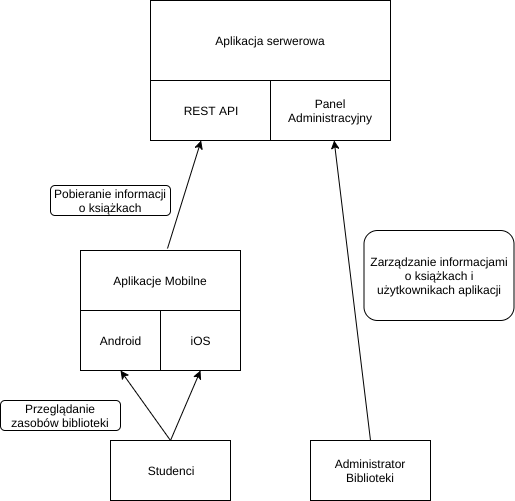
\includegraphics[width=0.8\linewidth]{img/bibsys/SystemDiagram.png}
  \caption{System obsługi biblioteki}
  \label{fig:adminLogin}
\end{figure}

Jednym z typów aplikacji będzie aplikacja webowa. Powinna zapewnić administratorowi pracującemu w bibliotece prostą obsługę bazy danych. Szybkie katalogowanie dostępnych woluminów oraz aktualizowanie informacji na temat dostępności.

Drugim typem aplikacji obsługujących bibliotekę będą aplikacje na smartfony. Zostaną stworzone dwie aplikacje mobilne, każda na oddzielny system: Android oraz iOS w celu poszerzenia grupy odbiorców na wydziale. Pozwolą one na przeszukanie biblioteki pod względem dowolnej szukanej frazy oraz dostarczą informacji o~wszystkich książkach i ich dostępności w bibliotece.


\section{Aplikacja serwerowa}
Aplikacja serwerowa LibraryApp, stanowi backend systemu bibliotecznego oraz zapewnia narzędzia dla bibliotekarza i administratora systemu, pozwalające na zarządzanie aplikacją. Głównymi zadaniami tej aplikacji są:
\begin{itemize}
	\item zarządzanie użytkownikami i~ich uprawnienami,
	\item zarządzanie bazą danych,
	\item zarządzanie informacją na temat woluminów biblioteki wydziałowej poprzez panel administracyjny,
	\item integracja aplikacji mobilnych poprzez usługę, dającą dostęp do informacji znajdujących się w~bazie danych.
\end{itemize}

\subsection{Użyte frameworki}

Do stworzenia aplikacji został wykorzystany \textit{Django}. Framework ten dostarcza rozwiązania takie jak:
\begin{itemize}
	\item system autoryzacji użytkowników \cite{DjangoAuth},
	\item możliwość zdefiniowania modelu danych kodem pythonowym oraz ORM wysokiego poziomu \cite{DjangoORM},
	\item automatycznie generowany i kompletny panel administracyjny \cite{DjangoAdmin},
	\item narzędzie do tworzenia serwisów webowych - \textit{Django REST framework} \cite{DjangoRest},
	\item wsparcie dla wielojęzycznych aplikacji (w tym język polski) \cite{DjangoTranslation},
\end{itemize}
które kompletnie pokrywają potrzeby aplikacji LibraryApp. Oprócz tego, jak można przeczytać na oficjalnej stronie \textit{Django} \cite{DjangoOfficial}, framework jest zaprojektowany~w taki sposób, aby robić częste zadania web-deweloperskie szybko i prosto. W praktyce oznacza to, że powstaje mało kodu aplikacji, dzięki czemu będzie on łatwiejszy do zrozumienia i modyfikowania. Obszerna i aktualna dokumentacja, dostępna na stronie projektu oraz duża społeczność korzystająca z \textit{Django} sprawia, że rozwój aplikacji jest łatwiejszy.

\subsubsection{Modele Django}
W \textit{Django} modele danych definiuje się jako klasy Python, które dziedziczą po \verb`django.db.models.Model` \cite{DjangoModel}. Na podstawie takiej klasy \textit{Django} automatycznie generuje tabele w bazie danych, każdy atrybut modelu reprezentuje pole w tabeli. Przykładowo, z modelu zdefniowanego w ten sposób:

\begin{verbatim}
class Category(models.Model):
    category_id = models.CharField(
        max_length=200,
        unique=True,
        verbose_name='Id kategorii'
    )
    category_name = models.TextField(
        verbose_name='Nazwa kategorii'
    )
\end{verbatim}
zostanie wygenerowana tabela w bazie danych:
\begin{verbatim}
CREATE TABLE `libraryapp_category` (
	`id`	integer NOT NULL PRIMARY KEY AUTOINCREMENT,
	`category_id`	varchar(200) NOT NULL UNIQUE,
	`category_name`	text NOT NULL
);
\end{verbatim}

\subsection{Model danych}

Model danych został zaprojektowany na podstawie specyfikacji, którą określił pracownik odpowiedzialny za działanie biblioteki. Wszystkie definicje modeli znajdują się w pliku \verb`/libproject/libraryapp/models.py`.

\subsubsection{Model Book}

Model ten został zaprojektowany na podstawie zakładki \verb`KSIAZKA` w arkuszu \verb`dane-prog-bibl.xlsx`, wchodzącego w skład specyfikacji. Model \verb`Book` jest zdefiniowany jako model \textit{Django} i składa się z pól:

\begin{itemize}
	\item \verb`signature_ms`, \\
		typu: \verb`IntegerField`, \\
		odpowiada danym z kolumny: SYG\_MS,
	\item \verb`signature_bg`, \\
		typu: \verb`CharField`, \\
		odpowiada danym z kolumny: SYG\_BG,
	\item \verb`responsibility`, \\
		typu: \verb`TextField`, \\
		odpowiada danym z kolumny: OZN\_OPDOW,
	\item \verb`title`, \\
		typu: \verb`CharField`, \\
		odpowiada danym z kolumny: TYTUL,
	\item \verb`volume`, \\
		typu: \verb`CharField`, \\
		odpowiada danym z kolumny: TOM,
	\item \verb`year`,\\
		typu: \verb`IntegerField`, \\
		odpowiada danym z kolumny: ROK,
	\item \verb`isbn_issn`, \\
		typu: \verb`CharField`, \\
		odpowiada danym z kolumny: ISBN/ISSN,
	\item \verb`type`, \\
		typu: \verb`CharField`, \\
		odpowiada danym z kolumny: TYP, \\
		przyjmuje wartości: \verb`'podręcznik'`, \verb`'inny'`, \verb`'zbiór zadań'`,
	\item \verb`availability`, \\
		typu: \verb`CharField`, \\
		odpowiada danym z kolumny DOSTEPNOSC, \\
		przyjmuje wartości: \verb`'dostępna'`, \verb`'wypożyczona'`, \verb`'czytelnia'`.
	\item \verb`categories`, \\
		typu: \verb`ManyToManyField`, \\
		odpowiada danym z zakładki PRZYPISANIE\_KATEGORII.
\end{itemize}

\subsubsection{Model Category}

Model ten został zaprojektowany na podstawie zakładki \verb`KATEGORIE` w arkuszu \verb`dane-prog-bibl.xlsx`.
Model \verb`Category` jest zdefiniowany jako model \textit{Django}, składa się z pól:

\begin{itemize}
	\item \verb`category_id`, \\
		typu: \verb`CharField`, \\
		odpowiada danym z kolumny: ID\_KATEGORII,
	\item \verb`category_name`, \\
	typu: \verb`TextField`, \\
	odpowiada danym z kolumny: KATEGORIA.
\end{itemize}

\subsection{Główne klasy}

Oprócz modeli opracowanych na podstawie dostarczonych danych, zostały zaprojektowane jeszcze klasy takie jak: \verb`CategoryTree`, \verb`Dictionary`, \verb`query`.

\subsubsection{Klasa CategoryTree}

Ze względu na wymagania opisane w punktach \textit{10 Kategoria główna} i \textit{11 kategoria szczegółowa}, dokumentu \verb`BIBLIOTEKA-program.docx`, dotyczące podziału kategorii na ,,kategoria główna'' i ,,kategoria szczegółowa'', została zaimplementowana klasa, która przedstawia tę relację między kategoriami. Kategoria główna to taka, której id jest postaci \verb`G_x`, gdzie \verb`x` to ciąg cyfr, na przykład \textbf{G\_00:ALGEBRA}.
 Kategoria główna może mieć kategorie szczegółowe, których id jest postaci \verb`G_x-S_y`, gdzie \verb`x` i \verb`y` to ciągi cyfr, część znajdująca się przed \verb`-` to id kategorii głównej. Zatem kategoria \textbf{G\_00-S\_04:algebry Boole’a}, jest kategorią szczegółową kategorii \textbf{G\_00:ALGEBRA}. 
 
Klasa \verb`CategoryTree` składa się z pól:
\begin{itemize}
	\item \verb`main_category`, 
		zawiera obiekt \verb`Category`,
		odpowiadający kategorii głównej,
	\item \verb`subcategories`, 
		zawiera tablicę obiektów \verb`Category`,
		odpowiadającym kategoriom szczegółowym.
\end{itemize}
Przykład:
\begin{verbatim}
{
    "main_category": {
        "category_id": "G_22",
        "category_name": "TOPOLOGIA"
    },
    "subcategories": [{
            "category_id": "G_22-S_00",
            "category_name": "topologia ogólna"
        },
        {
            "category_id": "G_22-S_01",
            "category_name": "topologia algebraiczna"
        }
    ]
}
\end{verbatim}

\subsubsection{Klasa Dictionary}
W celu dostarczenia do aplikacji mobilnych informacji o wartościach jakie mogą przyjmować niektóre pola w bazie danych oraz ułatwić w przyszłości modyfikowanie zakresu tych wartości, została zaimplementowana klasa \verb`Dictionary`. Obiekt tej klasy składa się z pól:
\begin{itemize}
	\item \verb`types`, \\
	typ: tablica zawierająca wartości jakie może przyjąć pole \verb`Book.types`,
	\item \verb`availability_types`, \\
	typ: tablica zawierająca wartości jakie może przyjąć pole \verb`Book.availability`.
\end{itemize}


\begin{verbatim}
{
    "availability_types": [
        "dostępna",
        "wypożyczona",
        "czytelnia"
    ],
    "types": [
        "podręcznik",
        "inny",
        "zbiór zadań"
    ]
}
\end{verbatim}

\subsubsection{Klasa query}
Obiekt klasy \verb`query` definiuje kryteria, według których, serwis zwróci książki. Klasa \verb`query` składa się z pól:
\begin{itemize}
	\item \verb`filters` -- obiekt definiujący filtry pól książek. Pola obiektu \verb`filters` są opcjonalne. Aby otrzymać książki, których tytuł jest równy pewnej wartości, obiekt \verb`filters` należy zdefiniować w następujący sposób:
	
	\begin{verbatim}
	"filters":{
	    "title":"wartość"
	}
	\end{verbatim}
	
Aby otrzymać z serwisu książki, których tytuł zawiera jakiś literał, obiekt \verb`filters` należy zdefiniować w następujący sposób:
	\begin{verbatim}
	"filters":{
	    "title__contains":"wartość"
	}
	\end{verbatim}
	
Filtry pozostałych pól definiujemy analogicznie. Filtrowanie po wielu polach zdefiniowane jest w następujący sposób:

	\begin{verbatim}
	"filters":{
	    "title__contains":"wartość",
	    "responsibility__contains": "GŁ",
	    "year":2003
	}
	\end{verbatim}
	
\item \verb`categories` -- tablica id kategorii, zwrócone książki zawierają jedną z kategorii podanych w tablicy. Przykład:

	\begin{verbatim}
	"categories":["G_00","G_01-S23"]
	\end{verbatim}

Aby otrzymać z serwisu książki, które posiadają konkretny zestaw kategorii, należy zdefiniować obiekt \verb`filter`:
 
	\begin{verbatim}
	"filters":{
	    "categories":["G_00","G_01-S23"]
	}
	\end{verbatim}

\item \verb`pagination` -- klasa pozwalająca na zdefiniowanie otrzymanego wycinka danych, zapobiega to zwróceniu zbyt dużej liczby danych jednoczesnie. Obiekt zawieta pola 
\begin{itemize}
	\item \verb`offset` -- definiuje ile pierwszych pozycji odrzucić,\\
	typu: \verb`unsigned int`,
	\item \verb`limit` -- definiuje ile pozycji może zostać zwróconych maksymalnie, podczas jednego zapytania,\\
	typu: \verb`unsigned int`.
\end{itemize}
 

\end{itemize}

Przykładowy obiekt \verb`query`:

\begin{verbatim}
"query":{
    "filters": {
        "responsibility__contains": "GŁ",
        "availability":"dostępna"
    },
    "categories":["G_00"],
    "pagination": {
        "offset":20,
        "limit":10
    }
}
\end{verbatim}

\subsection{Usługi}
Aplikacja serwerowa zapewnia usługi dające dostęp do informacji zawartych w~bazie danych. Usługi dostępne są za pomocą REST Api na środowisku uczelnianym pod adresem \verb`157.158.16.217:8000`. Do korzystania z usług nie jest wymagana autoryzacja.

\subsubsection{Usługa dostarczająca książki}
Usługa ta zwraca listę książek (\verb`book`), według kryterium zdefiniowanego przez obiekt \verb`query`.

Zapytanie:
\begin{itemize}
	\item Enpoint: \verb`/books`,
	\item Method: \verb`POST`,
	\item Headers: \verb`"Content-Type":"application/json"`,
	\item Body: \verb`JSON (application/json): query`,
\end{itemize}

Odpowiedź:
\begin{itemize}
	\item Tablica obiektów \verb`Book`.
\end{itemize}

Przykład odpowiedzi:
\begin{verbatim}
[{
    "signature_ms": 601,
    "signature_bg": "",
    "responsibility": "JAGŁOM I.M.; BOŁTIANSKI W.G.",
    "title": "Figury wypukłe",
    "volume": "",
    "year": 1955,
    "isbn_issn": "",
    "type": "inny",
    "availability": "dostępna",
    "categories": [{
        "category_id": "G_05-S_03",
        "category_name": "geometryczne pojęcie wypukłości"
    }]
}]
\end{verbatim}

\subsubsection{Usługa dostarczająca kategorie}
Usługa ta zwraca listę wszystkich kategorii przedstawionych jako obiekt \verb`CategoryTree`. 

Zapytanie:
\begin{itemize}
	\item Enpoint: \verb`/categories`,
	\item Method: \verb`GET`,
	\item Headers: \verb`"Content-Type":"application/json"`,
\end{itemize}

Odpowiedź:
\begin{itemize}
	\item Tablica obiektów \verb`CategoryTree`.
\end{itemize}

Przykładowa odpowiedź:

\begin{verbatim}
[{
        "main_category": {
            "category_id": "G_00",
            "category_name": "ALGEBRA"
        },
        "subcategories": [{
            "category_id": "G_00-S_00",
            "category_name": "algebra matematyczna"
        }]
    },
    {
        "main_category": {
            "category_id": "G_01",
            "category_name": "ANALIZA"
        },
        "subcategories": [{
            "category_id": "G_01-S_00",
            "category_name": "analiza matematyczna"
        }]
    }
]
\end{verbatim}


\subsubsection{Usługa dostarczająca słownik}
Zwraca obiekt \verb`Dictionary` zawierający wszystkie typy książek oraz typy ich dostępności.

Zapytanie:
\begin{itemize}
	\item Enpoint: \verb`/dictionary`,
	\item Method: \verb`GET`,
	\item Headers: \verb`"Content-Type":"application/json"`,
\end{itemize}

Odpowiedź:
\begin{itemize}
	\item Obiekt \verb`Dictionary`.
\end{itemize}

Przykładowa odpowiedź:

\begin{verbatim}
{
    "types": [
        "podręcznik",
        "inny",
        "zbiór zadań"
    ],
    "availability_types": [
        "dostępna",
        "wypożyczona",
        "czytelnia"
    ]
}
\end{verbatim}

\subsection{Wdrażanie}
Aby uruchomić aplikację wymagany jest jedynie zainstalowany \textit{python3.6}. Aplikację można uruchomić w systemach Linux, OS X~i Windows \cite[s. 140]{djangobook}, ten rozdział jednak opisuje proces wdrażania w systemie Linux. Skrypty załączone razem z aplikacją (\verb`setup_app.sh` oraz \verb`boot_script.sh`), są skryptami bashowymi, działającymi pod systemem Linux. 

\subsubsection{Wirtualne środowisko}
Wszystkie zależności potrzebne do uruchomienia aplikacji są instalowane wewnątrz wirtualnego środowiska, dzięki czemu proces wdrażania można~w dużej części zautomatyzować. Aby móc stworzyć wirtualne środowisko należy zainstalować paczkę \textit{virtualenv} korzystająć z polecenia:
\begin{verbatim}
sudo pip3 install virtualenv
\end{verbatim}


\subsubsection{Pobranie aplikacji}

Aplikacja jest dostępna na repozytorium \href{https://github.com/szymongor/library}{github.com/szymongor/library}, aby ją pobrać można skorzystać~z \textit{git} lub pobrać paczkę~w formie \textit{zip}~i rozpakować na maszynie, zalecane jest jednak użycie \textit{gita}, ułatwi to~w przyszłości nanoszenie zmian~w aplikacji. Szczegóły dotyczące instalacji \textit{gita} dostępne są na stronie \href{https://git-scm.com/book/en/v2/Getting-Started-Installing-Git/}{git-scm.com/book/en/v2/Getting-Started-Installing-Git/}. 

Aby ściągnąć aplikację poprzez \textit{git} należy skorzystać~z komendy:

\begin{verbatim}
git clone https://github.com/szymongor/library.git
\end{verbatim}
w rezultacie, powinien się pojawić folder \verb`library` w obecnej lokalizacji. Należy otworzyć folder z aplikacją używająć komendy \verb`cd library`. Katalog powinien zawierać:

\begin{itemize}
	\item \verb`boot_script.sh` - skrypt bashowy, uruchamiający aplikację,
	\item \verb`librarysite` - folder zawierający pliki aplikacji \textit{Django},
	\item \verb`properties.py` - plik zawierający konfigurację aplikacji,
	\item \verb`setup_app.sh` - skrypt bashowy, automatycznie konfiguruje środowisko,
	\item \verb`libraryapp` - folder z plikami aplikacji Django,
	\item \verb`manage.py` - skrypt \textit{Django}, do zarządzania aplikacją,
	\item \verb`requirements.txt` - lista zależności potrzebna do uruchomienia aplikacji, zostanie automatycznie załadowana przez skrypt \verb`setup_app.sh`,
	\item \verb`static` - folder z plikami statycznimi aplikacji.
\end{itemize}



\subsubsection{Konfiguracja aplikacji}

Aby skonfigurować aplikację należy edytować plik \verb`properties.py`, np. używając polecenia:
\begin{verbatim}
nano properties.py
\end{verbatim}

Przykładowa konfiguracja aplikacji:
\begin{verbatim}
PROJECT_PATH="/home/biblio/libproject/"
VENV="libvenv"
HOST="157.158.16.217:8000"
LOG_FILE="logs"
SECRET_KEY='f1b($dr1^t$8!#$#!a^8xmj0+#$pnaramf1r^xd(t5a%ghjai_'
ALLOWED_HOSTS=['127.0.0.1','localhost','157.158.16.217']
USER_NAME="BibliotekaMS"
PASSWORD="tajne_haslo_nalezy_zmienic"
MAIL="admin@mail.com"
\end{verbatim}

Plik konfiguracyjny składa się z pól:
\begin{itemize}
	\item \verb`PROJECT_PATH` (!) -- lokalizacja folderu library z aplikacją,
	\item \verb`VENV` (*) -- nazwa wirtualnego środowiska, jeśli jeszcze nie zostało utworzone, skrypt \verb`setup_app.sh` automatycznie utworzy wirtualne środowisko o takiej nazwie,
	\item \verb`HOST` (!) -- adres IP oraz port na które zostanie wystawiona aplikacja,
	\item \verb`LOG_FILE` (*) -- nazwa pliku z logami aplikacji,
	\item \verb`SECRET_KEY` (!) -- tajny klucz, typu string, długości 50, używany przez \textit{Django} np. do podpisywania plików cookies i autoryzacji,
	\item \verb`ALLOWED_HOSTS` (!) -- tablica adresów hostów/domen, które mogą serwować aplikację, zabezpieczenie ze strony \textit{Django} przed atakami typu Host Header Injection,
	\item \verb`USER_NAME` (*) -- nazwa użytkownika panelu administracyjnego, mającego uprawnienia administratorskie~w aplikacji,
	\item \verb`PASSWORD` (!) -- hasło użytkownika,
	\item \verb`MAIL` (*) -- adres email użytkownika.
\end{itemize}

Pola oznaczone "!" należy edytować, pola oznaczone "*" można edytować lub pozostawić niezmienione.

\subsubsection{Uruchomienie aplikacji}
Podczas pierwszego uruchomienia aplikacji należy wywołać komendę:
\begin{verbatim}
./setup_app.sh
\end{verbatim}
z poziomu głównego folderu aplikacji (\verb`library`). Komenda ta uruchomi skrypt, który realizuje takie zadania jak:
\begin{itemize}
	\item utworzenie wirtualnego środowiska o nazwie zdefiniowanej w pliku \verb`properties.py` jako \verb`VENV`,
	\item instalacja zależności wypisanych w pliku \verb`requirements.txt` wewnątrz wirtualnego środowiska,
	\item utworzenie konta administratora aplikacji, zgodnie z danymi podanymi w~\verb`properties.py` (\verb`USER_NAME`, \verb`PASSWORD`, \verb`MAIL`),
	\item wygenerowanie bazy danych na podstawie modelu zdefiniowanego w~pliku \verb`libraryapp/models.py`.
\end{itemize}

Aby uruchomić aplikację należy wywołać:

\begin{verbatim}
./boot_scrippt.sh
\end{verbatim}

jeśli skrypt został wykonany poprawnie powinien się ukazać komunikat podobny do tego:

\begin{verbatim}
Django version 2.0, using settings 'librarysite.settings'
Starting development server at http://157.158.16.217:8000/
Quit the server with CONTROL-C.
\end{verbatim}

Po wpisaniu w przeglądarkę adresu hosta (w tym przypadku \href{http://157.158.16.217:8000/}{157.158.16.217:8000}), powinno się ukazać okno logowania do panelu administracyjnego.

W ten sposób uruchomiona aplikacja zostanie wyłączona po zamknięciu terminala. Aby uruchomić aplikację w tle jako proces niezależny od terminala można skorzystać z wirtualnej konsoli, używając polecenia:
\begin{verbatim}
screen ./boot_script.sh
\end{verbatim}
Aby opuścić wirtualną konsolę należy użyć skrótu \verb`ctrl+a`, a nastepnie \verb`d`. Po opuszczeniu konsoli wyświetli się komunikat:
\begin{verbatim}
[detached from identyfikator_konsoli]
\end{verbatim}

Aby włączyć ponownie wirtualną konsolę z uruchomioną aplikacją należy użyć polecenia:

\begin{verbatim}
screen -r identyfikator_konsoli
\end{verbatim}

Polecenie: 

\begin{verbatim}
screen -ls
\end{verbatim}

wyświetli wszystkie aktywne konsole.

Aby wyłączyć aplikację można przełączyć się na wirtualną konsolę z uruchomioną aplikacją i użyć skrótu: \verb`ctrl+c`.
\subsubsection{Konfiguracja Cron}

Z powodu częstych przerw w działaniu serwera, konieczne jest uruchamianie aplikacji wraz ze startem serwera. Do tego celu został wykorzystany \textit{Cron}, program do harmonogramowania zadań \cite{linuxAdmin}. Aby skonfigurować \textit{Crona}, by uruchamiał aplikację wraz z startem serwera, należy użyc polecenia:

\begin{verbatim}
crontab -e
\end{verbatim}

i w ostatniej linii pliku dodać wpis:

\begin{verbatim}
@reboot cd /home/<lokalizacja_projektu>/library && ./boot_script.sh
\end{verbatim}

Aby przetestować wywołanie zadania, można zdefiniować zadanie wywołujące się co minutę w analogiczny sposób:

\begin{verbatim}
* * * * * cd /home/<lokalizacja_projektu>/library && ./boot_script.sh
\end{verbatim}

Po minucie powinna się uruchomić aplikacja, ważne aby po teście usunąć ten wpis z \textit{Crona}. 


\section{Panel administracyjny}

Panel administracyjny dostępny jest pod adresem \href{http://157.158.16.217:8000/admin}{157.158.16.217:8000/admin}. Po wpisaniu tego adresu w przeglądarce, powinno wyświetlić się okno logowania zatytułowane ,,Administracja biblioteką'', przedstawione na rysunku \ref{fig:adminLogin}. Dane do logowania, jeśli nie zostały wcześniej zmienione, powinny być takie jak w pliku \verb`properties.py` (\verb`USER_NAME` i \verb`PASSWORD`). 

\begin{figure}[h]
  \centering
  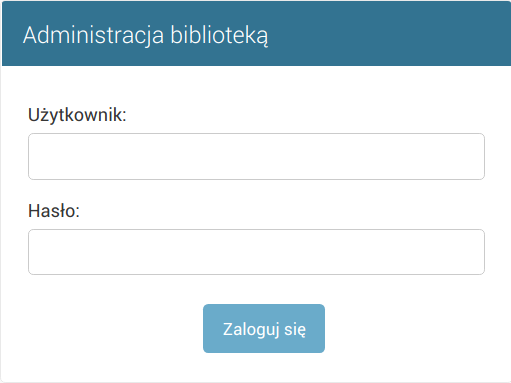
\includegraphics[width=0.6\linewidth]{img/backend/oknLogowania.png}
  \caption{Okno logowania do panelu administracyjnego}
  \label{fig:adminLogin}
\end{figure}

Po zalogowaniu powinien się ukazać panel administracyjny do zarządzania biblioteką (rysunek \ref{fig:adminPanel}). 

W nagłówku strony zatytułowanym ,,Administracja biblioteką'', znajduje się dwa odnośniki. Pierwszy daje możliwość zmiany hasło do konta, drugi wylogowuje obecnego użytkownika. Poniżej nagłówka znajdują się dwie sekcje zatytułowane ,,Biblioteka'' oraz ,,Uwierzytelnianie i Autoryzacja'', które zostały opisane w kolejnych rozdziałach. Po prawej stronie sekcja ,,Ostatnie działania'', wyświetająca listę ostatnich zmian wprowadzonych w aplikacji.


\begin{figure}[h]
  \centering
  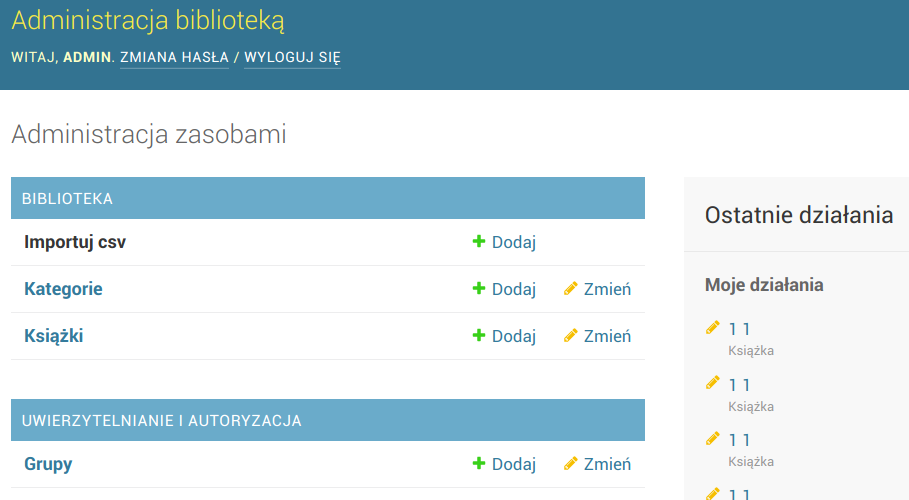
\includegraphics[width=0.6\linewidth]{img/backend/PanelAdmin.png}
  \caption{Strona główna panelu administracyjnego}
  \label{fig:adminPanel}
\end{figure}

\subsection{Biblioteka}
W skad tej sekcji wchodzą opcje importowania plików \verb`*.csv`, zarządzania kategoriami oraz zarządzania książkami.

\begin{figure}[h]
  \centering
  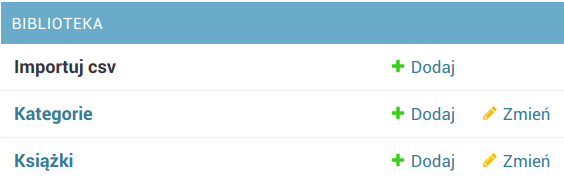
\includegraphics[width=0.6\linewidth]{img/backend/biblioteka.png}
  \caption{Sekcja "Biblioteka"}
  \label{fig:biblioteka}
\end{figure}

\subsubsection{Importuj csv}
Po naciśnięciu ,,+ Dodaj'', w wierszu ,,Importuj csv'' (rysunek \ref{fig:biblioteka}), otworzy się panel zatytułowany ,,Dodaj CSV'', widoczny na rysunku \ref{fig:importCSV}. Aby wczytać plik CSV, należy wskazać jego lokalizację (klikając przycisk ,,Wybierz plik'') a następnie kliknąć przycisk ,,Zapisz''. Po załadowaniu danych z pliku CSV wyświetli się lista komunikatów dotycząca statusu importowanych danych. 

\begin{figure}[h]
  \centering
  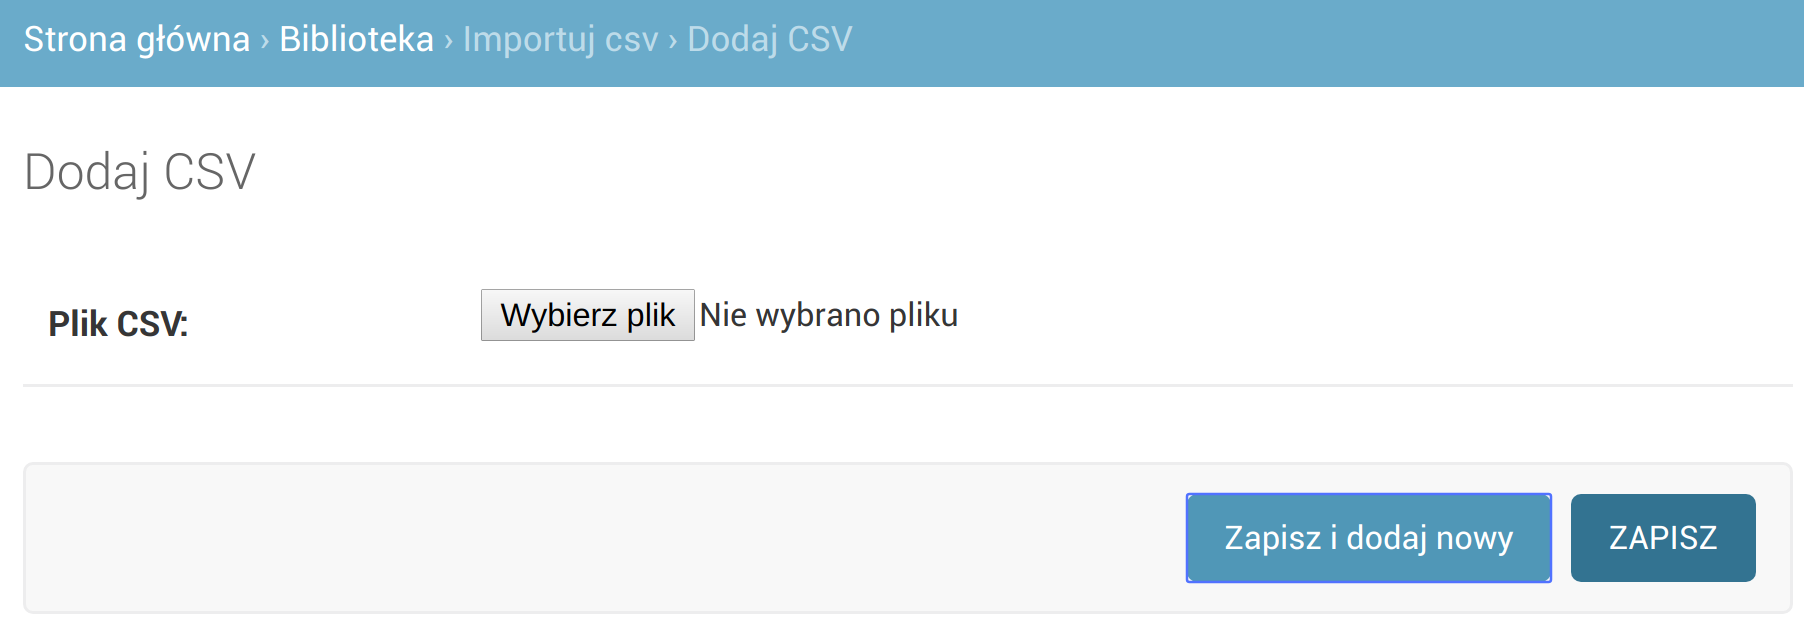
\includegraphics[width=0.6\linewidth]{img/backend/ImportCSV.png}
  \caption{Formularz importowania plików *.csv}
  \label{fig:importCSV}
\end{figure}


Pliki \verb`*.csv` powinny zostać wygenerowane na podstawie arkusza kalkulacyjnego \verb`dane-prog-bibl.xlsx`, kodowanie pliku to UTF-8, symbol oddzielający pola to \textbf{,} a separator tekstu to symbol \textbf{"}. Aplikacja sama rospoznaje czy importowany plik \verb`*.csv` zawiera informacje z zakładki KSIAZKA, KATEGORIE czy PRZYPISANIE\_KATEGORII.

\subsubsection{Kategorie}

Wybór ,,Kategorie'' w sekcji ,,Biblioteka'' (rysunek \ref{fig:biblioteka}), przenosi do widoku z listą wszystkich kategorii, widocznego na rysunku \ref{fig:adminAllCategories}. Z poziomu tej listy można usuwać wybrane kategorie oraz wyszukiwać kategorie wpisując w pole tekstowe części id kategorii lub nazwy kategorii. Klikając na id kategorii w liście, otworzy się formularz edycji danej kategorii, widoczny na rysunku \ref{fig:adminEditCategory}. 

\begin{figure}[h]
  \centering
  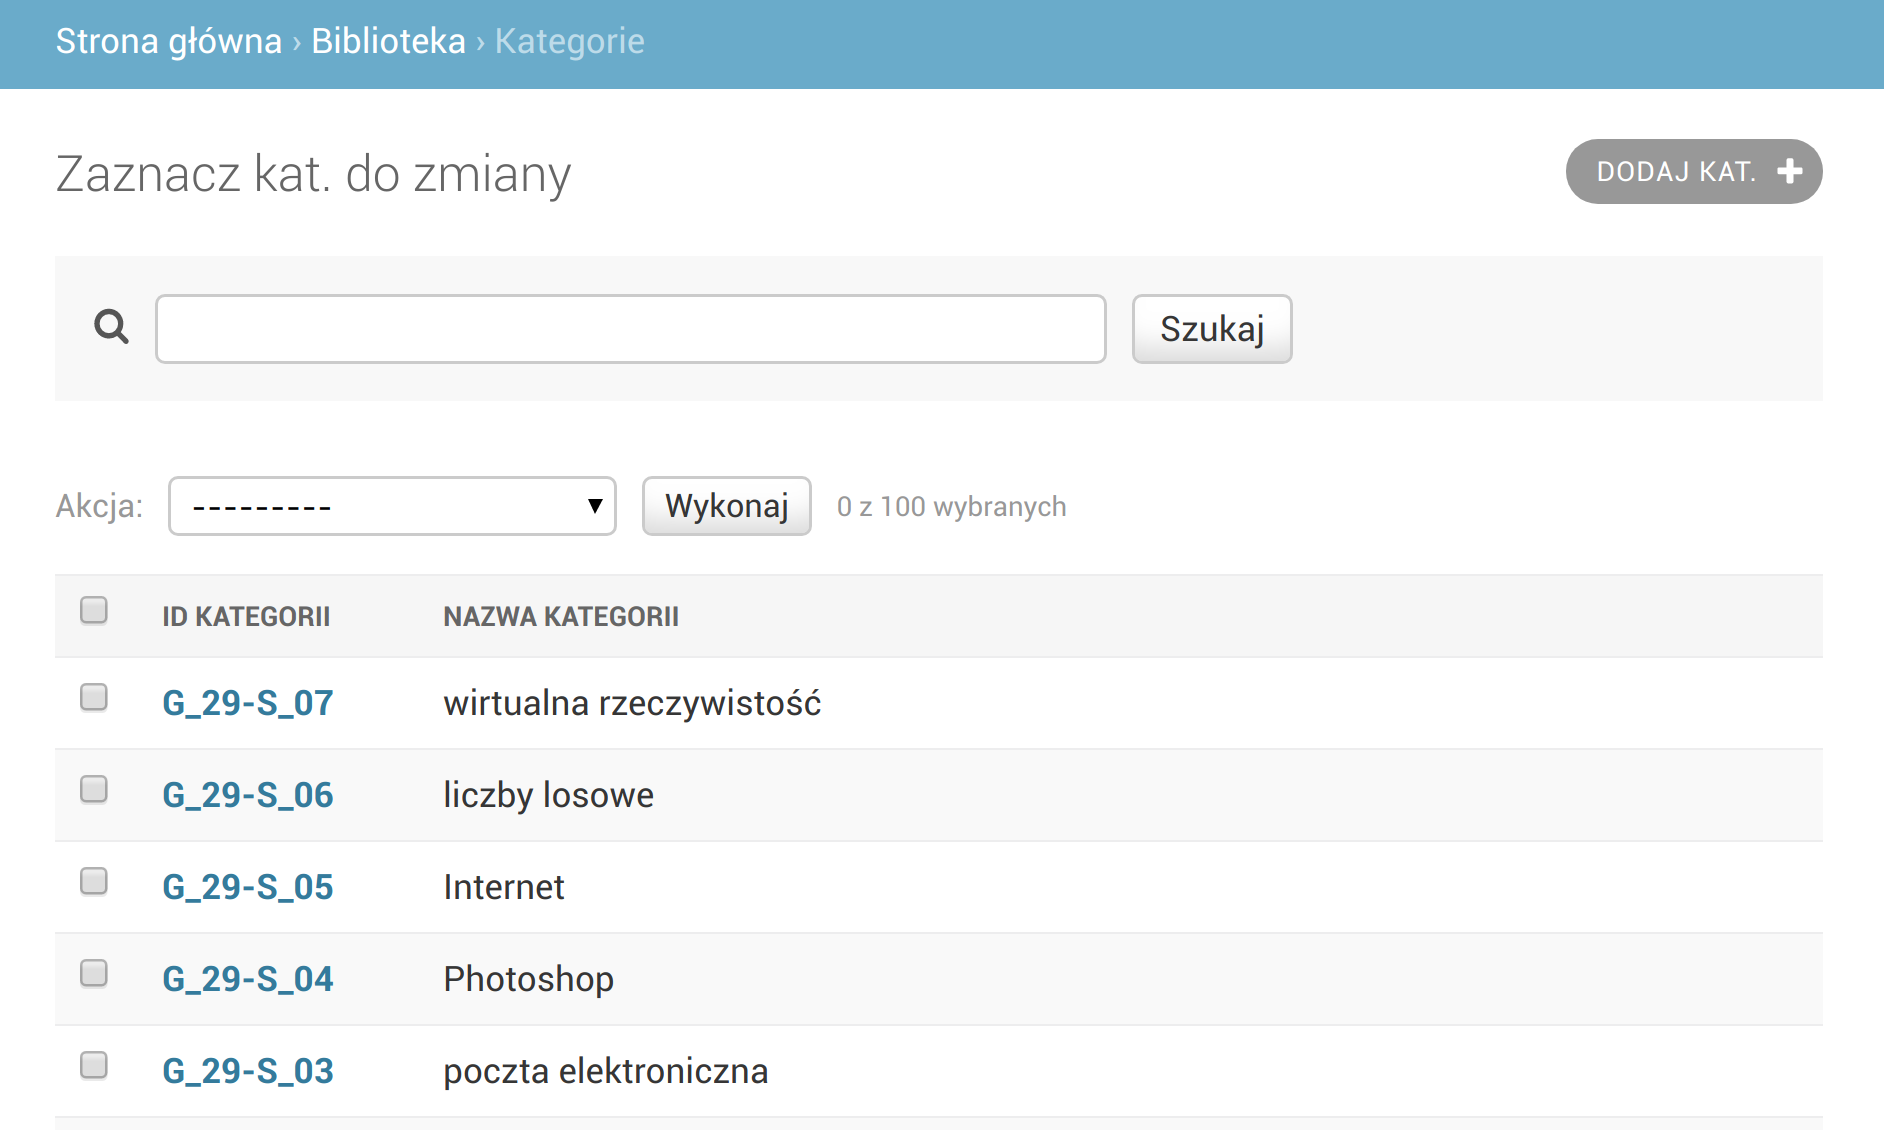
\includegraphics[width=0.6\linewidth]{img/backend/ListaKategorii.png}
  \caption{Widok listy kategorii}
  \label{fig:adminAllCategories}
\end{figure}

Po naciśnieciu ,,Dodaj kat. +'' (prawy górny róg na rysunku \ref{fig:adminAllCategories}), otworzy się formularz tworzenia nowej kategorii. Aby dodać kategorię główną nadajemy jej id \verb`G_nr_kat`, gdzie \verb`nr_kat` to ciąg cyfr. Aby dodać kategorię szczegółową nadajemy jej id \verb`G_nr_kat-S_nr_sub_kat`, gdzie \verb`G_nr_kat` to id kategorii głównej, a \verb`nr_sub_kat` to id kategorii szczegółowej.
Z poziomu okna edycji kategorii można podejrzeć historię naniesionych zmian wybierając ,,Historia'' (prawy górny róg rysunku \ref{fig:adminEditCategory}).



\begin{figure}[h]
  \centering
  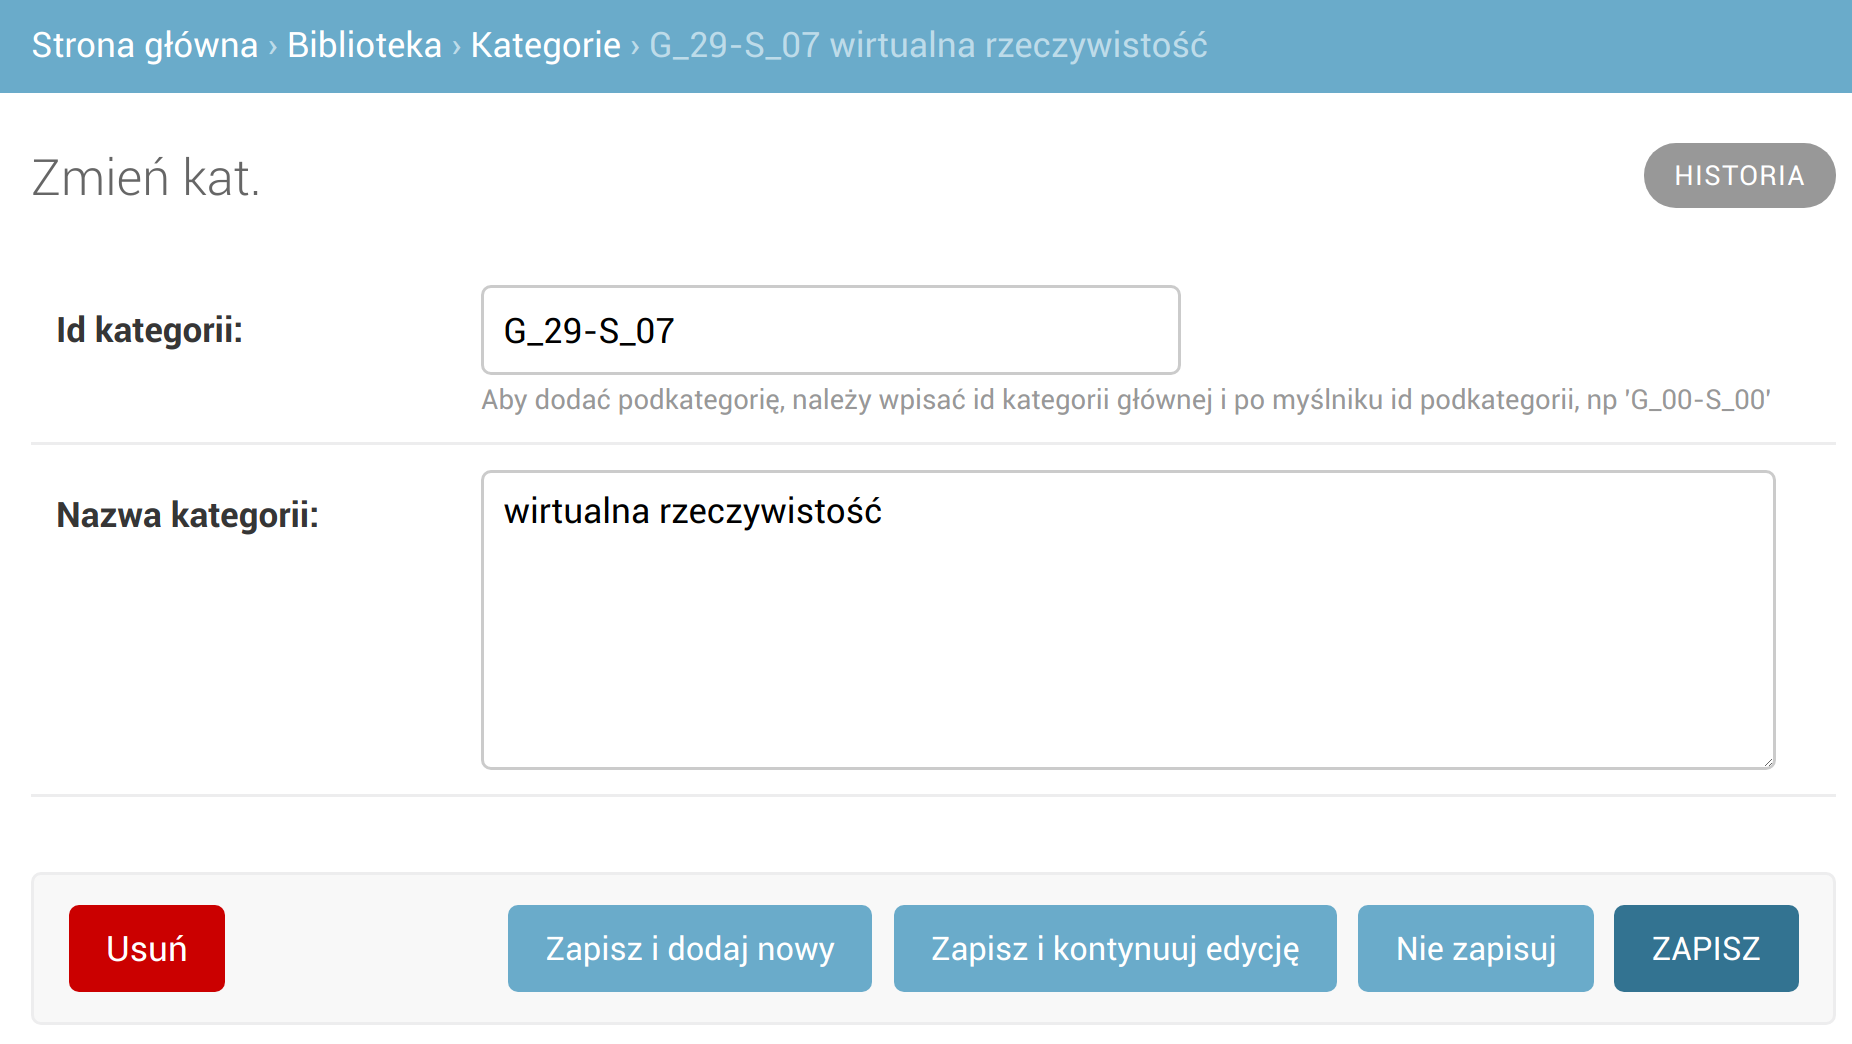
\includegraphics[width=0.6\linewidth]{img/backend/EdycjaKategorii.png}
  \caption{Formularz edycji kategorii}
  \label{fig:adminEditCategory}
\end{figure}

\subsubsection{Książki}

Po naciśnieciu ,,Książki'' w sekcji ,,Biblioteka'' (rysunek \ref{fig:biblioteka}), otworzy się widok z~listą książek, widoczny na rysunku \ref{fig:adminBooks}. 

\begin{figure}[h]
  \centering
  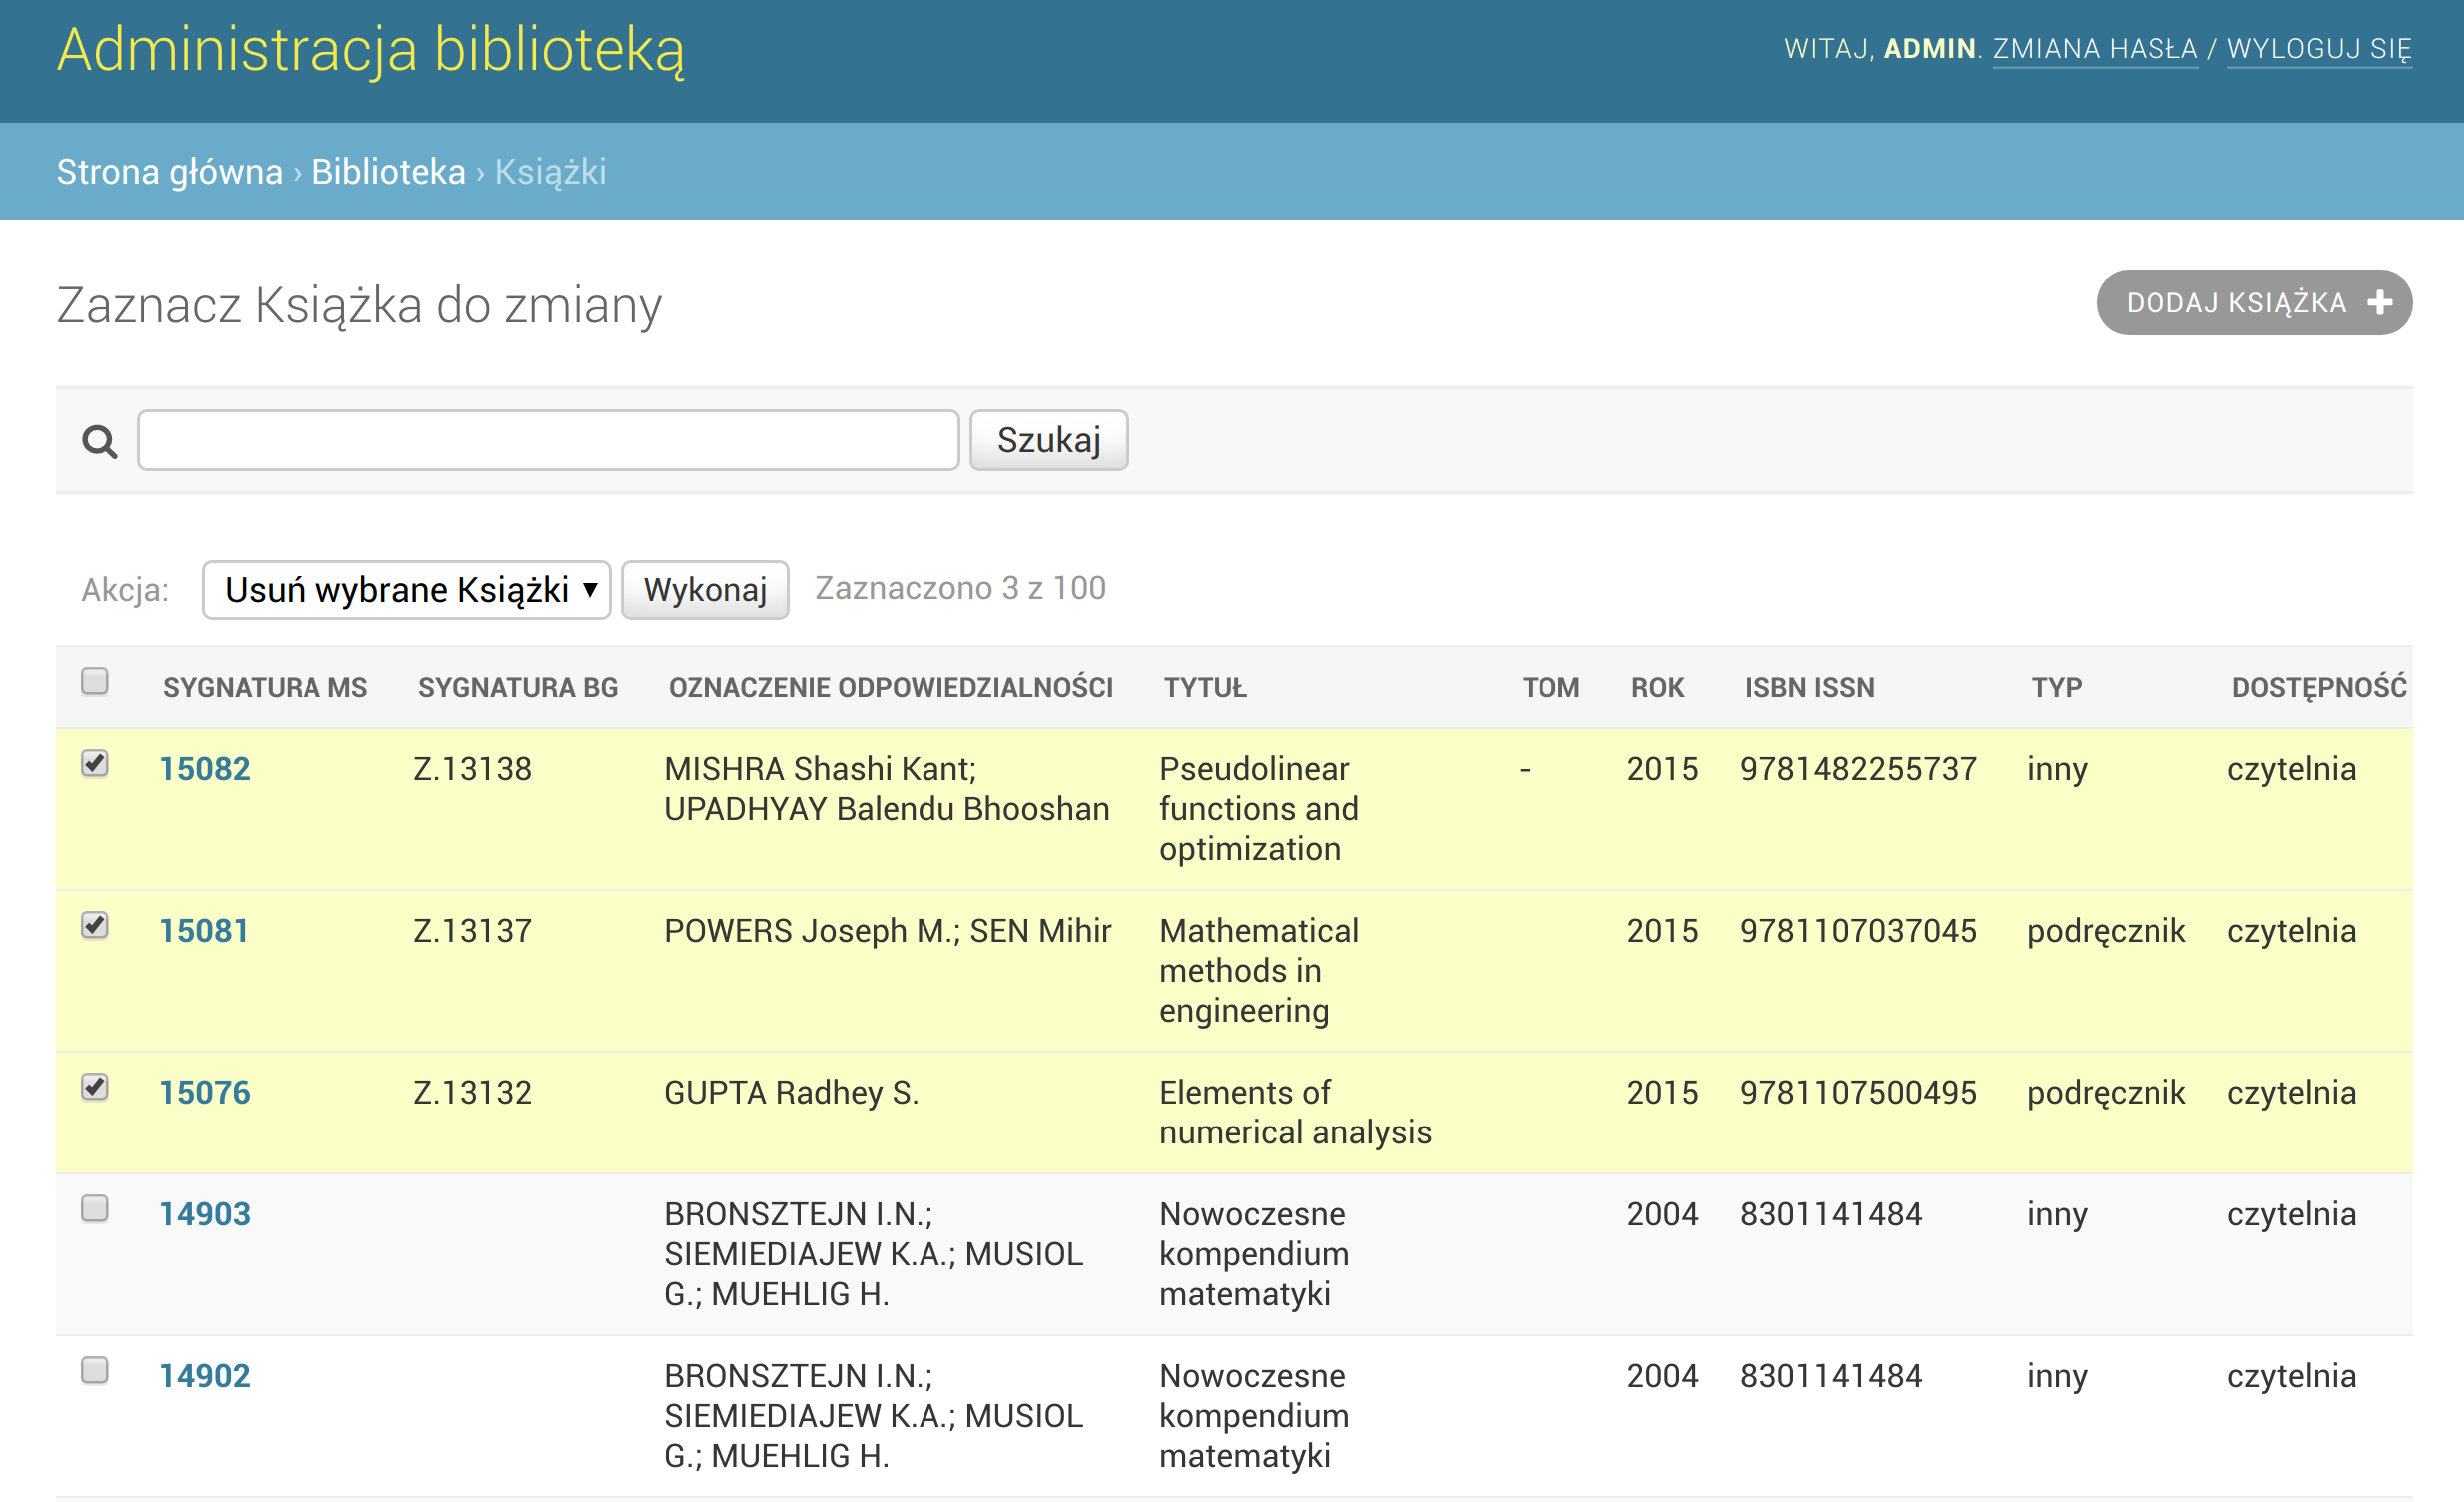
\includegraphics[width=0.6\linewidth]{img/backend/ListaKsiazek.png}
  \caption{Widok listy książek}
  \label{fig:adminBooks}
\end{figure}

Z poziomu widoku z listą można:
\begin{itemize}
	\item wyszukać książkę, wpisując jej id (całe) lub fragment tytułu,
	\item sortować wyświetlone książki po dowolnym zbiorze pól, klikając na nazwę tych pól w nagłówku tablicy, w odpowiedniej kolejności,
	\item usuwać wybrane książki, poprzez zaznaczenie zbioru książek i wykonanie akcji ,,Usuń wybrane Książki'',
	\item wybrać książkę do edycji, klikając jej id na liście,
	\item dodać nową książkę, klikając ,,Dodaj Książka +''.
\end{itemize}

Po wybraniu książki do edycji, otworzy się fromularz edycji książki widoczny na rysunku \ref{fig:adminEditBook}.

\begin{figure}[h]
  \centering
  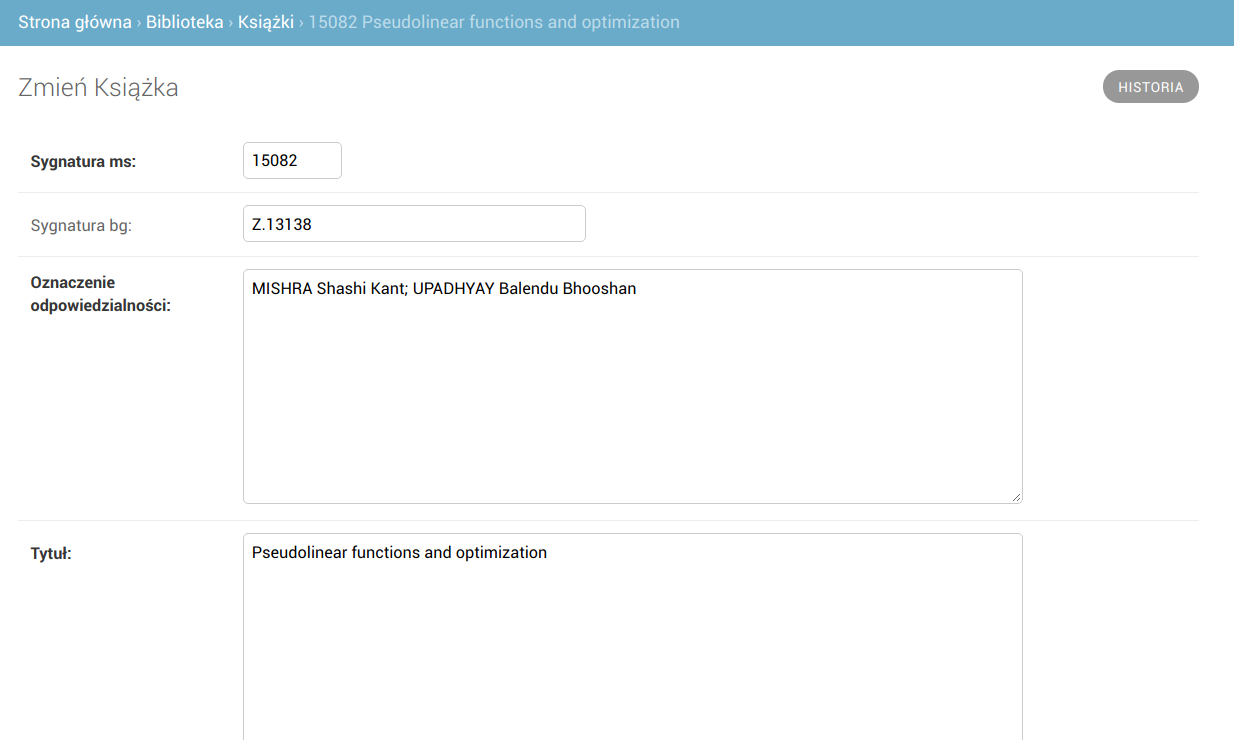
\includegraphics[width=0.6\linewidth]{img/backend/EdycjaKsiazki.png}
  \caption{Formularz edycji książki}
  \label{fig:adminEditBook}
\end{figure}

Z poziomu okna edycji książki można przejrzeć historię naniesionych zmian wybierając ,,Historia''. Widok zmian widoczny na rysunku \ref{fig:adminBookHistory}.

\begin{figure}[h]
  \centering
  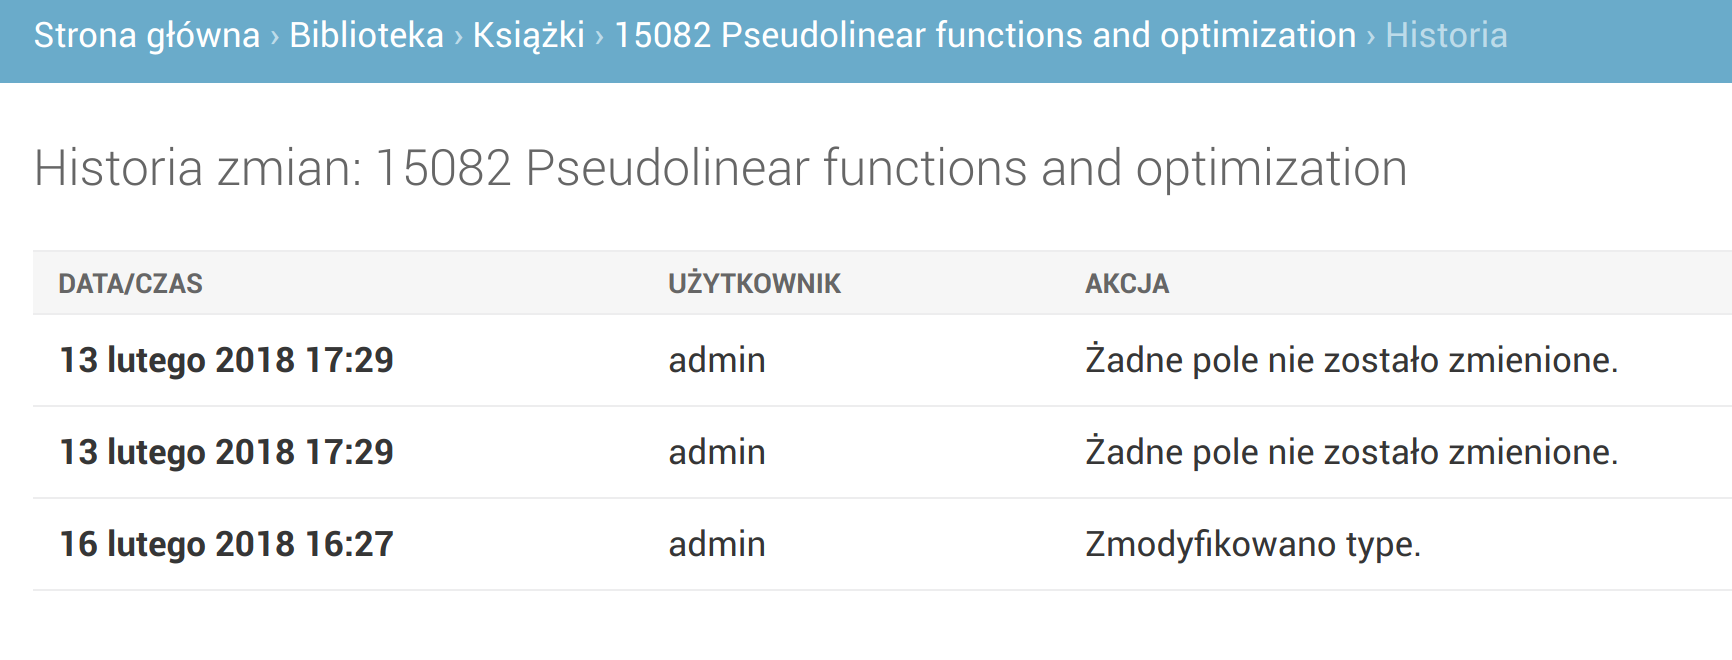
\includegraphics[width=0.6\linewidth]{img/backend/HistoriaZmian.png}
  \caption{Widok historii zmian książki}
  \label{fig:adminBookHistory}
\end{figure}


\subsection{Uwierzytelnianie i Autoryzacja}
Sekcja ta składa się z opcji tworzenia i zarządzania kontami użytkowników i grup użytkowników.

\begin{figure}[h]
  \centering
  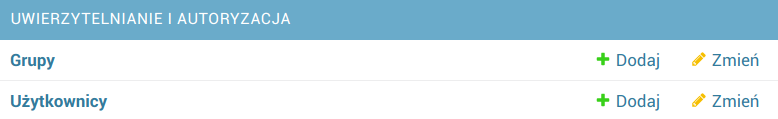
\includegraphics[width=0.6\linewidth]{img/backend/autoryzacja.png}
  \caption{Sekcja ,,Uwierzytelnianie i Autoryzacja''}
  \label{fig:authSection}
\end{figure}

Obecnie aplikacja nie wykorzystuje grup użytkowników, opcja ta została jednak pozostawiona gdyby w przyszłości projekt miał zawierać konta studentów z możliwością rezerwacji książek.
 
W celu dodania nowego konto administratora biblioteki należy wybrać opcję ,,+ Dodaj'', znajdującą się w wierszu ,,Użytkownicy'' (rysunek \ref{fig:authSection}). Następnie zostanie otwarty formularz widoczny na rysunku \ref{fig:newUserForm}. Należy go wypełnić i~zapisać.

\begin{figure}[h]
  \centering
  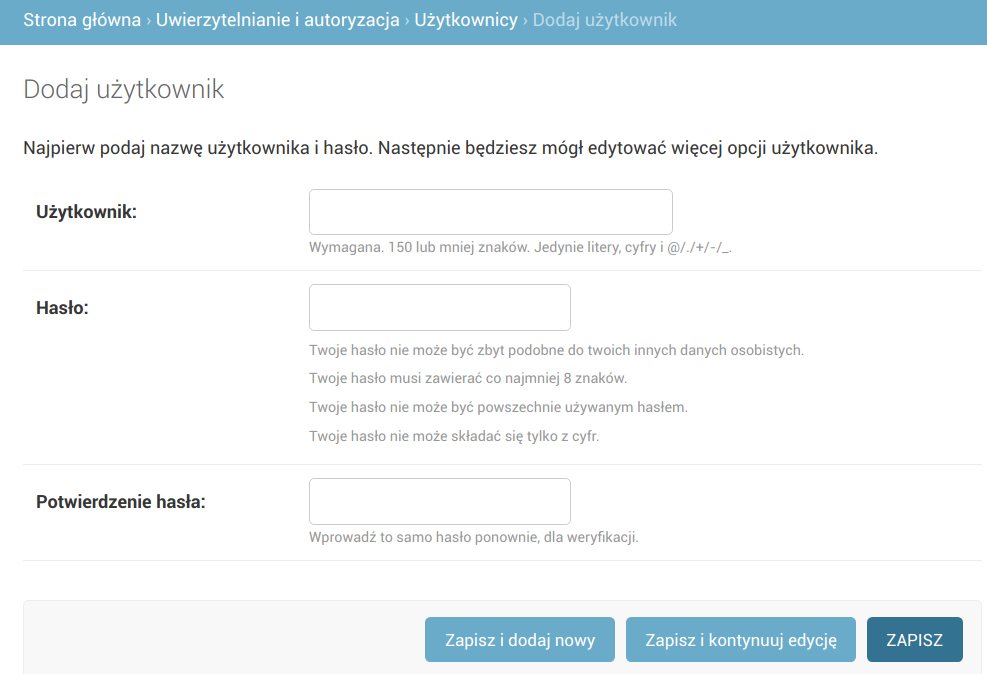
\includegraphics[width=0.6\linewidth]{img/backend/NowyAdminForm.png}
  \caption{Formularz nowego użytkownika}
  \label{fig:newUserForm}
\end{figure}

Nowy użytkownik powinien się teraz pojawić na liście wszystkich użytkowników aplikacji. Aby nadać mu uprawnienia administracyjne, należy wybrać na liście (widocznej na rysunku \ref{fig:usersList}) nowo dodanego użytkownika.

\begin{figure}[h]
  \centering
  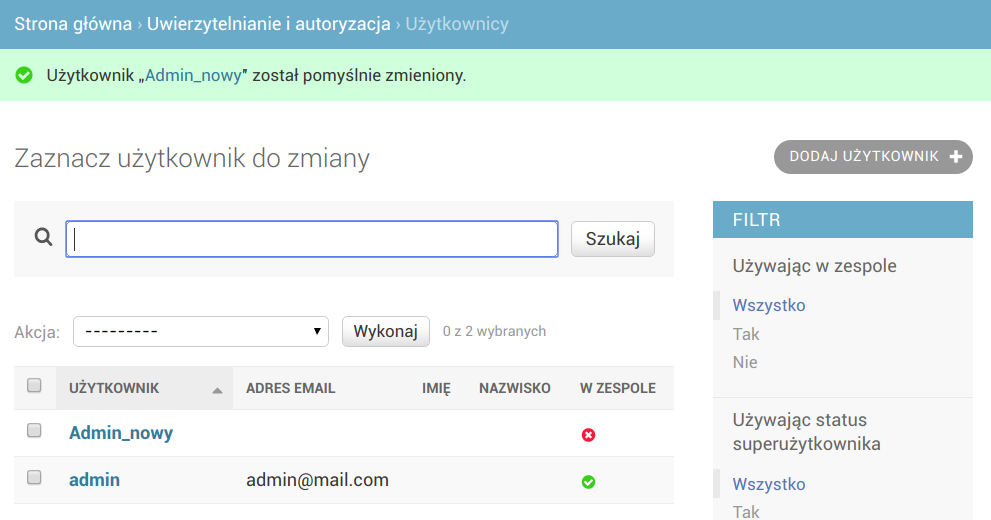
\includegraphics[width=0.6\linewidth]{img/backend/ListaUser.png}
  \caption{Lista użytkowników aplikacji}
  \label{fig:usersList}
\end{figure}

W formularzu edycji nowego użytkownika (rysunek \ref{fig:editUser}), w sekcji ,,Uprawnienia'', należy zaznaczyć opcję ,,W zespole'' i zapisać.

\begin{figure}[h]
  \centering
  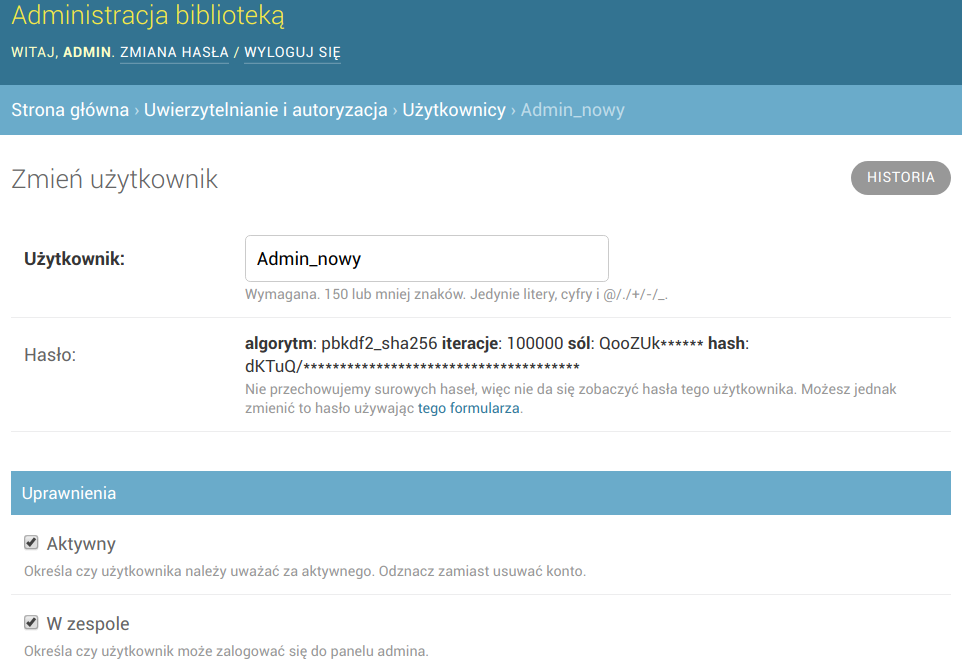
\includegraphics[width=0.6\linewidth]{img/backend/Uprawnienia.png}
  \caption{Formularz edycji użytkownika}
  \label{fig:editUser}
\end{figure}

\section{Aplikacja na system Android}

\subsection{Wykorzystane narzędzie}

Aplikacja na urządzenia mobilne z systemem Android została napisana w języku \textit{Java 8} w programie \textit{Android Studio} w wersji $3.0.1$.

\textit{Java} jest uniwersalnym językiem obiektowym stworzonym w 1996 roku przez Jamesa Goslinga, Billy'ego Joya oraz Guya Steele \cite{javaOracle}. Cechuje go prostota, celem twórców było, aby każdy mógł z łatwością osiągnąć płynność w korzystaniu z \textit{Javy}. Jest mocno powiązana z językami programowania \textit{C} oraz \textit{C++} \cite{javaOracle}. 

\textit{AndroidStudio} jest oficjalnym środowiskiem programistycznym do tworzenia aplikacji na system Android, ogłoszonym w 2013 roku przez Google \cite{PPPAndroida}. Wersja $3.0.1$ weszła w życie w październiku 2017 roku wprowadzając, między innymi, wsparcie najnowszej wersji Android $8$ \cite{androidStudioDev}. Widać, że do tworzenia aplikacji mobilnej zostały wybrane najnowsze i jedne z najbardziej znanych narzędzi.
 
\subsection{Wymagania systemowe}

Aplikację można zainstalować na telefonach komórkowych oraz tabletach z systemem Android w wersji minimum $5.0$ Lollipop (API $21$). Według statystyk z dnia $5$ lutego $2018$ roku \cite{androidStatistics} przedstawionych na rysunku \ref{fig:androidStats} najwięcej użytkowników korzysta z wersji Marshmallow $6.0$. Jednak duży procent nadal używa wersji Lollipop, nie jest to na tyle znacząca różnica, aby zignorować tę wersję. Aplikację będzie mogło używać około $24\%$ więcej użytkowników.    

\begin{figure}[h]
  \centering
  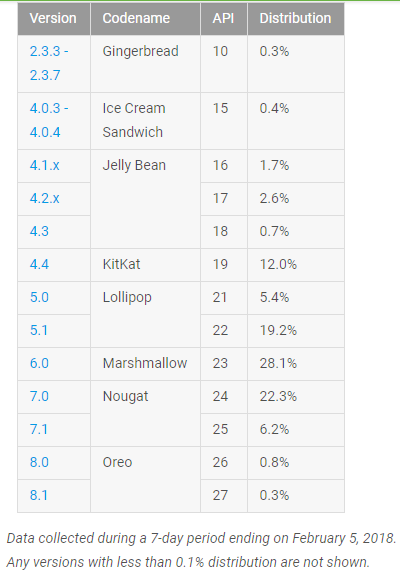
\includegraphics[width=0.6\linewidth]{img/android/stats.png}
  \caption{Procent urządzeń z uruchomioną daną wersją Androida}
  \label{fig:androidStats}
\end{figure}

\subsection{Model danych}
Aplikacja posiada następujący model danych stworzony na podstawie informacji dostarczanych z API:

\begin{itemize}
\item \verb`Book` -- klasa reprezentująca obiekt książki:
\begin{itemize}
\item \verb`title` (\verb`String`) -- tytuł,
\item \verb`responsibility` (\verb`String`) -- autorzy,
\item \verb`year` (\verb`Integer`) -- rok wydania,
\item \verb`volume` (\verb`String`) -- tom,
\item \verb`availability` (\verb`String`) -- dostępność,
\item \verb`type` (\verb`String`) -- typ pozycji,
\item \verb`isbnWithIssn` (\verb`String`) -- numer ISBN/ISSN,
\item \verb`facultySignature` (\verb`String`) -- sygnatura biblioteki MS,
\item \verb`mainSignature` (\verb`String`) -- sygnatura biblioteki głównej,
\item \verb`categories` (\verb`List<Category>`) -- kategorie przypisane do książki.
\end{itemize}
\item \verb`CategoryResponse` -- klasa reprezentująca kategorie:
\begin{itemize}
\item \verb`category` (\verb`Category`) -- kategoria,
\item \verb`subcategories` (\verb`List<Category>`) -- podkategorie przypisane do kategorii.
\end{itemize}
\item \verb`Category` -- klasa reprezentująca obiekt kategorii:
\begin{itemize}
\item \verb`categoryId` (\verb`String`) -- id kategorii,
\item \verb`name` (\verb`String`) -- nazwa kategorii.
\end{itemize}
\item \verb`Dictionary` -- klasa reprezentująca obiekt "słownik" dla książki:
\begin{itemize}
\item \verb`bookTypes` (\verb`String[]`) -- typy pozycji (podręcznik, zbiór zadań, inny),
\item \verb`bookAvailabilities` (\verb`String[]`) -- dostępność (dostępna, wypożyczona, czytelnia).
\end{itemize}
\end{itemize}


\subsection{Realizacja projektu}

Poniższe rozdziały opisują budowę poszczególnych obiektów klasy \verb`Activity`, które w dalszej części pracy będą nazywane aktywnościami. 

W celu monitorowania działania aplikacji po wdrożeniu, został do niej przyłączony \textit{Crashlytics} \cite{crashlytics}. Jest to jedno z najlepszych urządzeń, które pozwala na śledzenie działania aplikacji. Biblioteka ta jest częścią platformy \textit{Fabric}. Poza analizą ilości użytkowników w danych okresie czasu, pozwala na bieżąco śledzić błędy krytyczne powodujące zatrzymanie działania aplikacji. System Android jest jednym z najbardziej znanych i najczęściej używanych systemów, co niestety rodzi pewne problemy. Na przykład ilość urządzeń oraz ich różnorodność. Aplikacja wspiera cztery główne wersje systemu oraz wszystkie rozmiary telefonów i tabletów. Bardzo trudno jest dobrze przetestować taki produkt i znaleźć wszystkie możliwe niepożądane działania. Stąd pomysł na wprowadzenie Crashlyticsa. W każdej chwili można sprawdzić na stronie \href{https://fabric.io/}{fabric.io} raport błędów wysłany przez bibliotekę. Między innymi zostają wyświetlone data, czas i ilość wystąpień konkretnego błędu, model urządzenia oraz wersja Androida, na którym wybrany błąd się pojawił, a także sam log błędu. 

\subsubsection{ModelViewPresenter}

Projekt powstał w oparciu o strukturę \textit{Model View Presenter}. \textit{MVP} jest wzorcem projektowym stworzonym na podstawie wzorca \textit{Model View Controller}. Podobnie jak w \textit{MVC}, \textit{Model} odpowiada za reprezentację obiektów danych, a \textit{View} za wyświetlanie informacji użytkownikowi. Presenter natomiast jest odpowiedzialny za odseparowanie modelu od widoku. Podejmuje decyzję o tym, co powinno być wyświetlone użytkownikowi. Na podstawie dostarczonych danych przez \textit{Model}, zwraca je w reprezentacyjnej formie do \textit{View}. W przeciwieństwie do \textit{Controllera} z \textit{MVC}, nie posiada w sobie żadnych elementów \textit{UI} \cite{mvpBook}. Rysunek \ref{fig:mvp} przedstawia uproszczony model \textit{MVP}.

\begin{figure}[h]
  \centering
  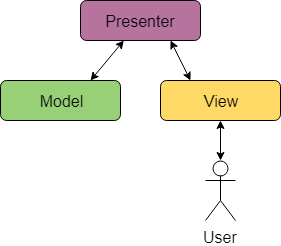
\includegraphics[width=0.5\linewidth]{img/android/mvp.png}
  \caption{Związek między odpowiednimi elementami \textit{MVP}}
  \label{fig:mvp}
\end{figure}

W projekcie \textit{Model} został odseparowany przez przeniesienie wszystkich klas związanych z pobieraniem/wysyłaniem danych do paczki \verb`data`, co widać na rysunku \ref{fig:mvpProject}. Natomiast elementy widoku znajdują się w paczce \verb`ui`. W nich występuje również konkretny podział na klasy \textit{View} oraz \textit{Presenter}. Dodatkowo występuje tu interfejs \verb`Contract`, który łączy w sobie interfejsy \textit{Presentera} i \textit{View}. Użycie interfejsów umożliwia zarządzanie widokiem z poziomu \textit{Presentera}, bez konieczności posiadania elementów widoku w nim. 

\begin{figure}[h]
  \centering
  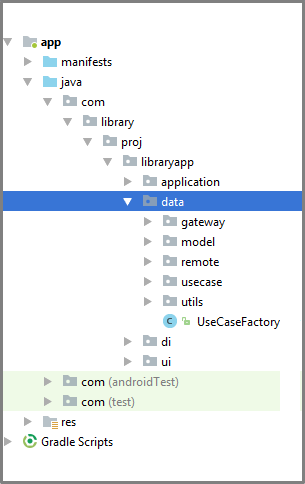
\includegraphics[width=0.4\linewidth]{img/android/mvpData.png}
  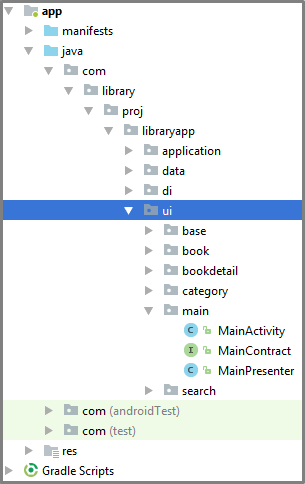
\includegraphics[width=0.4\linewidth]{img/android/mvpMainActivity.png}
  \caption{Podział projektu z uwzględnieniem struktury \textit{MVP}}
  \label{fig:mvpProject}
\end{figure}

W celu uproszczenia i polepszenia czytelności kodu w projekcie została również użyta biblioteka \textit{Dagger2} \cite{dagger2}.
Jest to implementacja wzorca \textit{Dependency Injection}, czyli wstrzykiwania zależności. Celem tego podejścia jest minimalizacja tworzenia obiektów poprzez 
\begin{verbatim}
new ClassName()
\end{verbatim}
oraz stworzenie repozytorium obiektów, które możemy wstrzyknąć w
dowolnym miejscu aplikacji \cite{PPPAndroida}.

\subsubsection{Pobieranie i wysyłanie danych}

Do pobierania i wysyłania danych oraz łączenia się z serwerem wykorzystano biblioteki \textit{Retrofit} \cite{retrofit} oraz \textit{RxJava2} \cite{rxjava2}.

\textit{Retrofit} jest darmową biblioteką przeznaczoną do korzystania z API REST z~poziomu Androida. Dzięki metodom oraz anotacjom zawartym w bibliotece budowanie zapytań jest szybkie, proste i przede wszystkim przejrzyste (rysunek \ref{fig:retrofit}). Jej ogromną zaletą jest również wbudowana obsługa GSON, która zapewnia automatyczne mapowanie obiektów POJO na JSON i odwrotnie \cite{PPPAndroida}.

\begin{figure}[h]
  \centering
  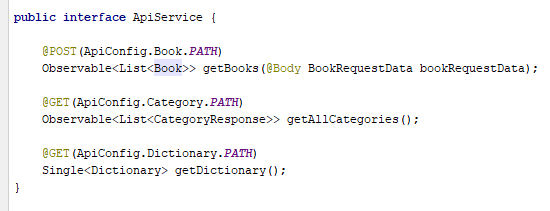
\includegraphics[width=0.8\linewidth]{img/android/apiService.png}
  \caption{Fragment klasy \textit{ApiService} zawierającej metody pobrania książek, kategorii oraz słownika z API}
  \label{fig:retrofit}
\end{figure}

Natomiast biblioteka \textit{RxJava} rozszerza wzorzec \textit{Observable}, w celu umożliwienia prostej obsługi sekwencji danych/zdarzeń. Umożliwia odpowiednie składanie sekwencji, jednocześnie eliminując możliwe błędy związane ze złą synchronizacją zdarzeń oraz działaniem na wielu wątkach \cite{rxjava2}.

\subsubsection{Zarządzanie widokami}

Widoki zostały stworzone w plikach z rozszerzeniem \verb`xml`. Przekazanie ich do klas zarządzającymi aktywnościami odbyło się z użyciem biblioteki \textit{ButterKnife} \cite{butterknife}. Jest to bardzo prosta, darmowa biblioteka, która generuje kod związany z dostępem do UI na podstawie anotacji \cite{PPPAndroida}. Dzięki niej łatwiej jest dbać o czystość kodu, niepotrzebne jest używanie \verb`findViewById`, a podpięcie listenerów zajmuje mniej miejsca i jest bardziej czytelne, co widać na obrazku \ref{fig:butterknife}.

\begin{figure}[h]
  \centering
  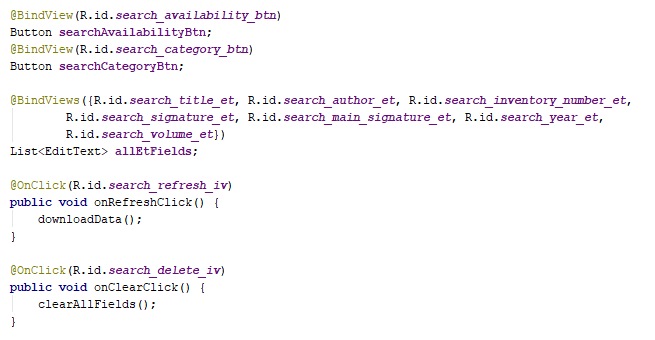
\includegraphics[width=0.85\linewidth]{img/android/butterknife.png}
  \caption{Przykład zastosowania biblioteki \textit{ButterKnife} w klasie \textit{SearchActivity}}
  \label{fig:butterknife}
\end{figure}

\subsubsection{BaseActivity}

Pierwszą, a zarazem najważniejszą klasą obiektu \verb`Activity` jest klasa abstrakcyjna \verb`BaseActivity`, którą wszystkie pozostałe aktywności rozszerzają. W całej paczce \verb`base` znajdują się także interfejs \verb`BaseView`, który aktywność implementuje oraz interfejs i klasę \verb'Presenter'. Jest to zbiór podstawowych klas i interfejsów, które kolejne klasy będą rozszerzać bądź implementować. Poza podstawowymi metodami, takimi jak:
\begin{verbatim}
getLayoutRes();
performFieldInjection(ActivityComponent activityComponent);
getActivityComponent();
\end{verbatim} 
które przypominają o konieczności wstrzyknięcia instancji klasy do prezentera, została zaimplementowana również poniższa metoda:
\begin{verbatim} 
final void onDetachView() {
    view = null;
    if(compositeDisposable != null 
        && !compositeDisposable.isDisposed()) {
        compositeDisposable.dispose();
    }
}
\end{verbatim}

Jej celem jest przerwanie wszystkich połączeń z API, gdy widok zostanie zniszczony, na przykład w przypadku, gdy użytkownik wyłączy aplikację.

\subsubsection{MainActivity}

Celem \verb`MainActivity` jest wyświetlenie powitalnego ekranu użytkownikowi, tak zwanego \textit{SplashScreena}, który po $1.5$ sekundy znika i otwiera widok wyszukiwania. W przyszłości w tym miejscu można dodać opcję logowania lub utworzenia nowego konta do aplikacji.

Cały widok, podobnie jak pozostałe, zawiera się w \verb`ConstraintLayout` \cite{constraintLayout}. Jest to jeden z najnowszych obiektów typu \verb`ViewGroup` wprowadzony razem z wersją $3.0$ Android Studio. Do tej pory najczęściej używanymi elementami były \verb`RelativeLayout` oraz \verb`LinearLayout`, które działają prosto i intuicyjnie, ale mimo wszystko są mocno ograniczone. \verb`ConstraintLayout` jest stworzony przede wszystkim do ułatwienia tworzenia widoków przy pomocy wbudowanego narzędzia \textit{Layout Editor's}. Umożliwia tworzenie pojedynczych widoków, z których każdą krawędź można pozycjonować względem dowolnie wybranych innych elementów znajdujących się w grupie. Następnie umożliwia tworzenie łańcuchów widoków i pozycjonowanie ich tak, jakby były jednym obiektem, bez konieczności dodawania i zagnieżdżania kolejnego obiektu typu \verb`ViewGroup`. 

\subsubsection{SearchActivity}

Jest to aktywność otwierana bezpośrednio z poprzedniej, po upływie danego czasu. 

\begin{figure}[h]
  \centering
  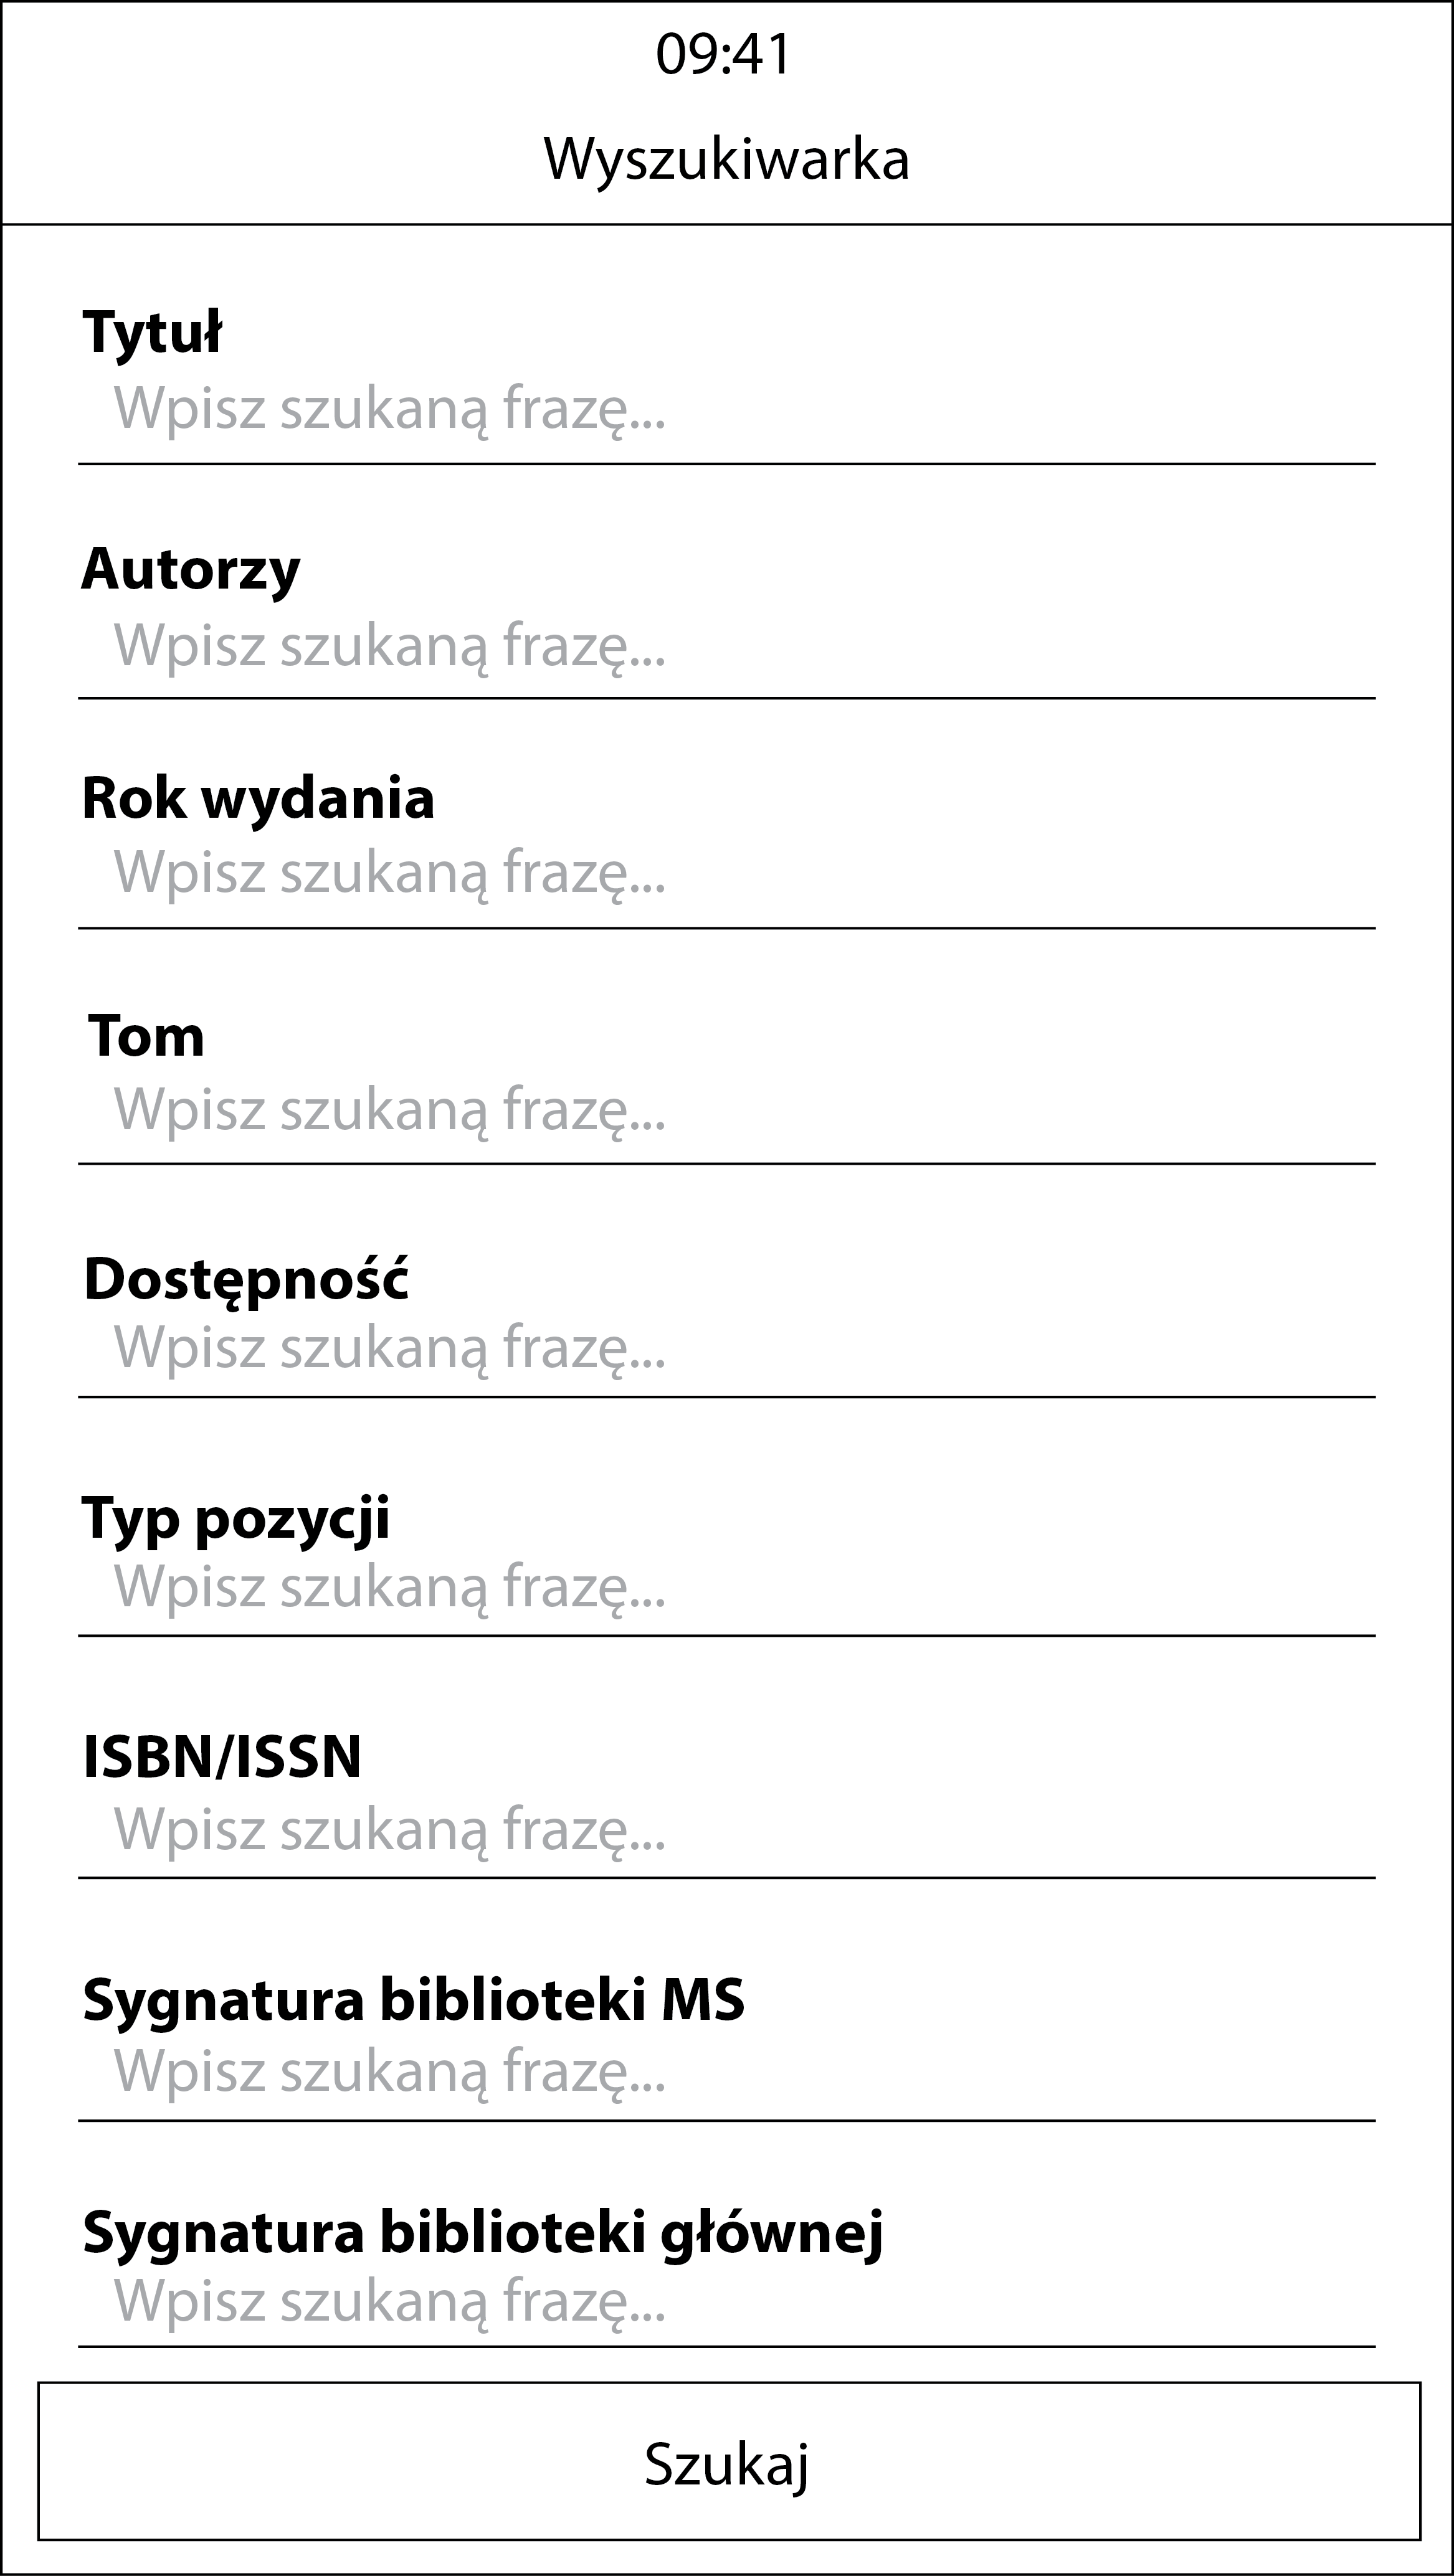
\includegraphics[width=0.4\linewidth]{img/SearchProject.png}
  \caption{Projekt ekranu wyszukiwania książek}
  \label{fig:androidSearch}
\end{figure}

Jej celem jest umożliwienie wprowadzenia filtrów szukanych książek przez użytkownika. Widok składa się z customowego elementu typu \verb`Toolbar`, elementów typu  \verb`TextInputEditText`, w które użytkownik może wprowadzić tekst oraz obiektów \verb`Button` widocznych na wstępnym projekcie \ref{fig:androidSearch}.

\verb`Toolbar` został dodany w celu poprawienia czytelności aplikacji, zwiększenia intuicyjnego działania oraz ułatwienia nawigacji pomiędzy widokami. Każda aktywność posiada swój \verb`Toolbar`. W przypadku \verb`SearchActivity` znajduje się tam tekst z informacją, na którym widoku znajduje się użytkownik, po lewej stronie ikona do odświeżenia informacji przychodzących z API (np. typ, dostępność książki oraz kategorie w przypadku braku internetu nie zostaną pobrane), po prawej ikona usunięcia wszystkich, do tej pory, wprowadzonych danych. 

Obiekt \verb`TextInputEditText` \cite{textInputEditText} jest podklasą obiektu \verb`EditText`. Różni się od tradycyjnego wejściowego pola tekstowego tym, że w momencie pisania oraz po wprowadzeniu tekstu przez użytkownika powyżej, mniejszą czcionką znajduje się podpowiedź, która wcześniej była wyświetlana. W tym wypadku jest to informacja, co należy w dane pole wpisać.

Filtry takie jak dostępność książki, typ pozycji oraz kategorię można wybrać po naciśnięciu obiektu \verb`Button`. W przypadku dwóch pierwszych zostanie wyświetlony \verb`Dialog` z listą możliwości do wyboru. W klasie odpowiedzialnej za tworzenie odpowiedniego dialogu znajduje się interfejs, dzięki któremu w łatwy sposób następuje przekazanie wybranych elementów do aktywności.
\begin{verbatim}
public interface OnDictionaryDialogResult {
    void finish(String selectedItem);
}
\end{verbatim} 

Po naciśnięciu na element z listy następuje wywołanie metody \verb`finish()` zaimplementowanej w aktywności.
\begin{verbatim}
adapter.getOnDictionaryItemClickSubject().subscribe(
        dictionary -> {
            onDictionaryDialogResult.finish(dictionary);
            dismiss();
        });

SearchActivity:

dictionaryDialog.setOnDictionaryDialogResult(result -> {
        selectedType = result;
        searchTypeBtn.setText(result);
    });
\end{verbatim} 

Natomiast wybór kategorii odbywa się w osobnej aktywności.

\subsubsection{CategoryActivity}

\begin{figure}[h]
  \centering
  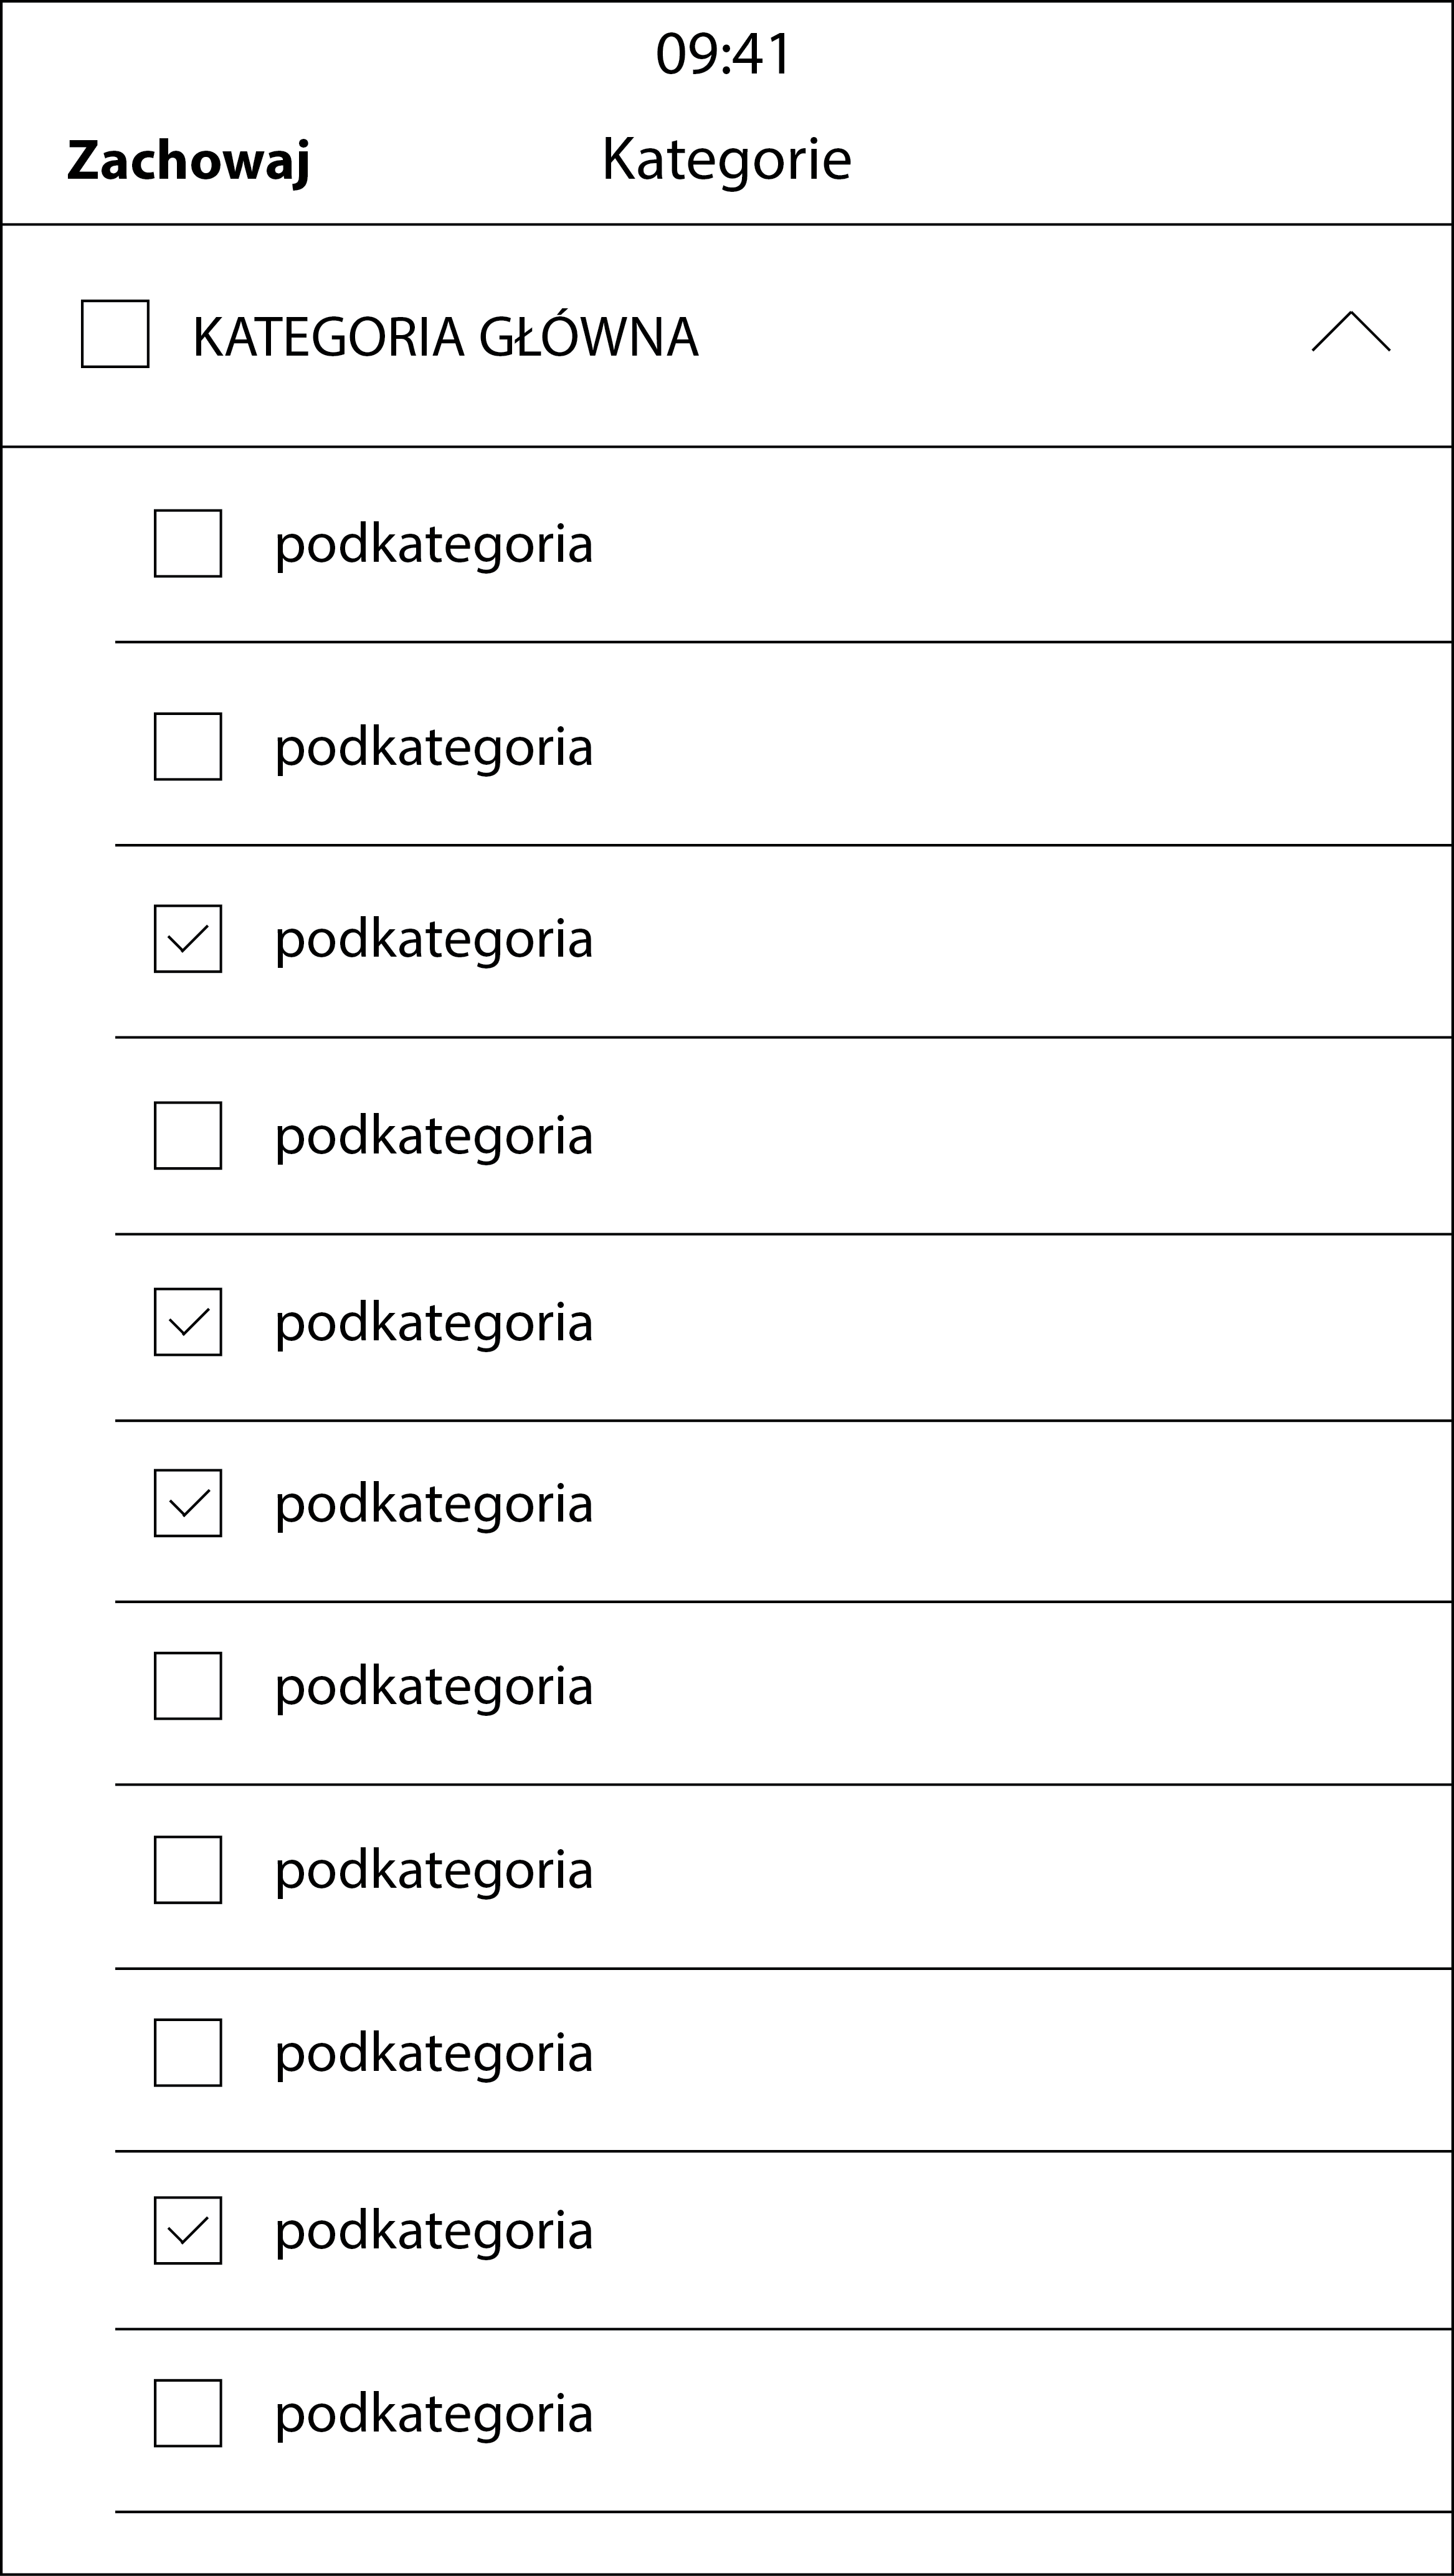
\includegraphics[width=0.4\linewidth]{img/CategoriesProject.png}
  \caption{Projekt ekranu wyboru kategorii}
  \label{fig:androidCategories}
\end{figure}

Aktywność służąca do wyboru kategorii składa się z obiektu \verb`Toolbar` oraz obiektu \verb`ExpandableListView`. Elementami są widoki składające się z obiektów \verb`CheckBox` oraz \verb`TextView` z nazwą kategorii, podobne do elementów widocznych na rysunku \ref{fig:androidCategories}. Podobnie jak poprzednio, w Toolbarze znajduje się nazwa aktualnego widoku, po prawej stronie ikona do usuwania wszystkich do tej pory zaznaczonych elementów, po lewej stronie strzałka powrotu do poprzedniego widoku. 

Podczas powrotu do poprzedniej aktywności, zaznaczone elementy są przekazane w obiekcie \verb`Intent`. 

\begin{verbatim}
@Override
public void onBackPressed() {
    Intent intent = new Intent();
    intent.putParcelableArrayListExtra(ON_BACK_CATEGORIES_EXTRA, categories);
    setResult(RESULT_OK, intent);
    finish();
}
\end{verbatim} 

Jest to możliwe dzięki implementacji przez obiekt \verb`Category` interfejsu \verb`Parcelable`. Aby instancja obiektu mogła zostać zapisana i przechowana w obiekcie \verb`Parcel` konieczne jest stworzenie statycznej zmiennej \verb`CREATOR`.

\begin{verbatim}

public class Category implements Parcelable {

...

	public static final Creator<Category> CREATOR = new Creator<Category>() {
        @Override
        public Category createFromParcel(Parcel in) {
            return new Category(in);
        }

        @Override
        public Category[] newArray(int size) {
            return new Category[size];
        }
    };

    protected Category(Parcel in) {
        categoryId = in.readString();
        name = in.readString();
        isChecked = in.readByte() != 0;
        isExpanded = in.readByte() != 0;
        subcategories = in.createTypedArrayList(Category.CREATOR);
    }

... 
    
    @Override
    public void writeToParcel(Parcel parcel, int i) {
        parcel.writeString(categoryId);
        parcel.writeString(name);
        parcel.writeByte((byte) (isChecked ? 1 : 0));
        parcel.writeByte((byte) (isExpanded ? 1 : 0));
        parcel.writeTypedList(subcategories);
    }
}
\end{verbatim}


\subsubsection{BookActivity}

\begin{figure}[h]
  \centering
  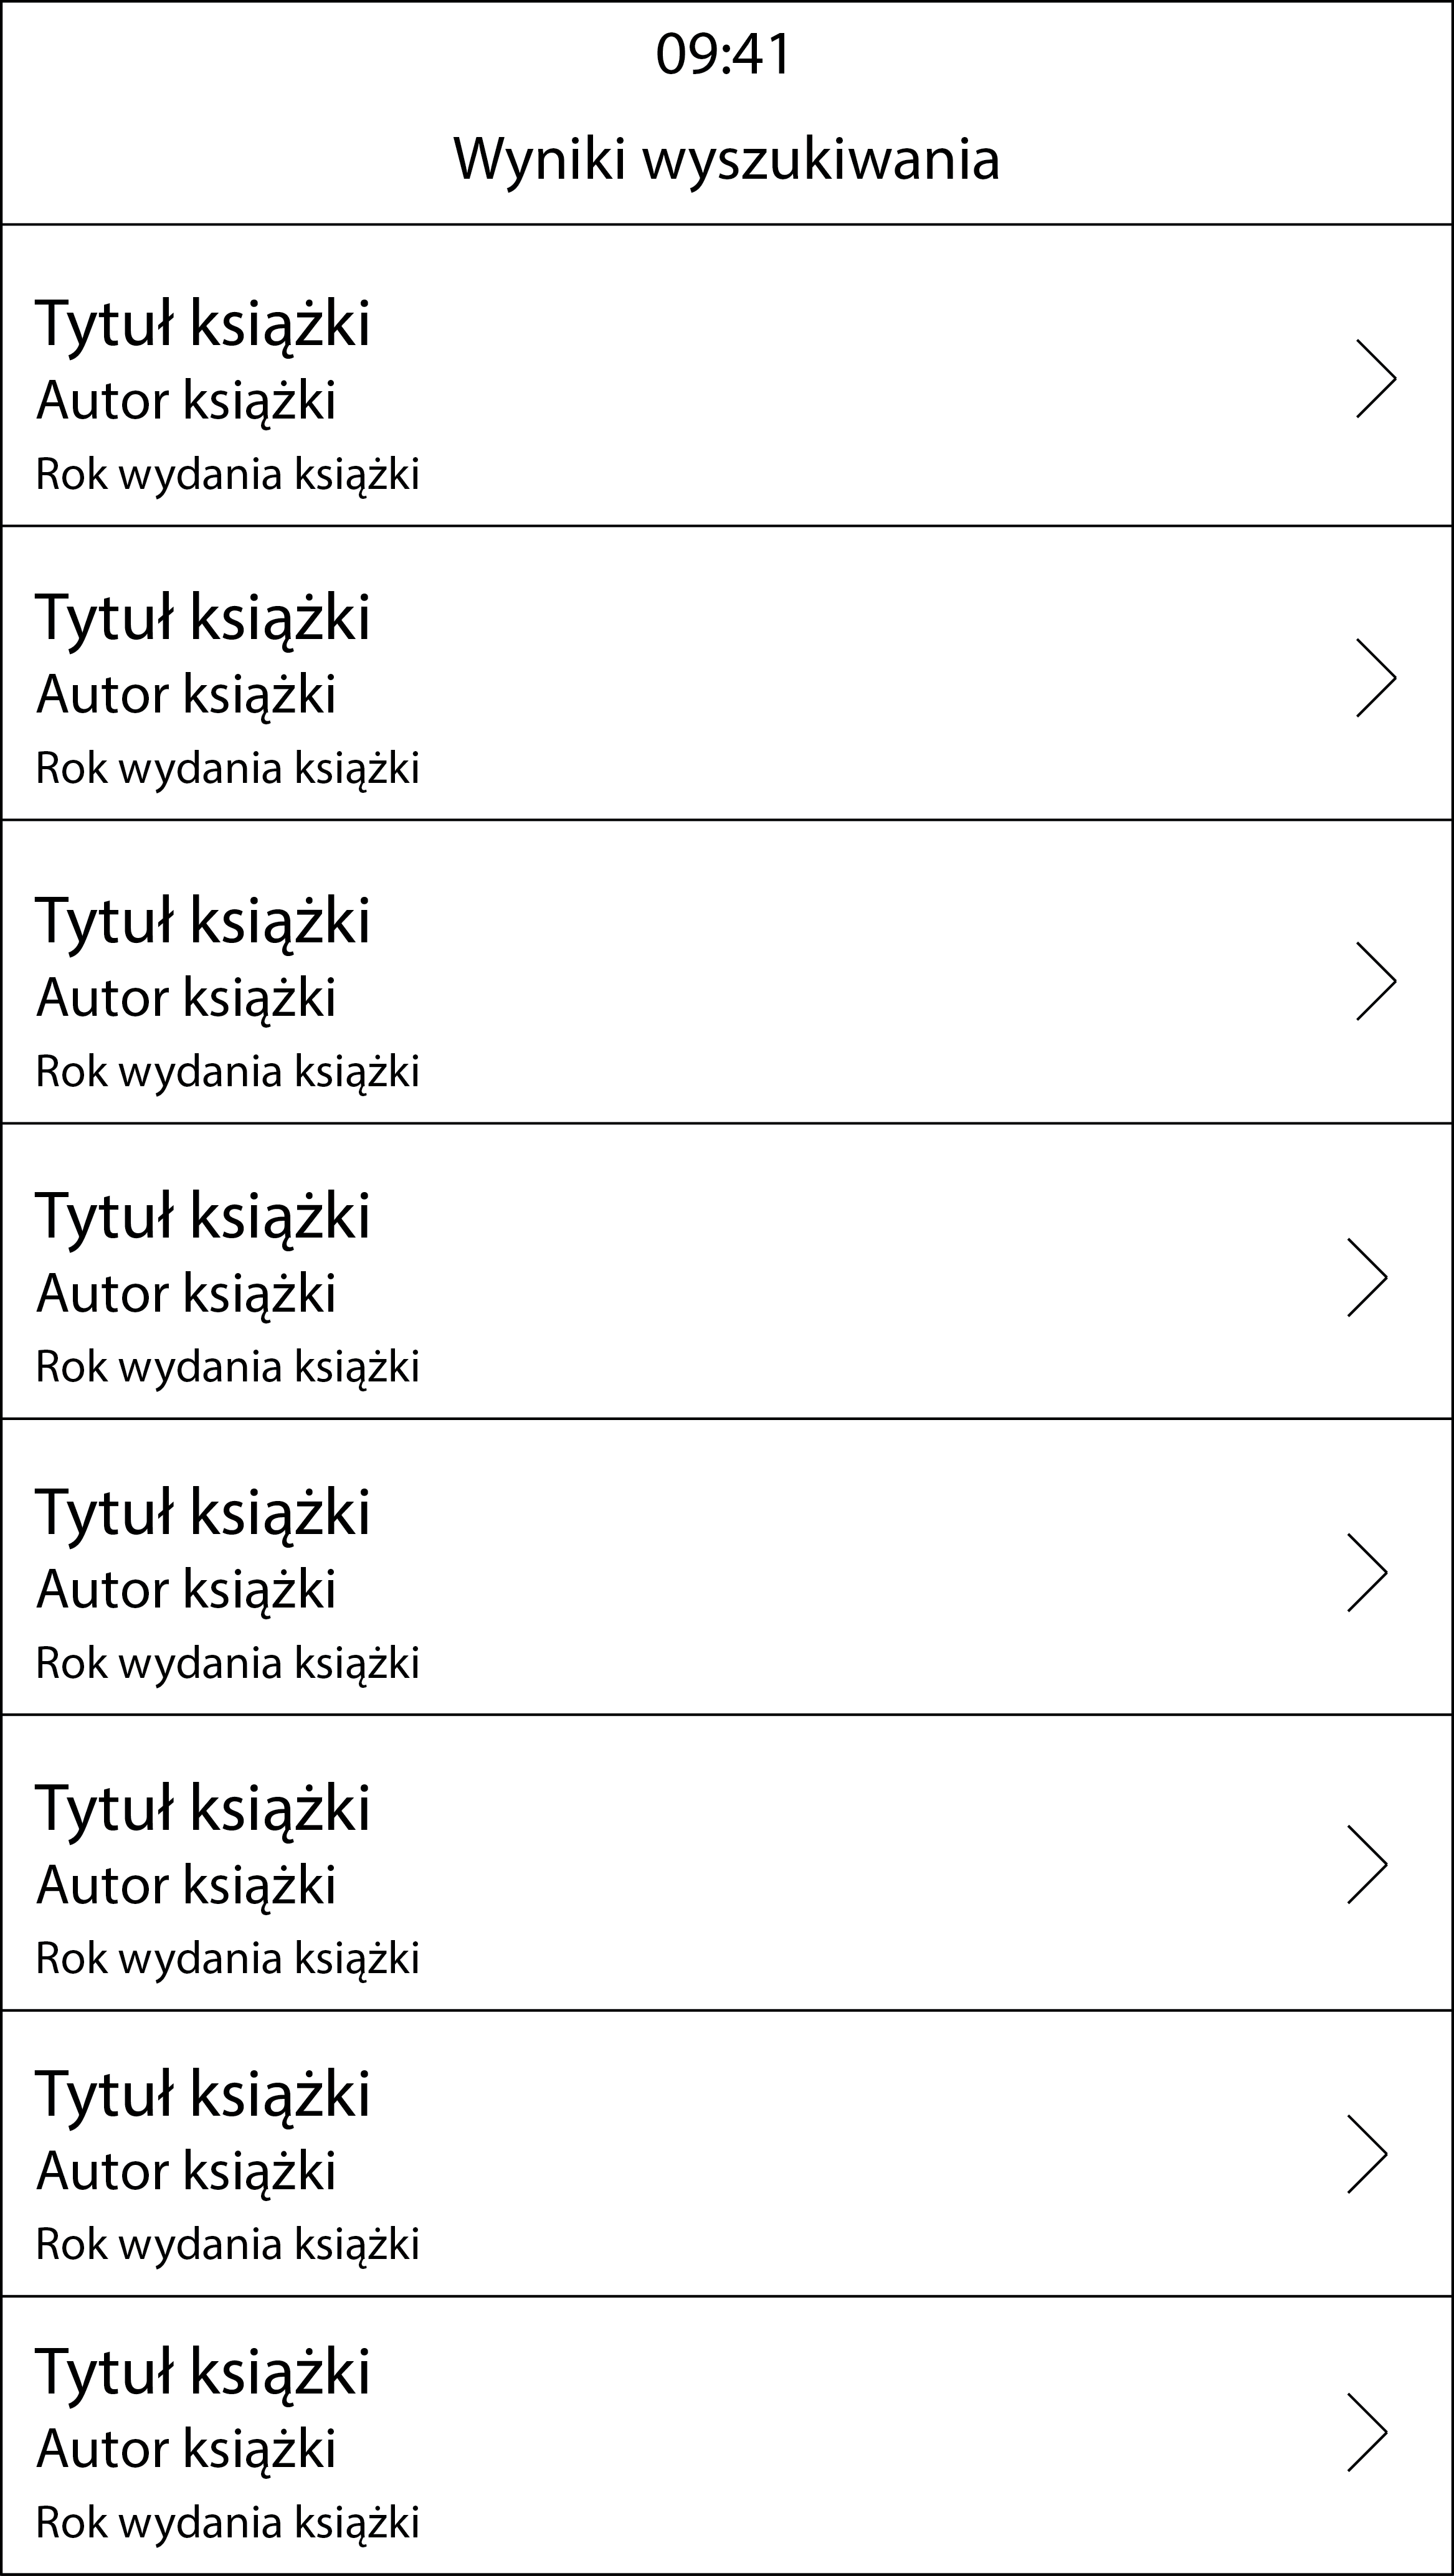
\includegraphics[width=0.4\linewidth]{img/BookListProject.png}
  \caption{Projekt ekranu listy książek}
  \label{fig:bookListAndroid}
\end{figure}

Celem \verb`BookActivity` jest wyświetlenie wszystkich książek, zwróconych przez API. Został użyty do tego element \verb`RecyclerView`. Pozwala on przedstawić dużą liczbę danych na ograniczonym ekranie, podobnie jak na rysunku \ref{fig:bookListAndroid}. Zarządzanie poszczególnymi elementami odbywa się przy użyciu adaptera. W adapterze zapamiętane są wszystkie elementy, w tym przypadki lista książek \verb`List<Book>`. Dla każdej z nich tworzony jest osobny widok z użyciem nadrzędnego szablonu zapamiętanego w \verb`ViewHolderze`. W adapterze do poszczególnych pól, jak na przykład \verb`TextView titleTv` zostaje przypisany tytuł konkretnej książki. Dzięki zapamiętywaniu dwóch pozycji elementu -- pozycja elementu w liście wszystkich obiektów, pozycja elementu z perspektywy \verb`LayoutManagera` -- możliwe jest dynamiczne odświeżanie całego widoku w przypadku jakichkolwiek zmian w danych. 

W aplikacji API dostarcza ograniczoną ilość książek. W przypadku powolnego internetu lub urządzenia nie ma sensu czekać aż serwer zwróci wszystkie możliwe wyniki, a następnie czekać aż aplikacji je przetworzy i wyświetli. Stąd na początku zostaje pobrane np. pierwszych 50 książek. Po doscrollowaniu listy do końca przez użytkownika pobieranych jest kolejnych 50 książek, przy czym poprzednie wyniki są nadal wyświetlane. 

\begin{verbatim}
bookRv.addOnScrollListener(getOnScrollListener());

...

private RecyclerView.OnScrollListener getOnScrollListener() {
    return new RecyclerView.OnScrollListener() {
        @Override
        public void onScrollStateChanged(RecyclerView recyclerView, 
        int scrollState) {
            LinearLayoutManager manager = (LinearLayoutManager)
                recyclerView.getLayoutManager();
            if (isScrollable(scrollState, manager)) {
                currentPage++;
                setupPagination();
                getPresenter().getBooks(bookRequestData);
            }
        }

        private boolean isScrollable(int scrollState, 
            LinearLayoutManager layoutManager) {
            return isEndOfScrollView(layoutManager) 
            && scrollState == SCROLL_STATE_IDLE;
		}

        private boolean isEndOfScrollView(LinearLayoutManager layoutManager) {
            return layoutManager.findLastVisibleItemPosition() 
            == layoutManager.getItemCount() - 1;
        }
    };
}

@Override
public void refreshBooks(List<Book> books) {
    allBooks.addAll(books);
    if (bookRv.getAdapter() != null) {
        bookRv.getAdapter().notifyDataSetChanged();
    }
}
\end{verbatim}

Metoda \verb`isEndOfScrollView(LinearLayoutManager layoutManager)` wykorzystuje pozycję ostatniego widocznego elementu i porównuje ją z pozycją ostatniego elementu w całej liście. Jeśli znajdujemy się na końcu listy zostanie wysłane zapytanie do API o kolejną porcję książek. Po odebraniu odpowiedzi lista z wszystkimi (do tej pory) książkami zostaje zwiększona o nowe książki, a widok odświeżony przez wywołanie metody \verb`notifyDataSetChanged()` na adapterze \verb`RecyclerView`. 

W tej aktywności \verb`Toolbar` zawiera nazwę aktualnego widoku oraz po lewej stronie ikonę powrotu do widoku wyszukiwania książek. 

\subsubsection{BookDetailsActivity}

\begin{figure}[h]
  \centering
  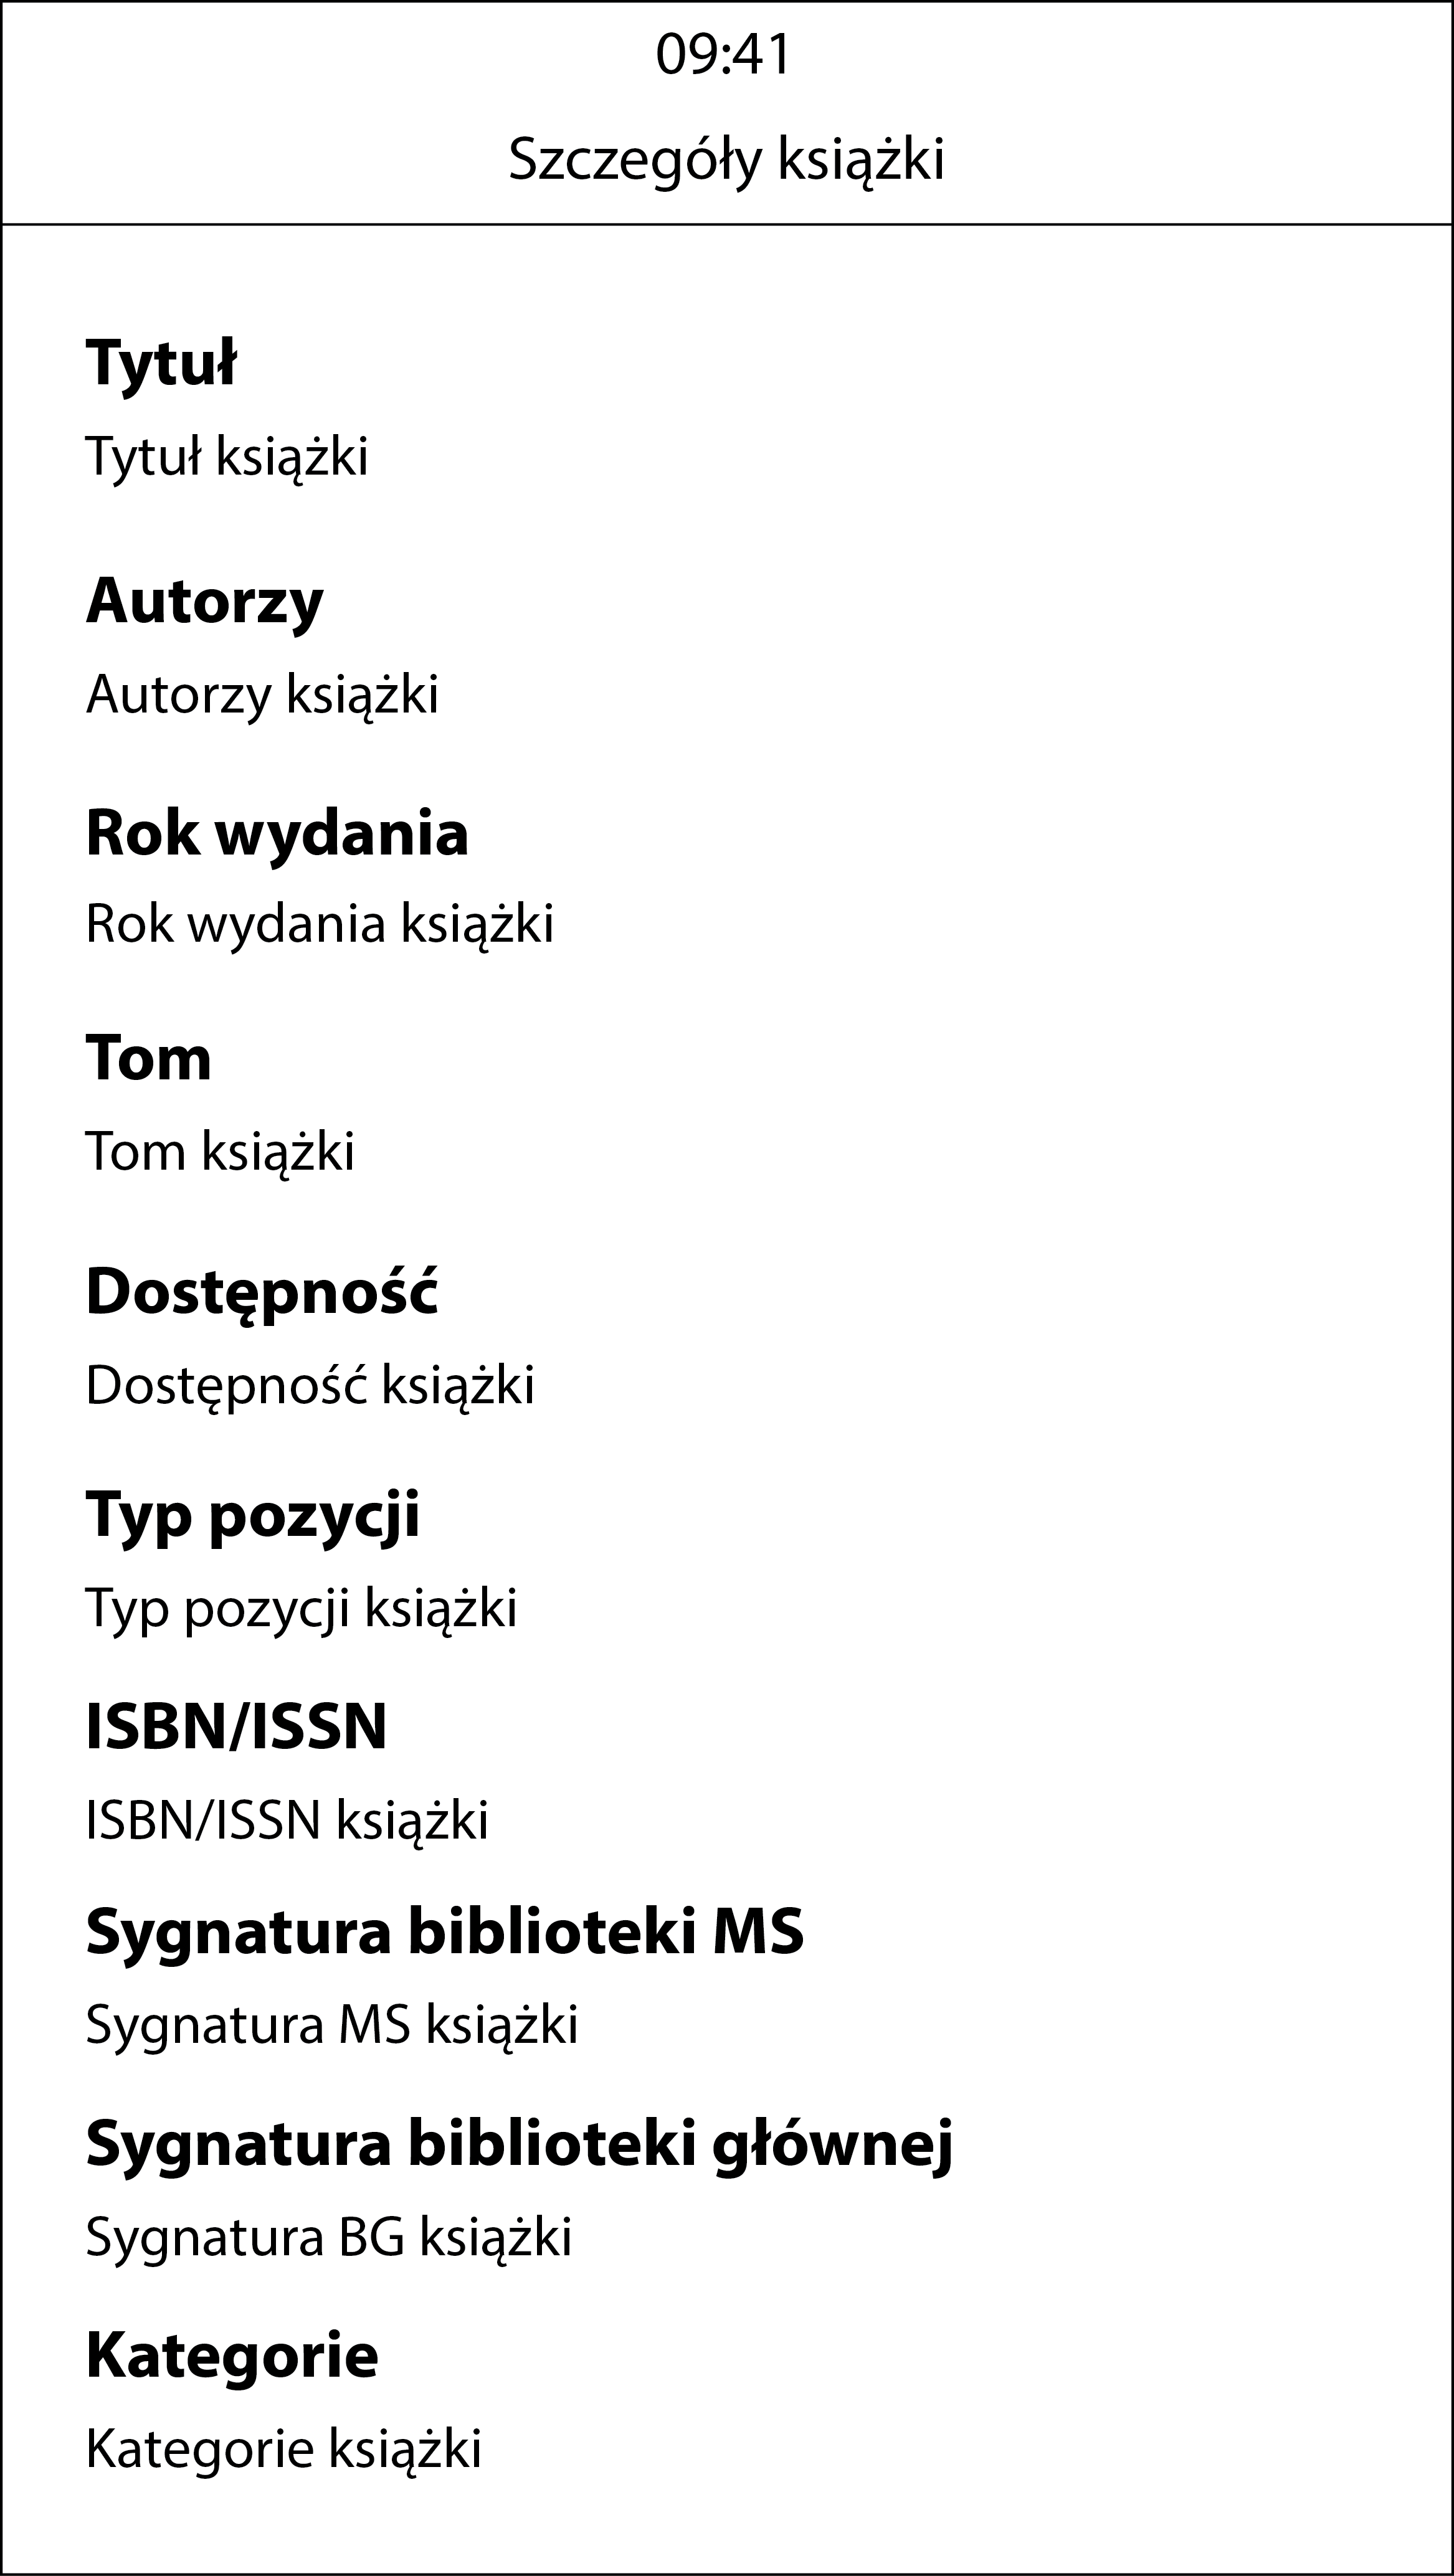
\includegraphics[width=0.4\linewidth]{img/DetailsProject.png}
  \caption{Projekt ekranu szczegółów książki}
  \label{fig:androidDetails}
\end{figure}

Ostatnia aktywność zawiera w sobie szczegółowe informacje o książce (rys. \ref{fig:androidDetails}). Można do niej przejść przez kliknięciu w element na liście wszystkich wyników. Tak jak poprzednie widoki zawiera \verb`Toolbar` z nazwą aktualnego widoku oraz z ikoną powrotu do listy znalezionych książek. Informacje o książce wyświetlane są w polach \verb`TextView`.  

\subsection{Interfejs użytkownika}

Głównym celem aplikacji było ułatwienie studentom Wydziału Matematyki Stosowanej korzystania z biblioteki. W związku z tym powstała aplikacja na jeden z~największych systemów -- Android. Jednocześnie celem aplikacji była jak największa przejrzystość i intuicyjność, aby osoby nie korzystające na co dzień z dotykowych telefonów, również mogły używać jej bez problemów. Projekt był konsultowany na bieżąco z osobą zarządzającą biblioteką. Jednolity \verb`Toolbar` pozwala na łatwą nawigację po aplikacji, a dobór odpowiednich kolorów zagwarantował spójność z aplikacją tworzoną na system iOS.
 
\subsection{Splash screen}

Aplikacja po uruchomieniu wyświetla ekran powitalny (rys. \ref{fig:splashScreen}). 

\begin{figure}[h]
  \centering
  
\includegraphics[width=0.4\linewidth]{img/android/android1.png}
  \caption{Ekran startowy aplikacji}
  \label{fig:splashScreen}
\end{figure}

Ekran po $1.5$ sekundy znika i nie jest możliwe wrócenie do niego po naciśnięciu przycisku \textit{back}.

\subsubsection{Wyszukiwarka książek}

\begin{figure}[h]
  \centering
  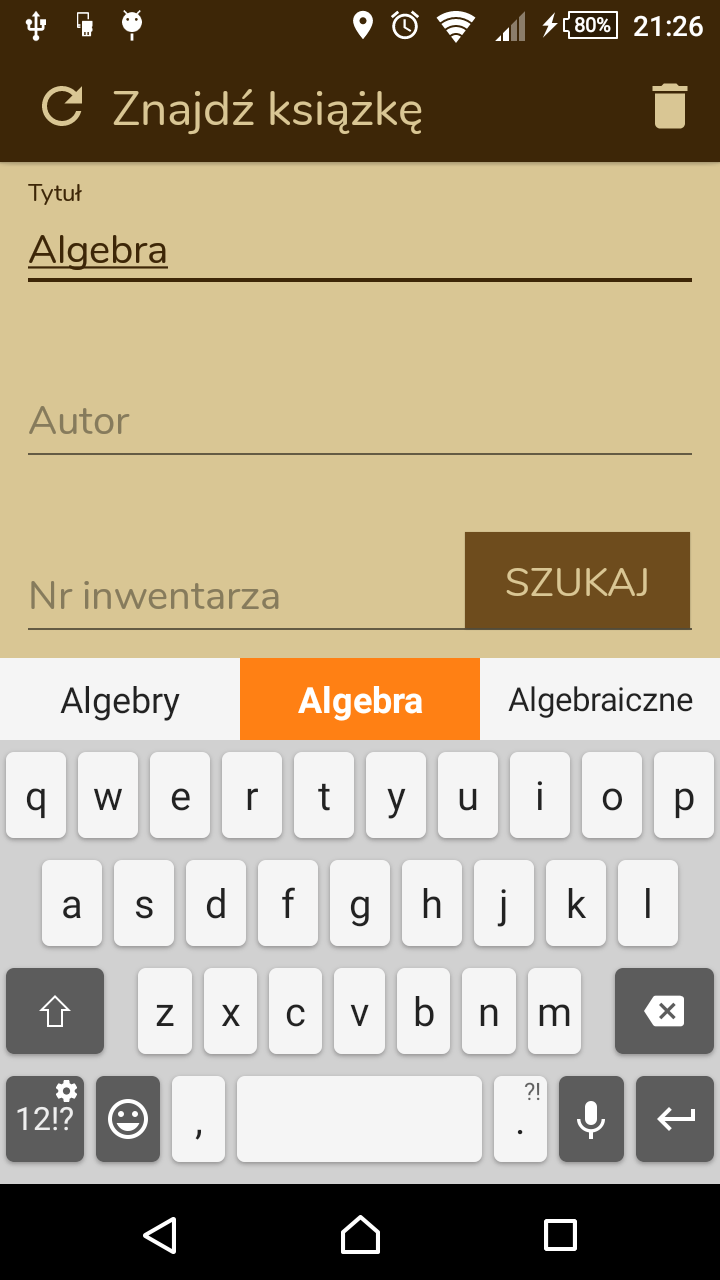
\includegraphics[width=0.4\linewidth]{img/android/android2.png}
  \caption{Wyszukiwarka książek}
  \label{fig:searchScreen}
\end{figure}

Ekran wyszukiwania książek umożliwia użytkownikowi między innymi wpisanie żądanej treści w odpowiednie pola za pomocą klawiatury systemowej (rys. \ref{fig:searchScreen}). Trzy pola znajdujące się najniżej umożliwiają wybranie pozycji z listy. Dwa pierwsze otwierają dialog (rys. \ref{fig:androidSearch2}), ostatnie przenosi do nowej aktywności z listą kategorii, jak na rysunku \ref{fig:androidCategoriesScreen}.

\begin{figure}
    \centering
    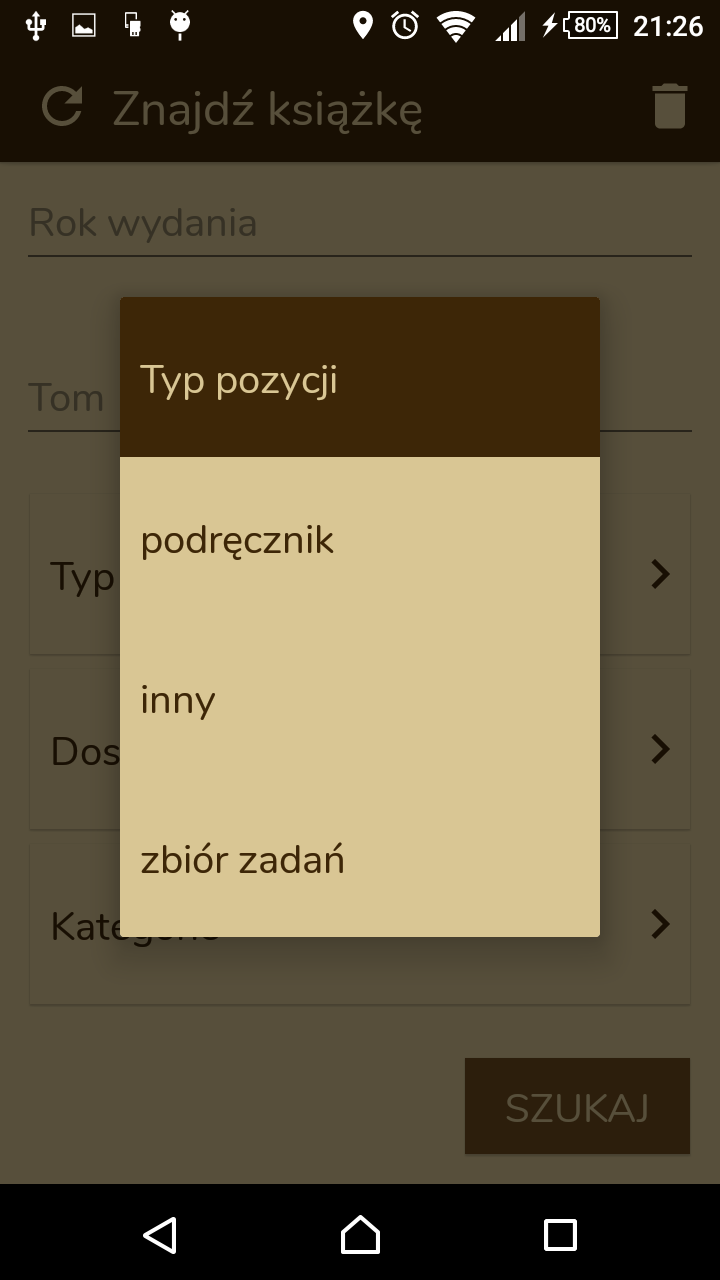
\includegraphics[width=0.4\linewidth]{img/android/android3.png}
    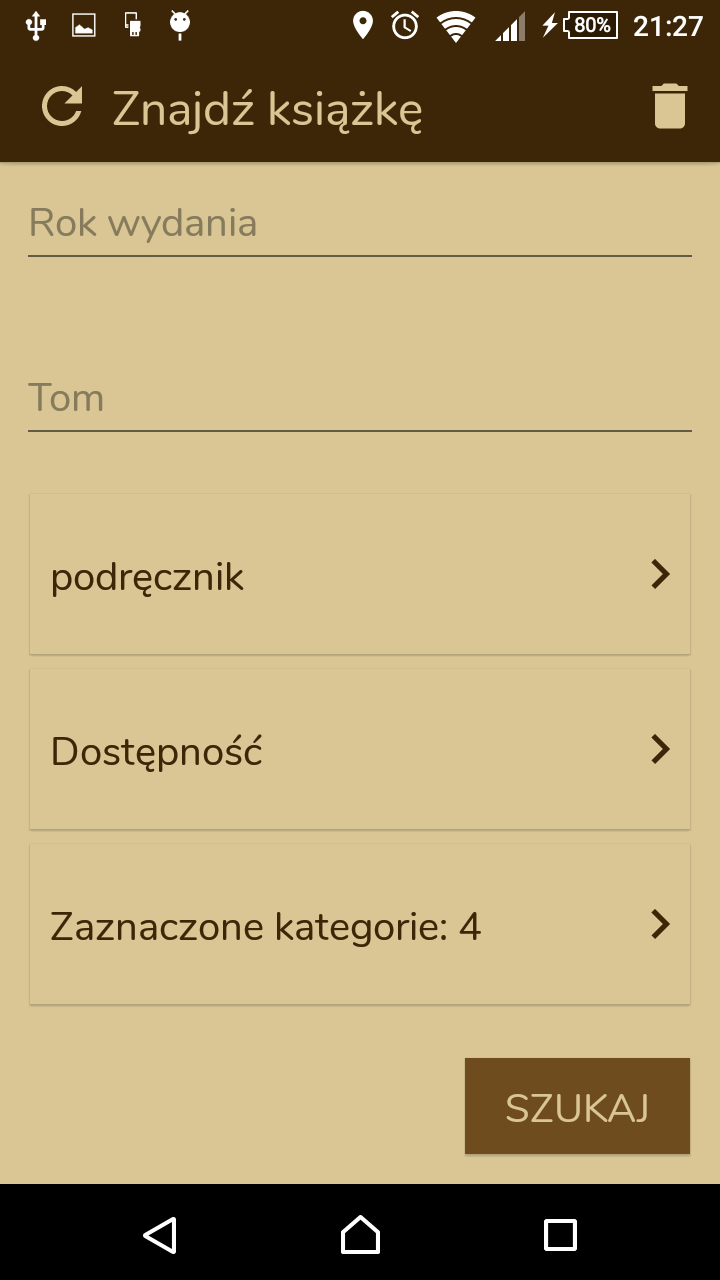
\includegraphics[width=0.4\linewidth]{img/android/android5.png}
    \caption{Dialog z wyborem \textit{typu pozycji} książki oraz widok wyszukiwania po wybraniu typu \textit{podręcznik} przez użytkownika}
    \label{fig:androidSearch2}
\end{figure}

Do poprawnego pobrania danych oraz wyszukania książek aplikacja wymaga połączenia z internetem. W przypadku, gdy nie ma połączenia z internetem, na ekranie pojawi się dialog z informacją o tym oraz \textit{Toast} z informacją o nieudanym pobraniu danych. Przycisk w lewym górnym roku pozwala na odświeżenie danych po uzyskaniu dostępu do internetu.

W dolnym prawym rogu ekranu znajduje się przycisk wyszukiwania. Kliknięcie go otwiera kolejną aktywność i wyszukuje książki.

\subsubsection{Wybór kategorii}

Widok z kategoriami zawiera listę posortowanych elementów podzielonych na sekcję. Można rozróżnić kategorie główne oraz podkategorie, przy czym nie każda kategoria główna zawiera jakieś podkategorie. Jest to oznaczone strzałką znajdującą się z prawej strony elementu, która sugeruje możliwość kliknięcia i rozwinięcia listy. 

Na tym etapie użytkownik ma możliwość ograniczenia zakresu poszukiwanych przez niego książek. Może zaznaczyć dowolną ilość kategorii głównych oraz podkategorii z możliwością szybkiego zresetowania zaznaczonych elementów po naciśnięciu ikony kosza w prawym górnym rogu. 

\begin{figure}[h]
  \centering
  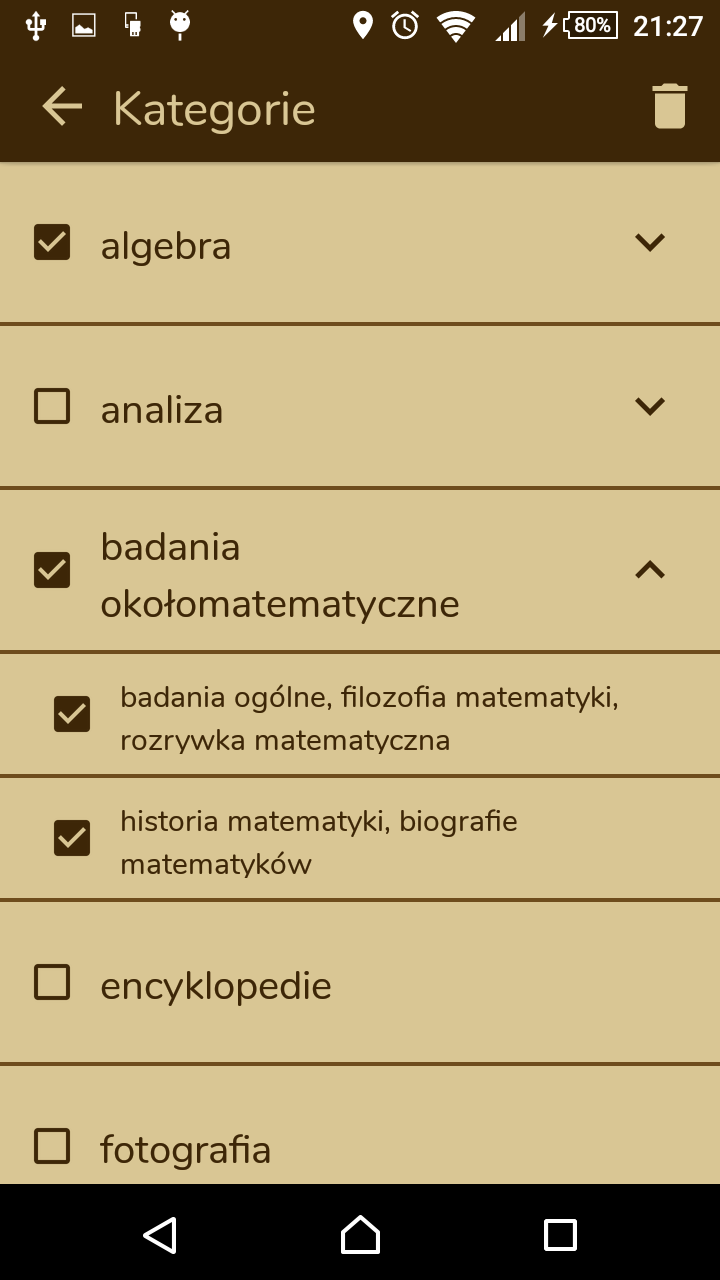
\includegraphics[width=0.4\linewidth]{img/android/android4.png}
  \caption{Ekran wyboru kategorii}
  \label{fig:androidCategoriesScreen}
\end{figure}

W lewym górnym rogu znajduje się strzałka powrotu do poprzedniego widoku. Kliknięcie jej przenosi użytkownika z powrotem na ekran wyszukiwania. Po przeniesieniu na guziku wyboru kategorii pojawia się ilość zaznaczonych przez użytkownika elementów (rys. \ref{fig:androidSearch2}) lub tekst \textit{Kategorie}, w przypadku gdy nic nie zostało zaznaczone.

\subsubsection{Wyniki wyszukiwania}

Po naciśnięciu przez użytkownika przycisku \textit{Szukaj} na ekranie wyszukiwania otworzy się nowy widok. W przypadku nie znalezienia żadnej pozycji pasującej do zapytania lub w przypadku błędu serwera, wyświetlony zostanie ekran znajdujący się na rysunku \ref{fig:androidResults} po prawej stronie. Ekran po lewej z rysunku \ref{fig:androidResults}, przedstawia listę z poprawnie znalezionymi pozycjami. Na tym etapie użytkownik może sprawdzić część tytułu książki (wyświetlanie zależne od wielkości ekranu urządzenia), autora oraz rok wydania. Sortowanie odbywa się alfabetycznie pod względem tytułu. W~przypadku takich samych tytułów sortowanie odbywa się po dacie wydania -- od najnowszej do najstarszej. 

\begin{figure}
\centering
    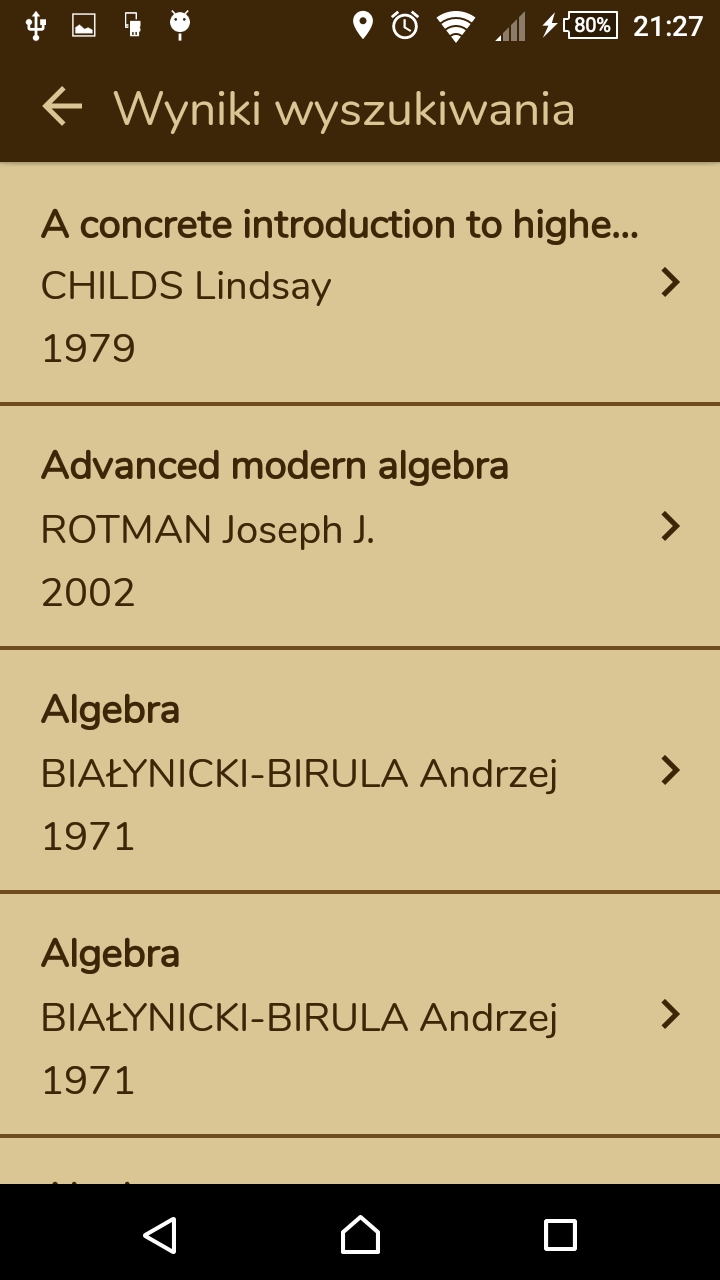
\includegraphics[width=0.4\linewidth]{img/android/android7.png}
    
\includegraphics[width=0.4\linewidth]{img/android/android6.png}
    \caption{Przykładowe wyniki wyszukiwania}
    \label{fig:androidResults}
\end{figure}

Jeśli użytkownik chce wrócić do ekranu wyszukiwania książki może nacisnąć na strzałkę w lewym górnym rogu lub nacisnąć klawisz systemowy znajdujący się w~lewym dolnym rogu na urządzeniach z systemem Android. Po powrocie pola będą wypełnione ostatnio wpisanymi lub wybranymi informacjami.

Więcej szczegółów książki zostanie wyświetlonych po naciśnięciu na konkretną pozycję z listy. 

\subsubsection{Szczegóły książki}

Ekran szczegółów książki został przedstawiony na rysunku \ref{fig:anroidBookDetails}. Tym razem wszystkie znane informacje wyświetlane są w całości. Jeśli elementów jest dużo i nie mieszczą się na ekranie, użytkownik może scrollować widok w celu wyświetlenia pozostałych informacji.

\begin{figure}[h]
  \centering
  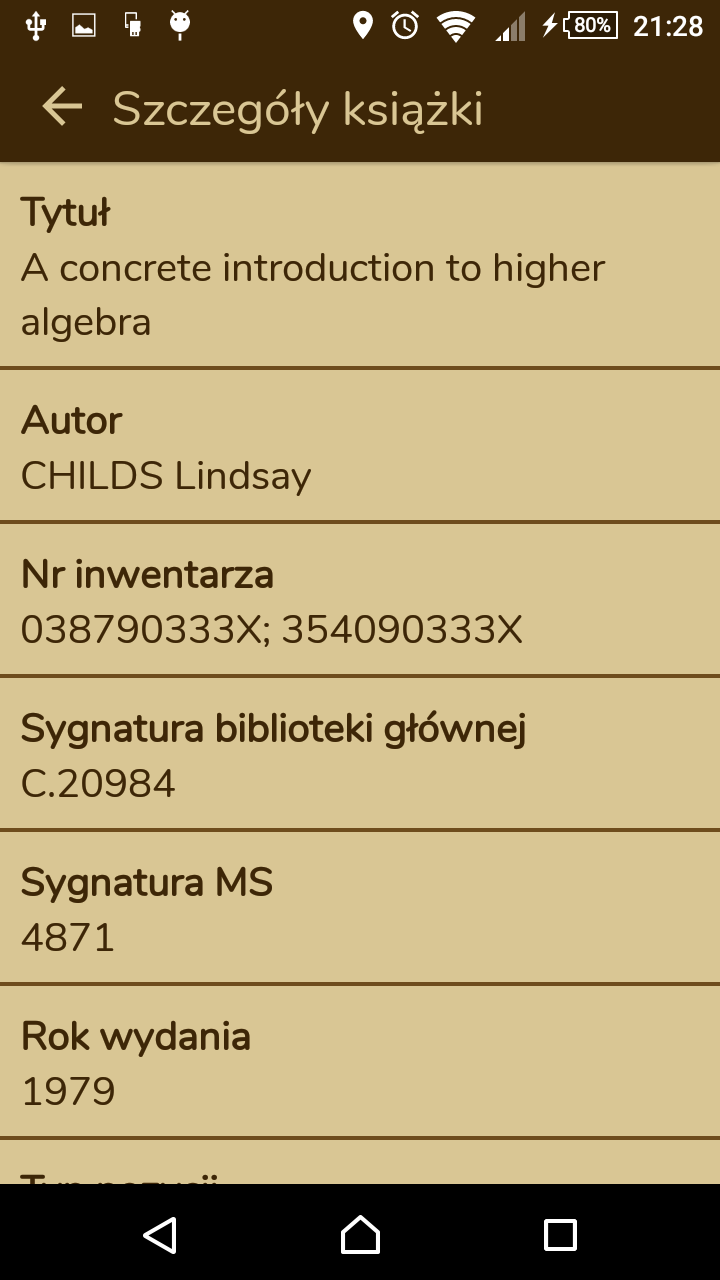
\includegraphics[width=0.4\linewidth]{img/android/android8.png}
  \caption{Szczegóły książki}
  \label{fig:anroidBookDetails}
\end{figure}



\section{Aplikacja na system iOS}

\subsection{Wykorzystane narzędzia}

Aplikacja na system mobilny firmy Apple została napisana w języku \textit{Swift 4}, przy pomocy środowiska \textit{Xcode 9.1}. \textit{Swift} jako język programowania jest dostępny na rynku informatycznym niecałe 4 lata i jest następcą dosyć skomplikowanego języka \textit{Objective--C}. Jego najnowsza, czwarta wersja, która została wykorzystana w~projekcie, miała premierę we wrześniu 2017 roku, w tym samym czasie co dziewiąta wersja środowiska programistycznego \textit{Xcode}. Zatem do tworzenia projektu zostały użyte jedne z najnowocześniejszych narzędzi programistycznych na rynku. Warto dodać, że wykorzystane rozwiązania pozwalają na komercjalizację projektu, ponieważ narzędzie \textit{Xcode} jest programem typu \textit{Freeware}, natomiast język \textit{Swift} bazuje na licencji \textit{Apache License 2.0}, która zezwala na dystrybuowanie i sprzedaż oprogramowania.

\subsection{Wymagania systemowe}

Aplikacja może zostać zainstalowana na systemach iOS w wersji 10.0 lub nowszej. Wybór minimalnej wersji systemu nie był przypadkowy. System ten posiada zalety dla użytkownika jak i dla osoby tworzącej oprogramowanie.

System iOS 10.0 jest systemem istniejącym na rynku od września 2016 roku. Ma on zatem mniej niż półtora roku. Wspieranie tak nowych systemów wydaje się mało sensowne, jednak jest zupełnie inaczej. W przypadku polityki firmy Apple, systemy iOS wspierają zwykle wiele urządzeń istniejących na rynku dużo wcześniej od oficjalnej premiery systemu. Przykładowo wspierając system iOS 10.0, wspieramy zarazem telefon iPhone 5, który to miał premierę we wrześniu 2012. Zatem aplikacja może być instalowana na telefonach sprzed niemal 5.5 roku. Wpływa to zwykle na dużą liczbę instalacji nowych wersji iOS na urządzeniach. Zgodnie ze statystykami \cite{iosStatistics} na dzień 18 stycznia 2018 roku, ilość urządzeń posiadających system iOS wygląda następująco w zależności od wersji:
\begin{itemize}
\item iOS 11 -- $65\%$
\item iOS 10 -- $28\%$
\item wcześniejsze wersje iOS -- $7\%$
\end{itemize}

Z powyższych statystyk wynika, iż pisząc aplikację na system iOS 10.0, można wspierać $93\%$ rynku urządzeń mobilnych z systemem firmy Apple. Dodatkowo wspieranie stosunkowo nowej wersji systemu przynosi także inne korzyści a mianowicie dłuższy okres czasu istnienia na rynku w przypadku rzadkiego aktualizowania aplikacji.

Jeśli chodzi o spojrzenie na zasadność wspierania systemu iOS 10.0 od strony programisty, można z pewnością stwierdzić, że im nowszy system tym więcej narzędzi do zastosowania podczas tworzenia oprogramowania. Nowe wersje systemów zwykle przynoszą łatwiejsze i szybsze rozwiązania, które mogą być wykorzystane. Zatem najwygodniej dla programisty jest wytwarzać produkt stosując coraz to nowocześniejsze metody. Z tego względu wybór wspierania systemu iOS 10.0 jest pewnego rodzaju kompromisem pomiędzy programistą a klientem. Programista zyskuje odpowiednią wygodę podczas tworzenia aplikacji, a klient zyskuje nowoczesny produkt, który przez długi czas może utrzymać się na rynku aplikacji mobilnych.


\subsection{Model danych}
Aplikacja posiada następujący model danych:
\begin{itemize}
\item \verb`Book` -- najważniejsza klasa aplikacji. Reprezentuje obiekt książki. Implementuje protokół \verb`Codable`.
\begin{itemize}
\item \verb`bookTitle` (\verb`String`) -- tytuł
\item \verb`bookAuthors` (\verb`String`) -- autorzy
\item \verb`bookYear` (\verb`String`) -- rok wydania
\item \verb`bookVolume` (\verb`String`) -- tom
\item \verb`bookAvailability` (\verb`String`) -- dostępność
\item \verb`bookPositionType` (\verb`String`) -- typ pozycji
\item \verb`bookIsbn` (\verb`String`) -- numer ISBN
\item \verb`bookMathLibrarySignature` (\verb`String`) -- sygnatura biblioteki MS
\item \verb`bookMainLibrarySignature` (\verb`String`) -- sygnatura biblioteki głównej
\item \verb`bookCategories` (\verb`[Category]`) -- kategorie, do których książka jest przypisana
\end{itemize}
\item \verb`MainCategory` -- klasa reprezentująca kategorię główną. Implementuje protokół \verb`Decodable`.
\begin{itemize}
\item \verb`category` (\verb`Category`) -- kategoria
\item \verb`subcategoriesArray` (\verb`[Category]`) -- tablica podkategorii, przypisanych do kategorii głównej
\end{itemize}
\item \verb`Category` -- klasa reprezentująca obiekt kategorii. Implementuje protokół \verb`Codable`.
\begin{itemize}
\item \verb`id` (\verb`String`) -- id kategorii
\item \verb`name` (\verb`String`) -- nazwa kategorii
\end{itemize}
\item \verb`DictionaryTypes` -- model opisujący obiekt słownika dla książki. Implementuje protokół \verb`Codable`.
\begin{itemize}
\item \verb`type` (\verb`[String]`) -- typy pozycji (np. podręcznik, zbiór zadań, inny)
\item \verb`availability` (\verb`[String]`) -- dostępność (np. dostępna, wypożyczona, czytelnia)
\end{itemize}
\end{itemize}

Analizując powyższy model danych, który został wykorzystany w aplikacji, warto wspomnieć, że można podzielić kategorie na dwa rodzaje: kategorię główną oraz podkategorię. Każdy z tych rodzajów można jednak przedstawić za pomocą obiektu typu \verb`Category`. Zatem pole \verb`categories` może posiadać w tablicy kategorie jak i~kategorie główne. Wystarczy z kategorii głównej wyciągnąć pole \verb`category`.


\subsection{Realizacja projektu}

Projekt był realizowany przy pomocy natywnych narzędzi. Proces tworzenia widoków został oparty o narzędzie \textit{Interface Builder} dostarczane przez firmę Apple. Umożliwia on budowanie widoków za pomocą prostego przenoszenia komponentów i ustawiania odległości pomiędzy nimi z poziomu interfejsu. Pozwala to na szybkie i proste tworzenie widoków aplikacji.

Główne widoki aplikacji zostały utworzone w pliku o nazwie \textit{Main.storyboard}, który pozwala na wykorzystanie opisanego powyżej narzędzia. Wszystkie podrzędne widoki takie jak komórki tabeli, zostały utworzone w plikach o rozszerzeniu \textit{.xib}. Osobny plik dla każdej z komórek pozwala na ich ułatwione modyfikacje w przyszłości oraz wielokrotne używanie w różnych tabelach.

Każdy z utworzonych widoków ma swoje odzwierciedlenie w pliku typu \textit{.swift}. Dzięki temu programista ma możliwość wpływania na ich wygląd zewnętrzny za pomocą przekazywania im odpowiednich danych.

Proces tworzenia aplikacji na system iOS bazował na ciągłych porównaniach aplikacji z aplikacją na system Android w celu jak najlepszego odwzorowania obu z tych aplikacji. Wiele z wykorzystanych rozwiązań było dostępne wyłącznie dla wybranej platformy. Poniżej zostały przedstawione istotne elementy, jakie użyto podczas tworzenia oprogramowania dla biblioteki wydziałowej na mobilny system firmy Apple.


\subsubsection{Biblioteka R.swift}

\textit{R.swift} jest biblioteką \cite{Rswift}, która służy do zarządzania zasobami aplikacji. Została ona wciągnięta do projektu na początku jego tworzenia w celu wygody dostępu do elementów aplikacji. Działa bardzo podobnie do klasy \verb`R` występującej w języku Java dla systemu Android. Dzięki tej bibliotece można w bardzo łatwy sposób dostać się do komponentów takich jak obrazek, zainicjowany widok czy też międzynarodowe ciągi znaków zapisane w aplikacji. Przykładem pokazującym zasadność użycia tej biblioteki może być zwykłe rejestrowanie komórki do tabeli.
\begin{verbatim}
tableView.register(
    UINib(nibName: "BookTableViewCell", bundle: nil),
    forCellReuseIdentifier: "BookTableViewCell"
)
\end{verbatim}
Poniższy przykład pokazuje uproszczony sposób rejestrowania komórki przy pomocy biblioteki \textit{R.swift}.
\begin{verbatim}
tableView.register(
    R.nib.bookTableViewCell(),
    forCellReuseIdentifier: "BookTableViewCell"
)
\end{verbatim}


\subsubsection{Zarządzanie widokami}

Cała aplikacja na system iOS została stworzona z wykorzystaniem natywnego narzędzia jakim jest \verb`UIPageViewController` \cite{AppleDeveloper}. Pozwala on na przechodzenie pomiędzy widokami typu \verb`UIViewController` z wykorzystaniem jednej z dwóch natywnych animacji, które można wybrać. W przypadku naszej aplikacji wykorzystana została animacja \verb`pageCurl`, która imituje przewracanie strony w książce. Pozwoliło to na lepszy odbiór aplikacji przez użytkownika.

Obiekt klasy \verb`UIPageViewController` działa na zasadzie tablicy uporządkowanej widoków, co oznacza, że każdy z widoków ''wie'' jaki widok jest przed nim i~za nim. Nasza aplikacja nie ma ustalonej kolejności widoków, ponieważ użytkownik za każdym razem ma pewien wybór i może przejść do jednego widoku, by potem wrócić i przejść do kolejnego. Z tego powodu, w celu skorzystania z tego narzędzia, została utworzona klasa \verb`MainPageViewController`, która dziedziczy po klasie \verb`UIPageViewController` w celu dostosowania jej do naszych potrzeb. Została ona zaimplementowana w taki sposób, by przed każdym przejściem pomiędzy widokami następowała analiza, jaki widok ma być wyświetlony. Następnie jest on tworzony, uzupełniany odpowiednimi danymi i pokazywany z pewnym wybranym przejściem (w prawo lub w lewo). Dodatkowo obiekt typu \verb`MainPageViewController` ma możliwość zaprezentowania widoku oraz zainicjowania systemowego paska nawigacji. W~celu umożliwienia wykonania tych operacji z dowolnego wyświetlonego widoku, został utworzony odpowiedni protokół, który jest implementowany przez tę klasę, a~następnie wykorzystywany w widokach, które go wymagają do obsługi interfejsu użytkownika.
\begin{verbatim}
protocol MainPageViewControllerDelegate: class {
    func presentViewController(_ viewController: UIViewController)
    func next(viewController: UIViewController)
    func previous(viewController: UIViewController)
    func initNavigationBar(withTitle title: String?,
                           leftButton: UIBarButtonItem?,
   	                       rightButton: UIBarButtonItem?)
}
\end{verbatim}
Każdy z widoków podrzędnych posiada pole typu \verb`MainPageViewControllerDelegate?`, które pozwala na przekazanie metod służących do zarządzania interfejsem bezpośrednio z poziomu tego widoku.


\subsubsection{MainViewController}

Klasa ta dziedziczy po klasie \verb`UIViewController` i została stworzona jedynie w~celu możliwości rozszerzenia funkcjonalności aplikacji w przyszłości. Jest ona bowiem dziedziczona przez każdy widok w aplikacji, co pozwala na zunifikowanie interfejsu poprzez dostęp do tych samych metod, które są w stanie wpłynąć na utworzoną instancję widoku.


\subsubsection{SearchViewController}

\begin{figure}[h]
  \centering
  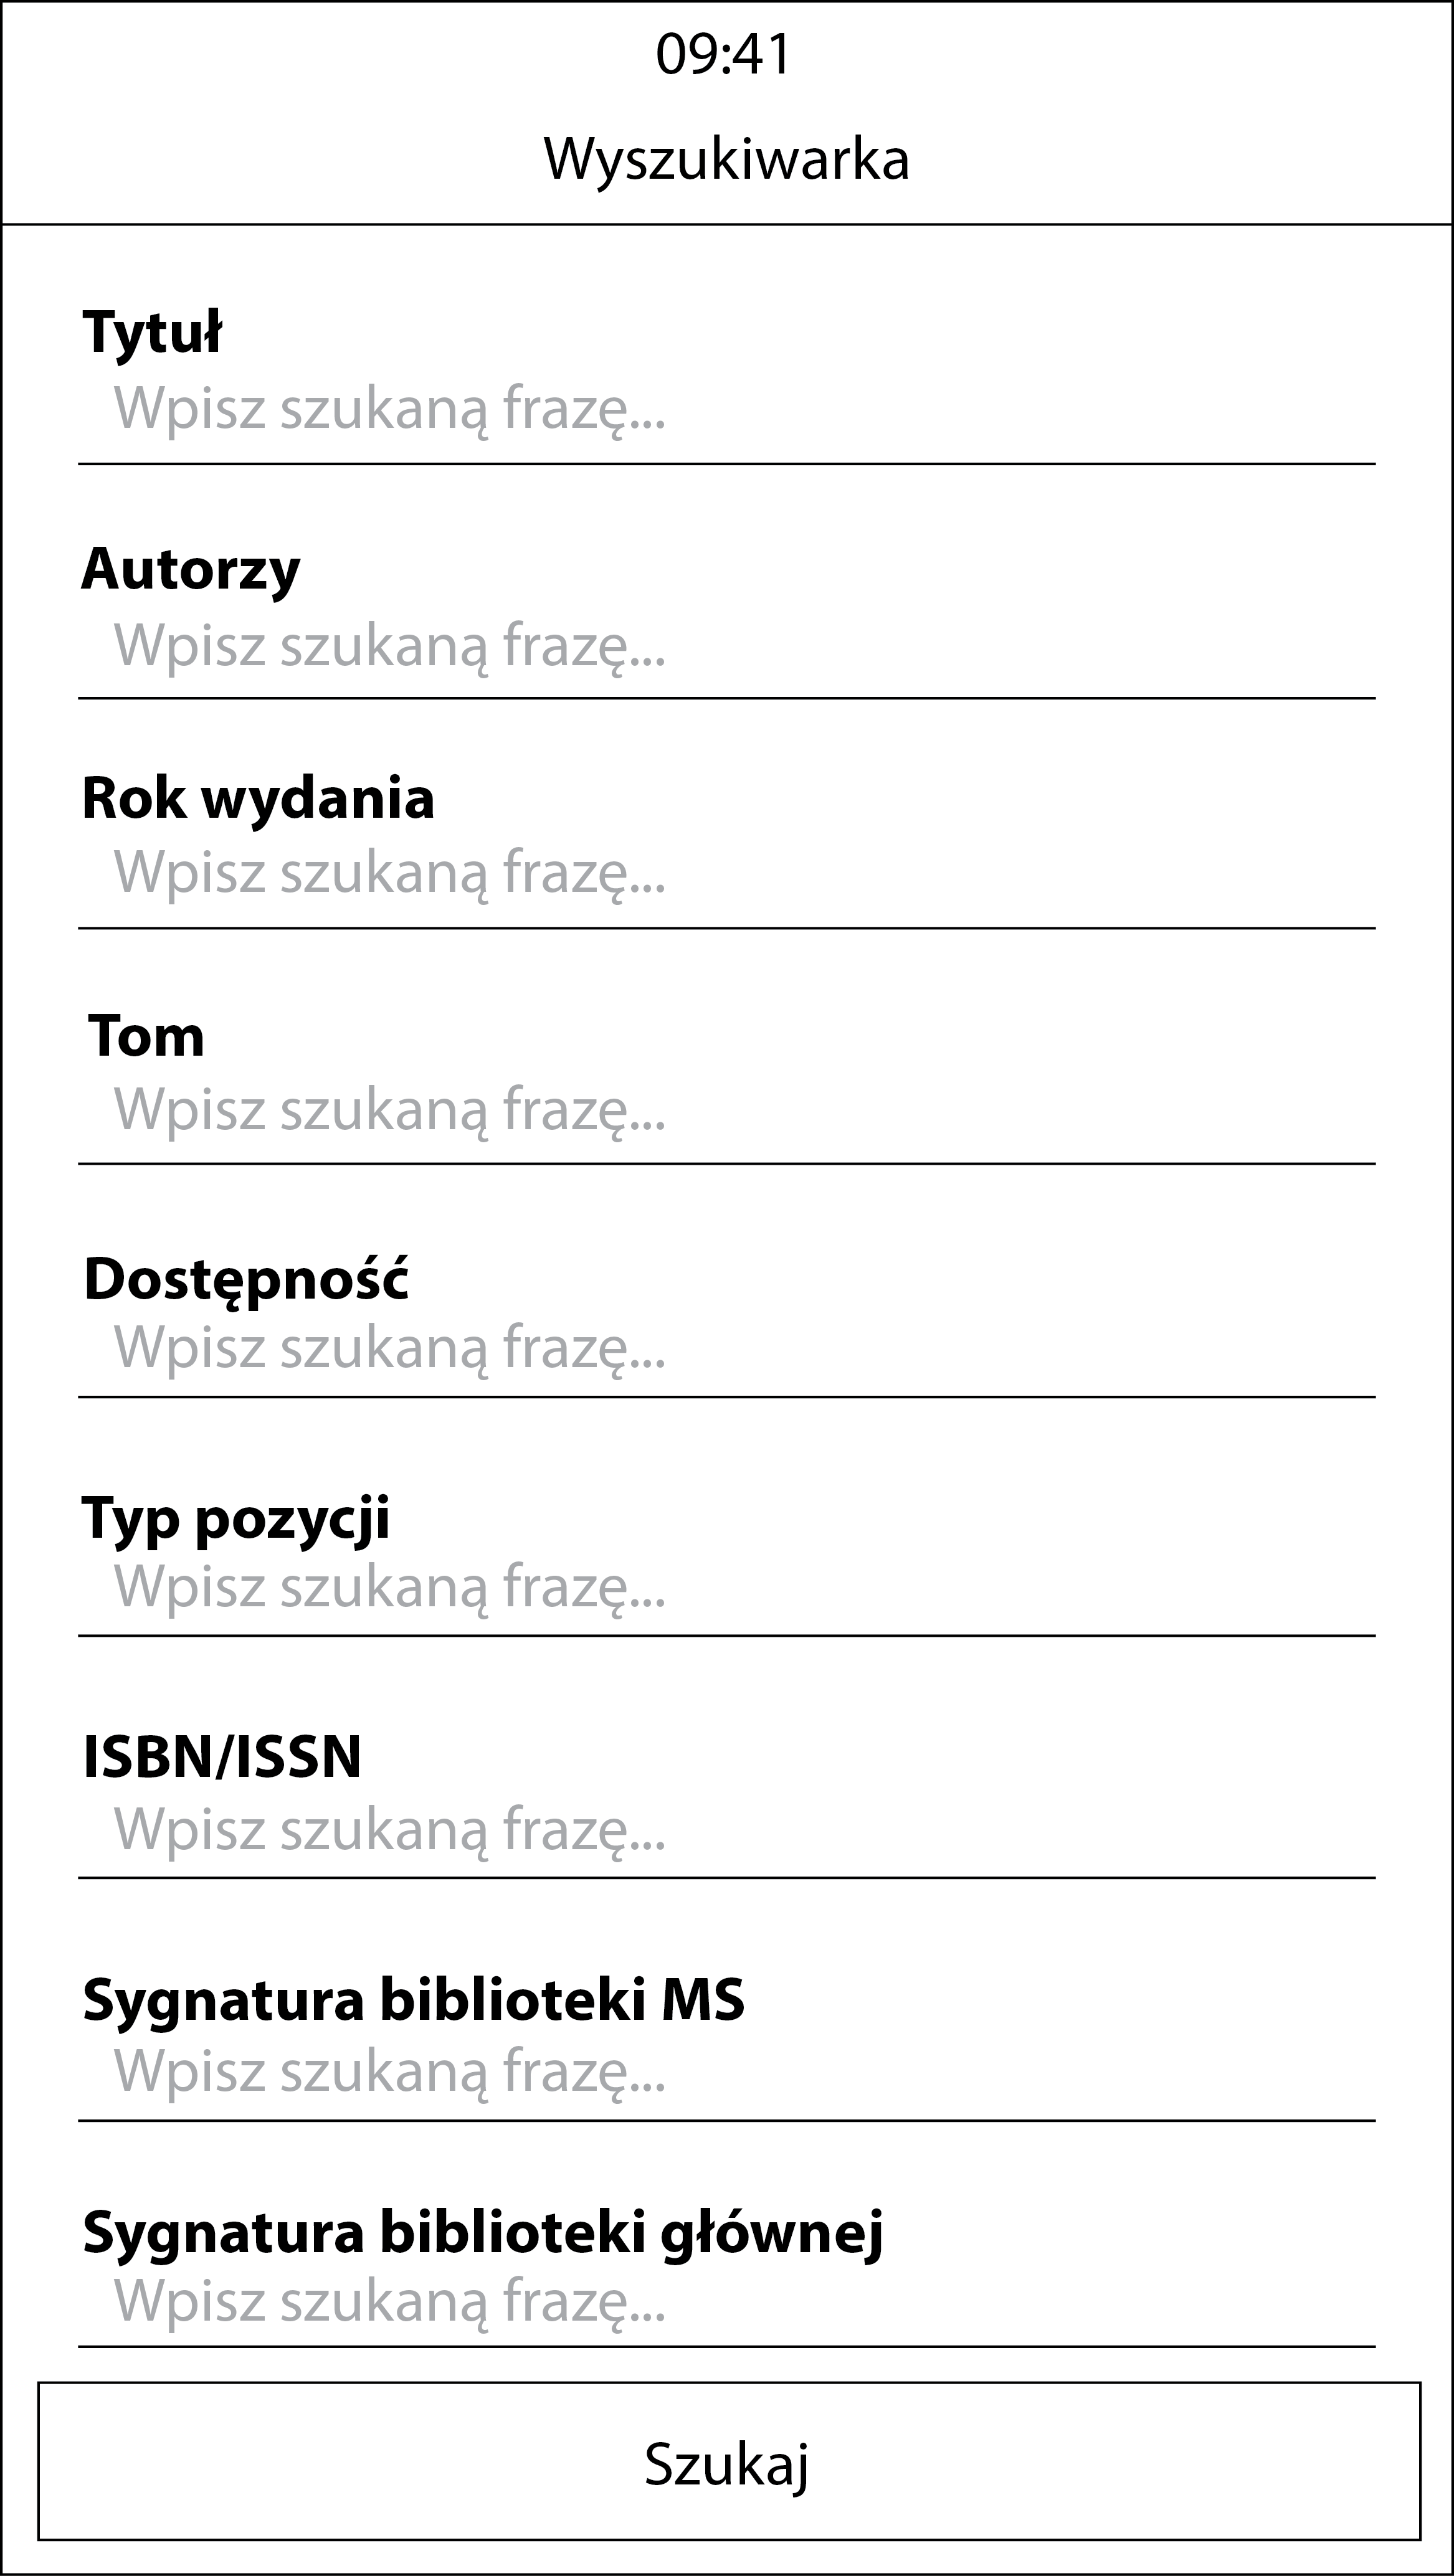
\includegraphics[width=0.4\linewidth]{img/SearchProject.png}
  \caption{Projekt ekranu wyszukiwania książek}
  \label{fig:iosCategories}
\end{figure}

Obiekt klasy tego typu jest obiektem pozwalającym przygotować formularz, który następnie będzie użyty w celu wyszukania książki w systemie biblioteki. Składa się on z natywnego elementu tabeli \verb`UITableView`, dwóch rodzajów komórek: \verb`SearchTextTableViewCell` i \verb`SearchCategoryTableViewCell` oraz z przycisku typu \verb`LoadingButton`, który został zaimplementowany na potrzeby projektu. Klasa \verb`SearchViewController` implementuje delegaty obu tych komórek:
\begin{itemize}
\item \verb`SearchTextTableViewCellDelegate` -- w celu odczytania tekstu z komórki i~zapisania odczytanego ciągu znaków w celu użycia go do wyszukiwania
\item \verb`SearchCategoryTableViewCellDelegate` -- w celu przekazania możliwości otwarcia widoku z kategoriami, po naciśnięciu przycisku 
\end{itemize}

Widok typu \verb`SearchCategoryTableViewCell` posiada możliwość uzupełniania danych przez użytkownika. Powoduje to wysunięcie się klawiatury, która niekiedy zakrywa pole, w które użytkownik wpisuje tekst. Z tego powodu został on wyposażony w rozszerzenie, które pozwala na podwijanie się widoku podczas wysuwania na nim klawiatury.

\begin{verbatim}
extension SearchViewController {
    @objc func keyboardWillShow(notification:NSNotification){
        var userInfo = notification.userInfo!
        var keyboardFrame:CGRect =
        (userInfo[UIKeyboardFrameEndUserInfoKey] as! NSValue)
        .cgRectValue
        keyboardFrame = self.view.convert(keyboardFrame, from: nil)
        tableView.contentInset =
        UIEdgeInsetsMake(0.0, 0.0,
            keyboardFrame.size.height + 8.0, 0.0)
    }
    @objc func keyboardWillHide(notification:NSNotification){
        var userInfo = notification.userInfo!
        var keyboardFrame:CGRect =
        (userInfo[UIKeyboardFrameEndUserInfoKey] as! NSValue)
        .cgRectValue
        keyboardFrame = self.view.convert(keyboardFrame, from: nil)
        tableView.contentInset =
        UIEdgeInsetsMake(0.0, 0.0,
            DefaultValues.EDGE_INSET_BOTTOM, 0.0)
    }
}
\end{verbatim}

Powyższe metody w celu monitorowania zachowania klawiatury są dodane do centrum notyfikacji w aplikacji jako obserwatory pokazania/ukrycia się natywnej klawiatury.

\begin{verbatim}
private func initObservers() {
        NotificationCenter.default.addObserver(self,
            selector: #selector(keyboardWillShow),
            name: NSNotification.Name.UIKeyboardWillShow,
            object: nil)
        NotificationCenter.default.addObserver(self,
            selector: #selector(keyboardWillHide),
            name: NSNotification.Name.UIKeyboardWillHide,
            object: nil)
    }
\end{verbatim}

Widok posiada u dołu przycisk szukania, który odpytuje usługę za pomocą spreparowanego obiektu klasy \verb`Book` utworzonego na podstawie uzupełnionych pól przez użytkownika.

W pasku nawigacji widoku, zostały podpięte dwa przyciski. Jeden z nich znajduje się po lewej stronie i służy do pobrania typów pozycji, dostępności oraz kategorii książek w przypadku braku internetu przy włączaniu aplikacji. Kliknięcie tego przycisku powoduje także wyświetlenie dialogu informującego użytkownika o pobieraniu danych. Do utworzenia dialogu została wykorzystana biblioteka JGProgressHUD \cite{JGProgressHUD}. Drugi z przycisków znajduje się po prawej stronie i służy do wyczyszczenia formularza ze wszystkich wpisanych danych.


\subsubsection{CategoriesViewController}

\begin{figure}[h]
  \centering
  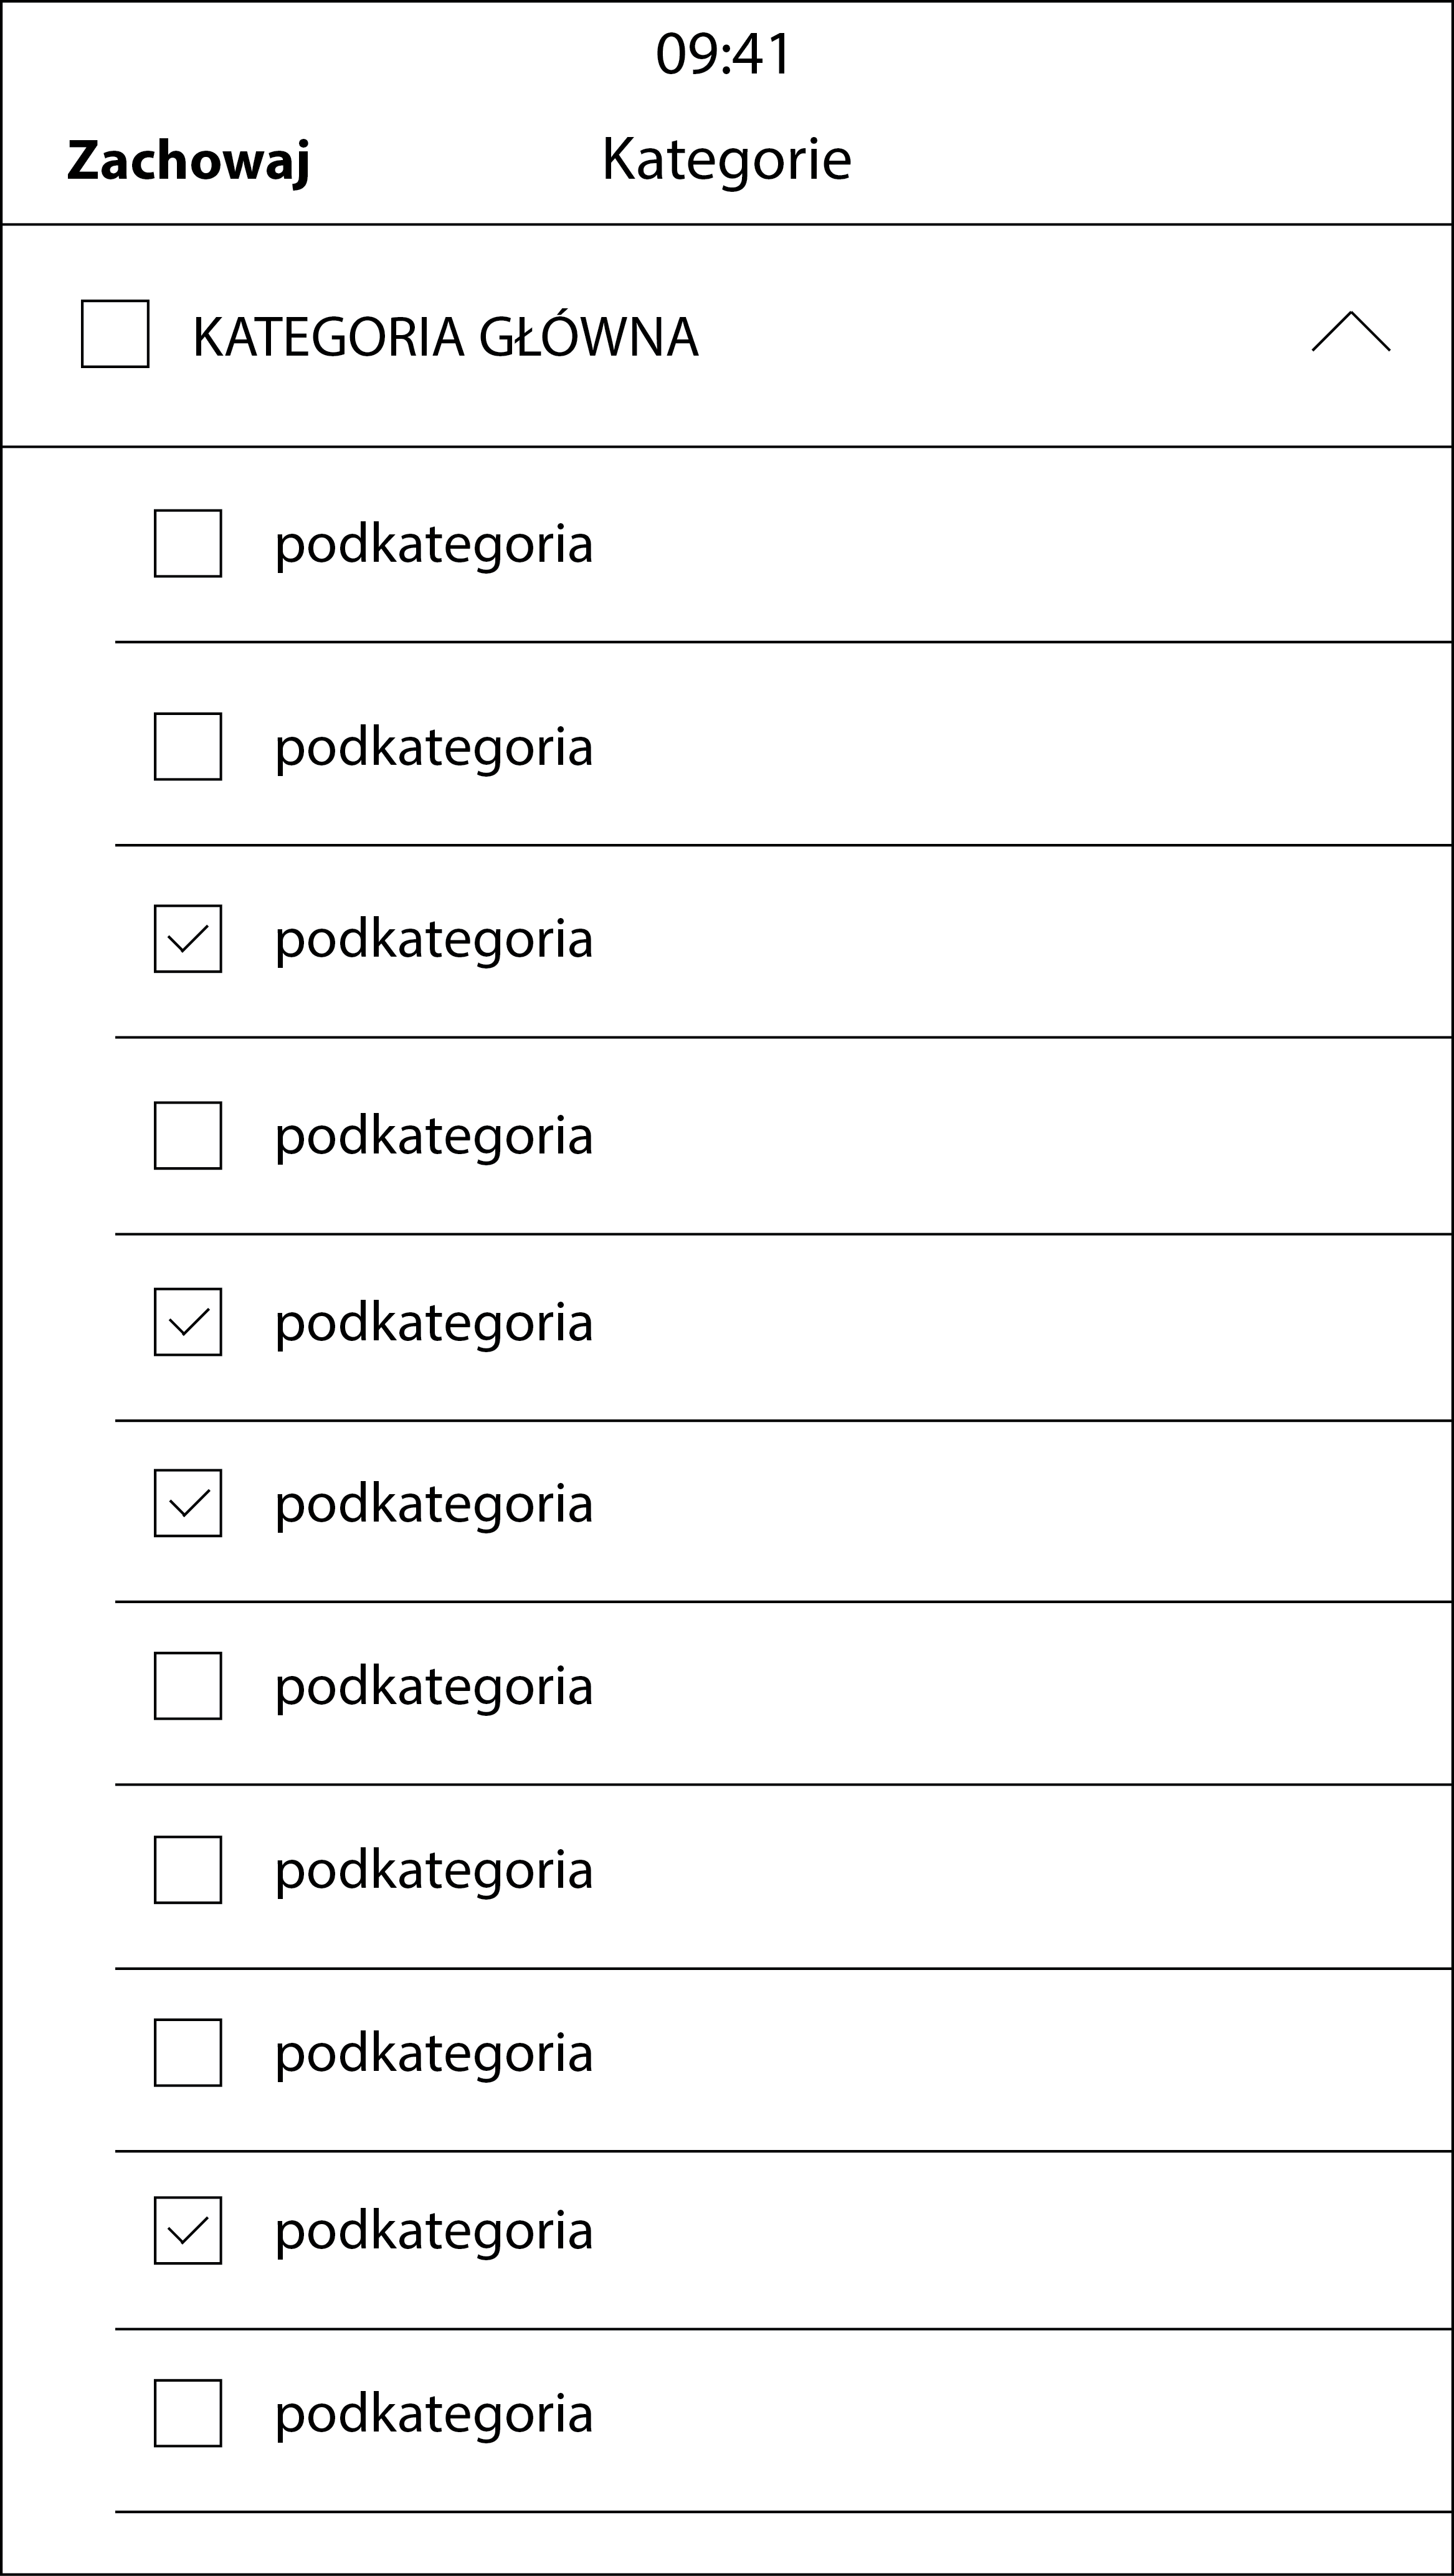
\includegraphics[width=0.4\linewidth]{img/CategoriesProject.png}
  \caption{Projekt ekranu wyboru kategorii}
  \label{fig:iosCategories}
\end{figure}

Kolejnym widokiem jest obiekt klasy \verb`CategoriesViewController`. Jest to widok posiadający komponent \verb`UITableView`, jednak w bardziej skomplikowanej konfiguracji niż widok \verb`SearchViewController`. W tabeli został zarejestrowany model komórki kategorii \verb`CategoryTableViewCell` oraz model nagłówka głównej kategorii \verb`MainCategoryHeaderView`. Tabela została stworzona jako tabela rozwijalna, tzn. po wyborze sekcji, wyświetlane są komórki do niej należące. Z powodu braku natywnego rozwiązania na tę funkcjonalność, została ona stworzona samodzielnie.

Widok posiada zmienną \verb`expandedHeaders`, która z początku jest wypełniona wartościami typu \verb`false`.
\begin{verbatim}
var expandedHeaders: [Bool] = []
...
func collapseAllHeaders() {
    let mainCategoriesCount =
        SessionManager.shared.mainCategories.count
    expandedHeaders =
        Array(repeating: false, count: mainCategoriesCount)
}
\end{verbatim}
Indeks każdego elementu tabeli odzwierciedla sekcję nagłówka. Pozwala to stwierdzić, które z sekcji są rozwinięte, a które zwinięte. Kliknięcie w przycisk rozwijania sekcji, uruchamia metodę ze specjalnie stworzonego na te potrzeby protokołu obsługującego nagłówek.
\begin{verbatim}
extension CategoriesViewController: MainCategoryHeaderViewDelegate {
    ...
    func expandSubcategories(
        usingHeader header: MainCategoryHeaderView)
    {
        var headerIsExpanded = expandedHeaders[header.section]
        headerIsExpanded = !headerIsExpanded
        header.isExpanded = headerIsExpanded
        expandedHeaders[header.section] = headerIsExpanded
        tableView.reloadData()
    }
}
\end{verbatim}
Powoduje ona przestawienie odpowiedniej wartości w tablicy \verb`expandedHeaders` na przeciwną, przekazanie jej do widoku i odświeżenie tabeli. Natywne metody delegatowe klasy \verb`UITableView` zostały uzupełnione w sposób obsługujący informacje dotyczące rozwiniętej/zwiniętej sekcji. Implementacja metody odpowiadającej za ilość wierszy, pochodząca z protokołu \verb`UITableViewDataSource` została zaprezentowana poniżej.
\begin{verbatim}
func tableView(_ tableView: UITableView,
    numberOfRowsInSection section: Int) -> Int
{
    if expandedHeaders[section] {
        return SessionManager.shared.mainCategories[section]
            .subcategories.count
    } else {
        return 0
    }
}
\end{verbatim}
W przypadku rozwiniętej sekcji zwraca ilość wierszy równą ilości podkategorii należących do kategorii głównej z danej sekcji. Dla zwiniętego nagłówka nie wyświetla żadnego wiersza.

Opisywany widok obsługuje także możliwość wyboru wierszy bądź nagłówków, w celu późniejszego wykorzystania wybranych kategorii. W tym celu również zostały wykorzystane zmienne służące do pamiętania stanu wyboru.
\begin{verbatim}
var selectedHeaders: [Bool] = []
var selectedCells: [IndexPath:Bool] = [:]
\end{verbatim}
Przedstawiają one zaznaczone nagłówki (obiekt typu \verb`Array`) oraz zaznaczone komórki (obiekt typu \verb`Dictionary`). Każde wybranie nagłówka, zmienia jego stan, jednocześnie wpływając na stan komórek należących do danej sekcji. Wybór nagłówka powoduje skorzystanie z metody przypisującej w słowniku \verb`selectedCells` zmienne typu \verb`Bool` do obiektów typu \verb`IndexPath`, które określają pozycję komórki w tabeli. Jednocześnie przypisując obiekty, komórki w zadanych pozycjach są zaznaczane lub odznaczane.

Nie tylko nagłówek może wpłynąć na stan komórki. Istnieje również odwrotna zależność. Wybór komórek także może wpłynąć na stan nagłówka (na przykład w~przypadku zaznaczenia wszystkich podkategorii). Obsługa tego zdarzenia została opisana poniższą metodą.
\begin{verbatim}
private func trySelectHeader(inSection section: Int) {
    let subcategories = SessionManager.shared
        .mainCategories[section].subcategories
    if subcategories.isEmpty { return }
    for (index, _) in subcategories.enumerated() {
        let indexPath = IndexPath(row: index, section: section)
        guard let selected = selectedCells[indexPath]
        else { return }
        if !selected {
            toggleHeader(inSection: indexPath.section,
                select: false)
            return
        }
    }
    toggleHeader(inSection: section, select: true)
}
\end{verbatim}

Dodatkowo obiekt typu \verb`CategoriesViewController` obsługuje zapis wybranych kategorii jak i załadowanie zaznaczonych już wcześniej kategorii, zaraz po wejściu na widok. 


\subsubsection{BookListViewController}

\begin{figure}[h]
  \centering
  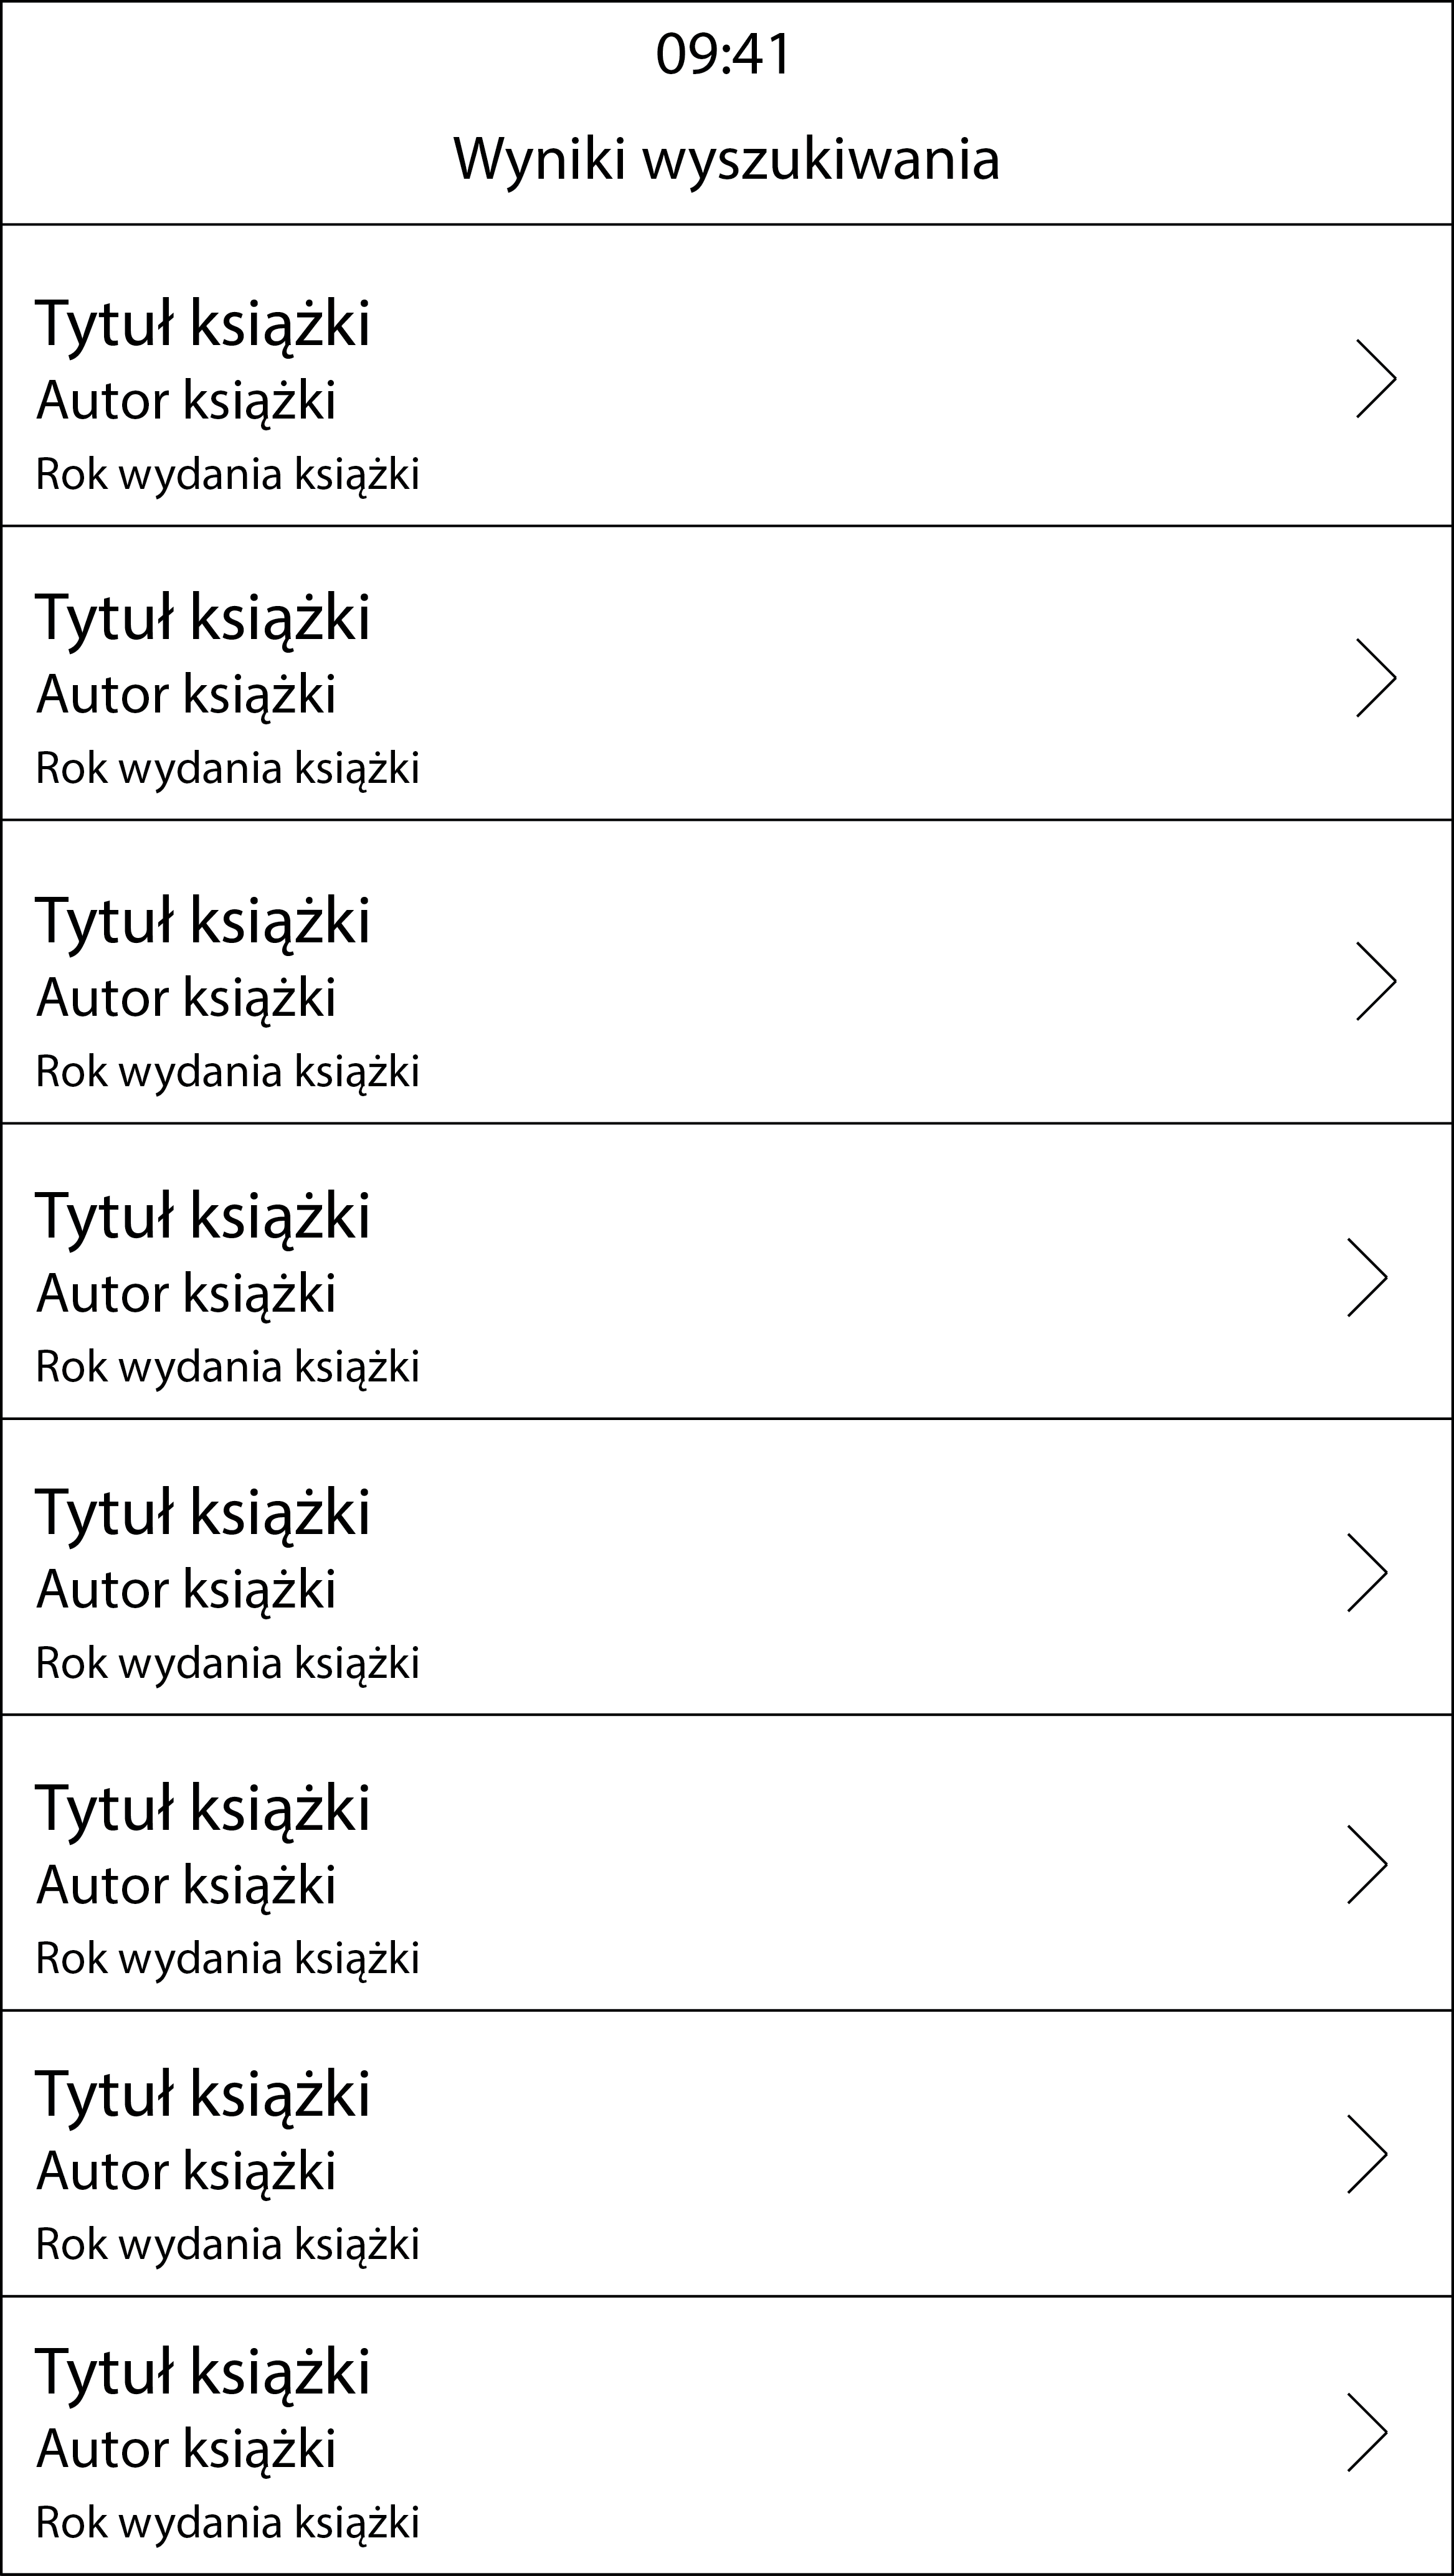
\includegraphics[width=0.4\linewidth]{img/BookListProject.png}
  \caption{Projekt ekranu listy książek}
  \label{fig:iosCategories}
\end{figure}

Obiekt klasy \verb`BookListViewController` jest następnym z widoków posiadających tabelę \verb`UITableView`. Służy do wyświetlania wyników wyszukiwania. Została w~nim zarejestrowana komórka typu \verb`BookTableViewCell`, która wyświetla tytuł oraz autora znalezionej książki. Tabela została przystosowana w taki sposób, aby wyświetlać pewną ilość książek, a w przypadku zaistniałej potrzeby, dociągać kolejną ich ilość. Metoda \verb`tryFetchMoreBooks(loadedIndexPath: IndexPath)`, która została zaimplementowana, jest wywoływana przy każdym ładowaniu się komórki na widoku. W przypadku, gdy ładowana jest szósta od końca komórka, metoda ta odpytuje usługę o kolejne książki. Gdy je otrzyma, dopisuje je do tablicy książek co powoduje odświeżenie widoku, ze zwiększoną liczbą znalezionych pozycji.

\begin{verbatim}
fileprivate func tryFetchMoreBooks(loadedIndexPath: IndexPath) {
    let rowWhenFetchNeeded = books.count - 5
    if loadedIndexPath.row == rowWhenFetchNeeded && canFetchMore {
        offset += DefaultValues.BOOKS_PER_FETCH
        RequestManager.shared.getBooks(
            withOffset: offset,
            completion: appendFetchedBooks)
    }
}
fileprivate func appendFetchedBooks(_ fetchedBooks: [Book]) {
    if fetchedBooks.isEmpty {
        canFetchMore = false
        return
    }
    self.books.append(contentsOf: fetchedBooks)
}
\end{verbatim}

Widok przedstawiający listę książek, obsługuje dodatkowo natywne rozwiązanie typu \textit{3D Touch}. Pozwala ono na podgląd zawartości komórki oraz wykonanie dodatkowych akcji przed jej wyborem. W tym celu, zostało stworzone rozszerzenie klasy \verb`BookListViewController` obsługujące akcje mocnego przyciśnięcia wiersza (\textit{Peek}) oraz jego jeszcze mocniejszego dociśnięcia (\textit{Pop}).

\begin{verbatim}
extension BookListViewController: UIViewControllerPreviewingDelegate {
    //PEEK
    func previewingContext(
        _ previewingContext: UIViewControllerPreviewing,
        viewControllerForLocation location: CGPoint) -> UIViewController?
    {
        guard let indexPath = tableView.indexPathForRow(at: location),
            let cell = tableView.cellForRow(at: indexPath)
        else {
            return nil
        }
        let book = books[indexPath.row]
        let detailsVC = getBookDetailsViewController(forBook: book)
        previewingContext.sourceRect = cell.frame
        return detailsVC
    }
    //POP
    func previewingContext(
    _ previewingContext: UIViewControllerPreviewing,
    commit viewControllerToCommit: UIViewController) {
        let navigationController = UINavigationController(
            rootViewController: viewControllerToCommit)
        self.showDetailViewController(navigationController,
            sender: self)
    }
}
\end{verbatim}
Akcja \textit{3D Touch} jest obsługiwana jedynie na telefonach typu iPhone 6s i nowszych. Z~tego powodu należy po załadowaniu widoku upewnić się, czy jest sens rejestrowania metod szybkiego podglądu.
\begin{verbatim}
override func viewDidAppear(_ animated: Bool) {
    super.viewDidAppear(animated)
    if traitCollection.forceTouchCapability == .available {
        registerForPreviewing(with: self, sourceView: tableView)
    }
}
\end{verbatim}

Widok typu \verb`BookListViewController` posiada dodatkowo obsługę w przypadku, gdy ilość otrzymanych książek z usługi jest równa 0. Do obsługi pustego ekranu wykorzystana została biblioteka \textit{UIEmptyState} \cite{UIEmptyState}. Jest to mało rozpowszechniona biblioteka służąca do analizowania wyświetlanych informacji w tabeli \verb`UITableView` lub kolekcji \verb`UICollectionView`, która w przypadku liczby elementów do wyświetlenia równej 0, pokaże użytkownikowi dowolnie spersonalizowaną informację o braku danych do zaprezentowania.

Biblioteka ta jest napisana w stosunkowo przyjazny sposób dla programisty. W celu zastosowania jej funkcjonalności, należy zaimplementować dwa typy protokołów: \verb`UIEmptyStateDelegate` oraz \verb`UIEmptyStateDataSource`. Następnie można przejść do przypisywania potrzebnych zmiennych, które zostaną automatycznie wyświetlone w przypadku braku elementów do wyświetlenia na widoku.
\begin{verbatim}
extension BookListViewController:
    UIEmptyStateDelegate, UIEmptyStateDataSource
{
    fileprivate func setEmptyStateDelegates() {
        self.emptyStateDelegate = self
        self.emptyStateDataSource = self
    }
    var emptyStateBackgroundColor: UIColor {
        return .main
    }
    var emptyStateTitle: NSAttributedString {
        let title = R.string.localizable.noResults()
        let range = (title as NSString).range(of: title)
        let titleAttributedString =
            NSMutableAttributedString(string: title)
        let titleColor = UIColor.tintDark
        titleAttributedString.addAttribute(
            NSAttributedStringKey.foregroundColor,
            value: titleColor, range: range)
        return titleAttributedString
    }
    var emptyStateImage: UIImage? {
        let image = R.image.bookShelf()
            .maskWithColor(color: .tintDark)
        return image
    }
}
\end{verbatim}


\subsubsection{BookDetailsViewController}

\begin{figure}[h]
  \centering
  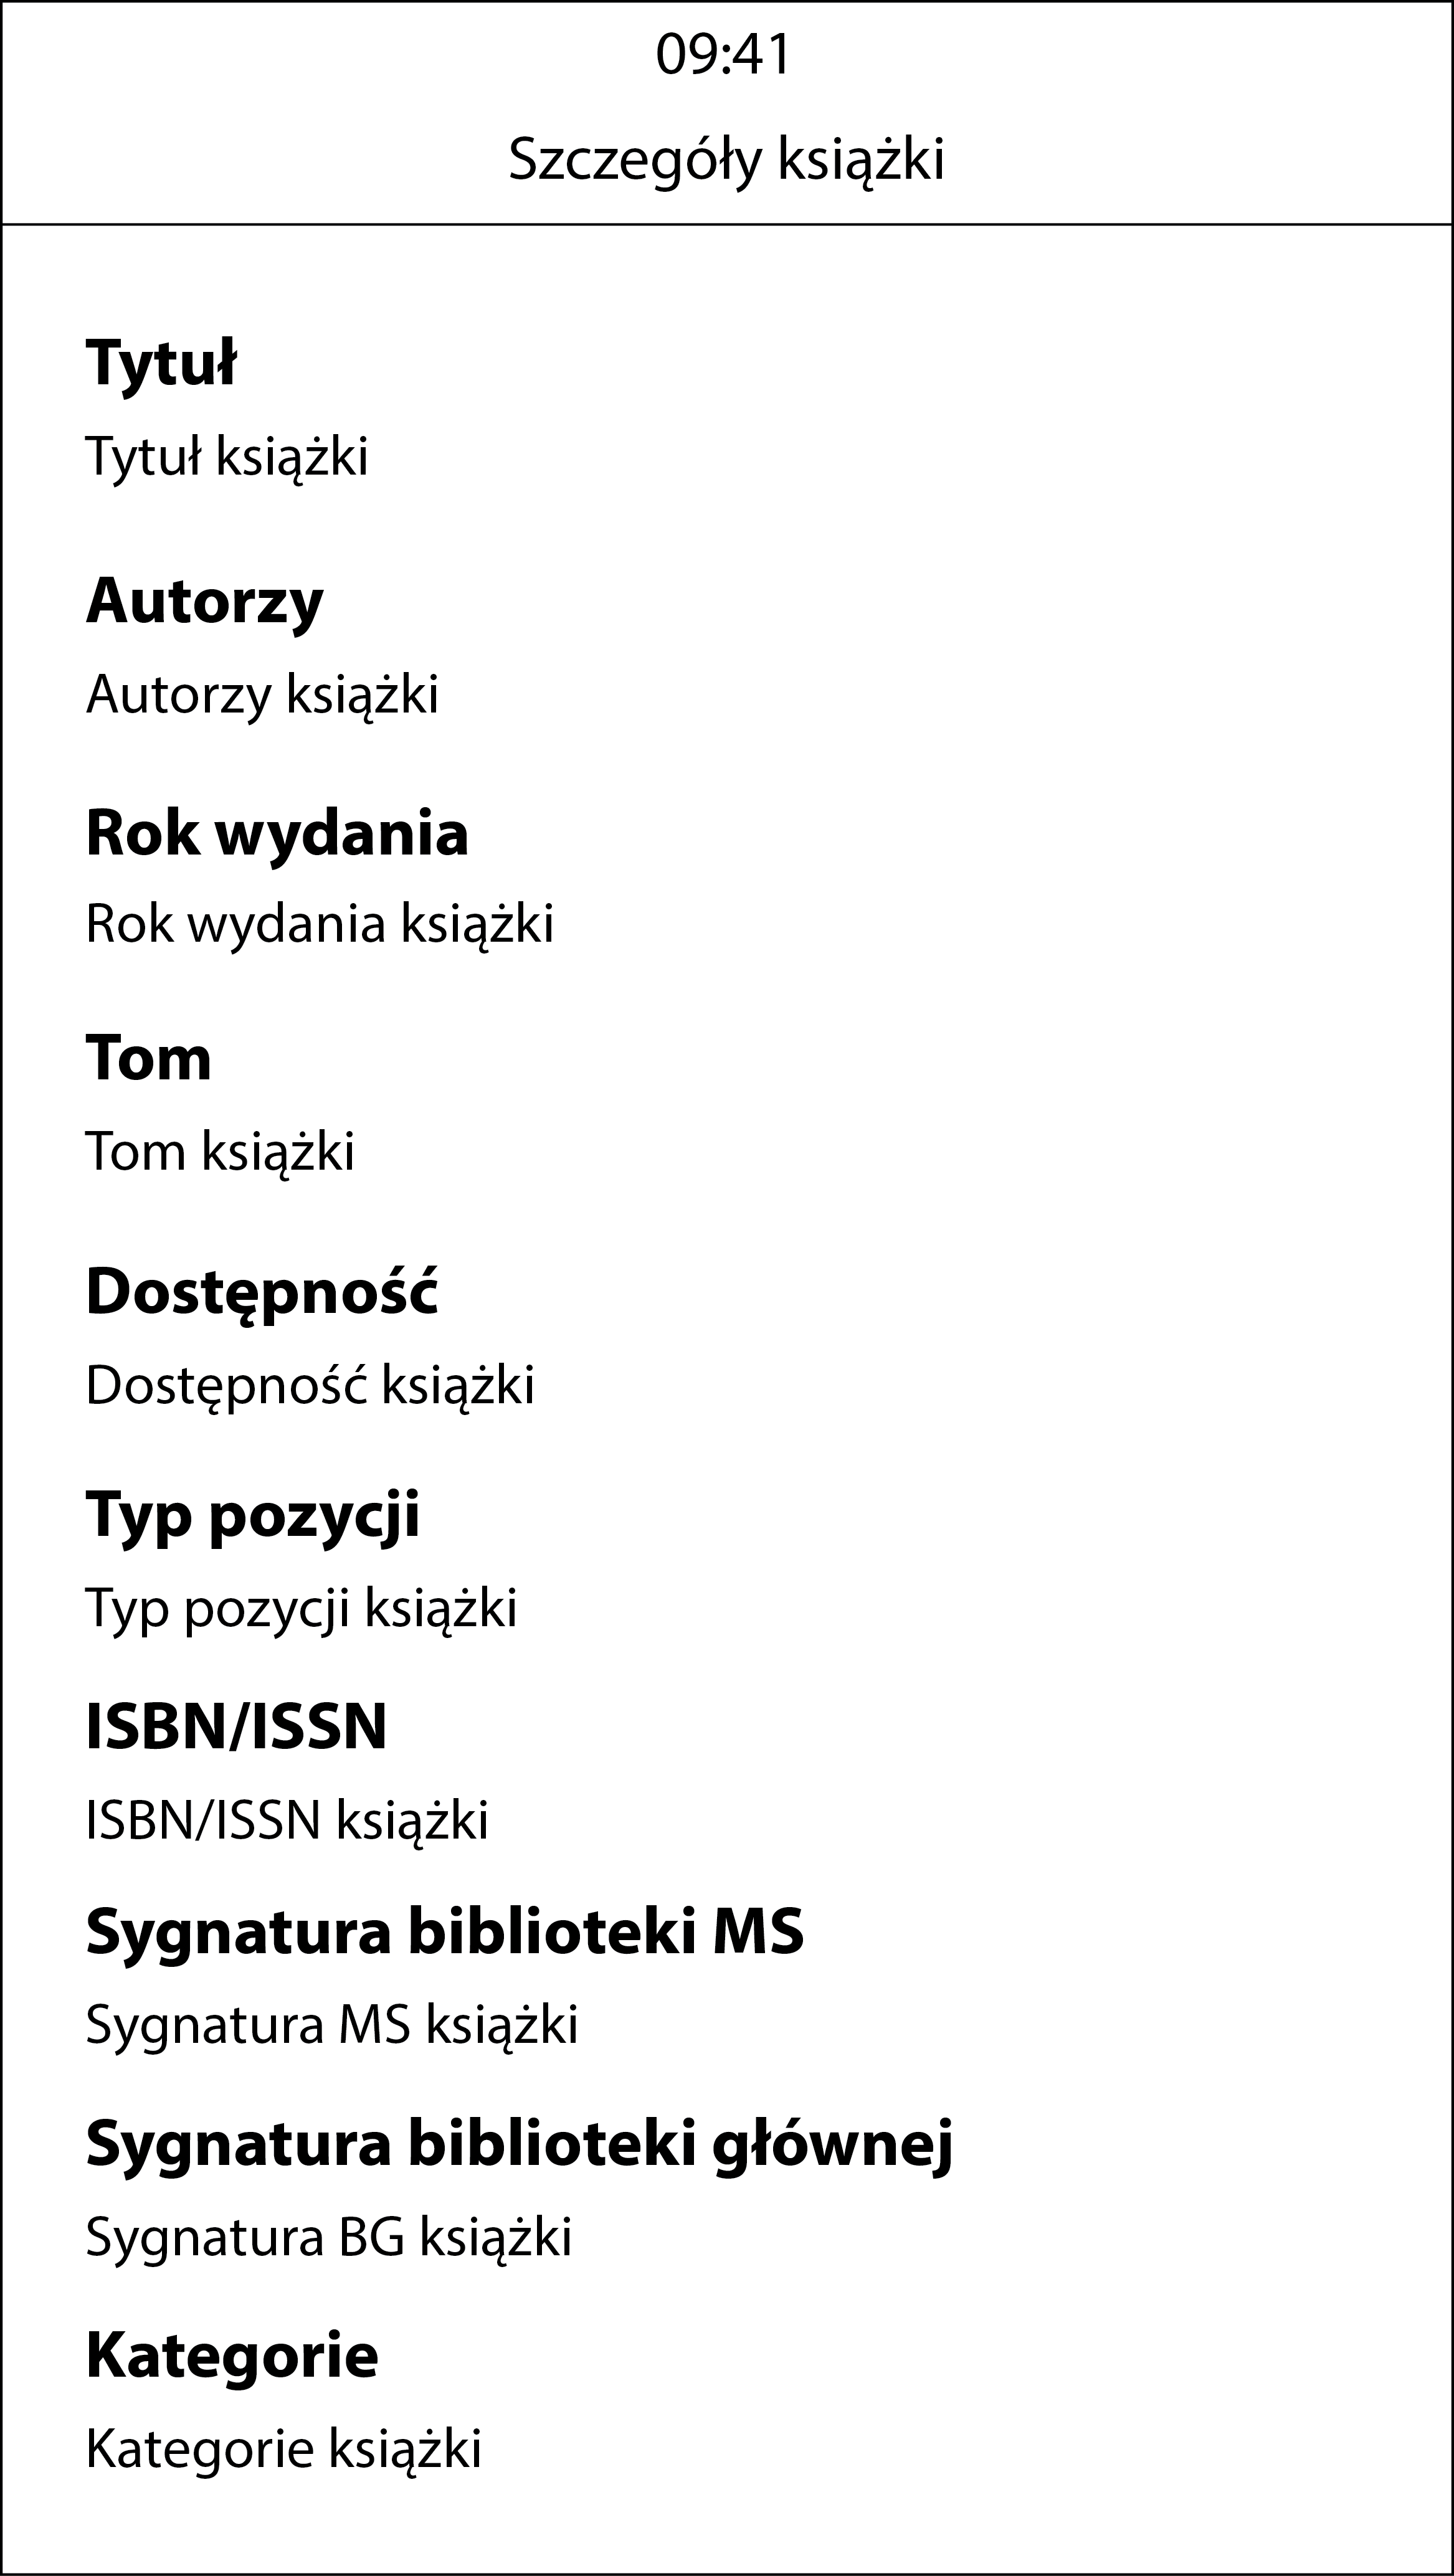
\includegraphics[width=0.4\linewidth]{img/DetailsProject.png}
  \caption{Projekt ekranu szczegółów książki}
  \label{fig:iosCategories}
\end{figure}

Klasa \verb`BookDetailsViewController` przedstawia obiekt widoku informacji o książce. Składa się ona tak jak inne widoki z tabeli \verb`UITableView`, a do wyświetlenia zawartości wykorzystuje komórkę typu \verb`BookDetailTableViewCell` posiadająca jedynie tytuł oraz zawartość pola opisującego książkę. Opisywana klasa widoku, jest dużo prostsza od poprzednich. Elementem wyróżniającym ją spośród pozostałych, jest zmienna typu \verb`[UIPreviewActionItem]`, która odpowiada za szybkie akcje w~trybie \textit{Peek}, będąc na poprzednim widoku typu \verb`BookListViewController`.
\begin{verbatim}
override var previewActionItems: [UIPreviewActionItem] {
    let copyTitleAction = UIPreviewAction(
        title: R.string.localizable.copyTitle(),
        style: .default) {
            (action, vc) in
            UIPasteboard.general.string = self.book?.bookTitle
    }
    let copyAuthorAction = UIPreviewAction(
        title: R.string.localizable.copyAuthor(),
        style: .default) {
            (action, viewcontroller) in
            UIPasteboard.general.string = self.book?.bookAuthors
    }
    return [copyTitleAction, copyAuthorAction]
}
\end{verbatim} 


\subsubsection{SessionManager}

\verb`SessionManager` to klasa odpowiadająca za zarządzanie, przechowywanie i udostępnianie danych do widoków podczas jednej sesji działania aplikacji. Klasa ta posiada trzy pola. Wystarczają one do zarządzania całą sesją, która jest aktywna, dopóki aplikacja znajduje się w pamięci RAM urządzenia.
\begin{itemize}
\item \verb`var searchedBook: Book!` -- pole odpowiadające za przetrzymywanie szablonowej, poszukiwanej przez użytkownika książki. Pole to jest aktualizowane z~każdą zmianą użytkownika na widoku wyszukiwania.
\item \verb`var mainCategories: [MainCategory]` -- wszystkie kategorie (główne wraz z podkategoriami) zaciągnięte z usługi po wejściu w aplikację.
\item \verb`var dictionaryTypes: DictionaryTypes!` -- wszystkie możliwe typy pozycji oraz stany dostępności książek. Otrzymywane są z usługi po otwarciu aplikacji.
\end{itemize}


Klasa \verb`SessionManager`, z powodu zarządzania całą sesją, została zaimplementowana z zastosowaniem wzorca projektowego Singleton. Zgodnie z jego założeniami, klasa posiada statyczną instancję oraz prywatny konstruktor.
\begin{verbatim}
class SessionManager {
    private init() {
        searchedBook = Book()
        dictionaryTypes = DictionaryTypes()
    }
    static let shared = SessionManager()
    ...
}
\end{verbatim}


\subsubsection{RequestManager}

Za odpytywanie usługi odpowiada klasa \verb`RequestManager`. Klasa ta jest również Singletonem. Jest ona napisana korzystając jedynie z natywnych rozwiązań języka \textit{Swift 4}. Dzięki implementacji odpowiednich protokołów przez klasy modelowe, metoda ta jest w stanie bezpośrednio stworzyć obiekt z danych, które przyszły z usługi w formacie \textit{.json}. Poniżej został przedstawiony przykład zaciągania z usługi obiektu tablicy wszystkich kategorii głównych.
\begin{verbatim}
func getCategories(completion: @escaping (([MainCategory])->())) {
    guard let request = getRequest(usingHttpMethod: "GET",
        forEndpoint: CATEGORY_ENDPOINT) else { return }
    URLSession.shared.dataTask(with: request) {
        (data, response, error) in
        if let error = error {
            NSLog(error.localizedDescription)
        }
        guard let data = data else { return }
        do {
            let mainCategories = try
                JSONDecoder().decode([MainCategory].self, from: data)
            completion(mainCategories)
        } catch let jsonError {
            NSLog(jsonError.localizedDescription)
            completion([])
        }
    }.resume()
}
\end{verbatim}

Każda z metod odpytujących usługę zaimplementowana jest korzystając z metody tworzącej typowy obiekt klasy \verb`URLRequest?`. Jest on tworzony na podstawie typu metody (w przypadku naszego projektu korzystamy jedynie z typów \textit{GET} oraz \textit{POST}) oraz końcówki adresu do którego powinno zostać wysłane zapytanie.
\begin{verbatim}
fileprivate func getRequest(
    usingHttpMethod httpMethod: String?,
    forEndpoint endpoint: String) -> URLRequest?
{
    let address = URL_STRING + endpoint
    guard let url = URL(string: address) else { return nil }
    var request = URLRequest(url: url)
    request.httpMethod = httpMethod
    request.setValue("application/json",
        forHTTPHeaderField: "Content-Type")
    return request
}
\end{verbatim}


\subsection{Interfejs użytkownika}


\subsubsection{Wyszukiwarka książek}

Aplikacja po uruchomieniu, przechodzi bezpośrednio do ekranu wyszukiwarki książek, jak zostało przedstawione na rysunku \ref{fig:iosSearchEmpty}. Aplikacja do poprawnego działania wymaga połączenia użytkownika z internetem. W przypadku braku połączenia internetowego, na ekranie pojawi się stosowna informacja zaraz po wejściu na widok. Przycisk w lewym górnym roku pozwala na odświeżenie zawartości. Użytkownik ma możliwość uzupełnienia dowolnych pól, w zależności od poszukiwanej przez niego pozycji. 

\begin{figure}
\centering
\begin{minipage}{.5\textwidth}
    \centering
    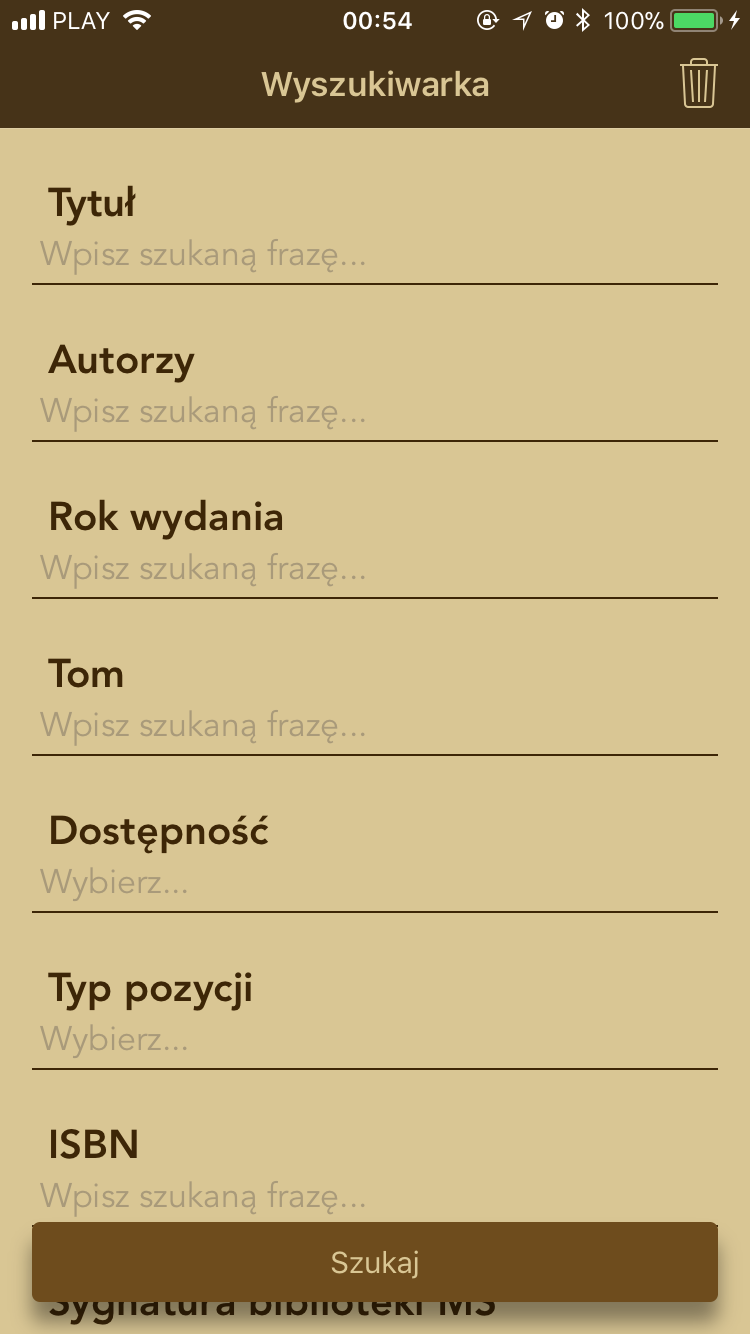
\includegraphics[width=0.8\linewidth]{img/iOS/ios1.png}
    \caption{Niewypełniony ekran wyszukiwania książki}
    \label{fig:iosSearchEmpty}
\end{minipage}%
\begin{minipage}{.5\textwidth}
    \centering
    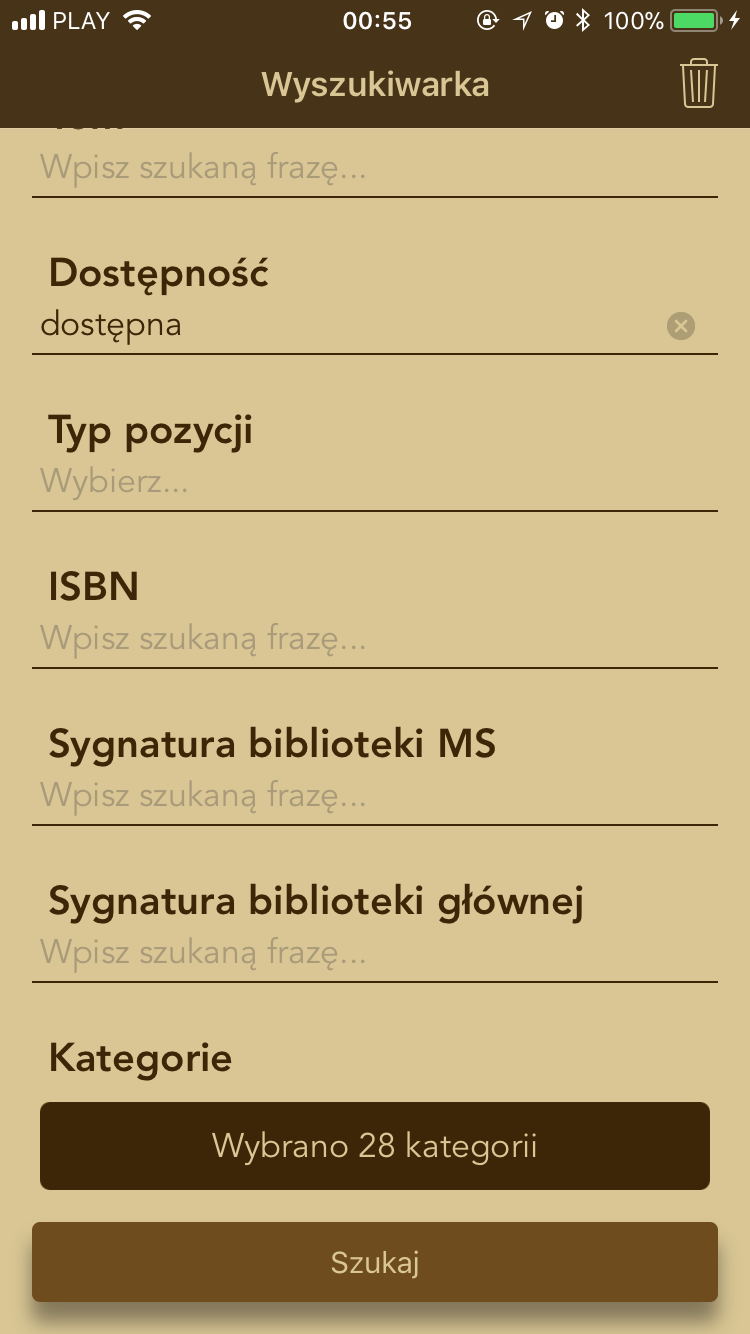
\includegraphics[width=0.8\linewidth]{img/iOS/ios3.png}
    \caption{Częściowo uzupełniony ekran wyszukiwania książki}
    \label{fig:iosSearchFilled}
\end{minipage}
\end{figure}

Pierwsze z pól są polami służącymi do uzupełnienia tekstu za pomocą klawiatury systemowej bądź wyboru jednego z kilku elementów z prostej listy. Ostatnia z komórek posiada przycisk przenoszący użytkownika do ekranu wyboru kategorii, jak na rysunku \ref{fig:iosCategories}. W prawym górnym rogu ekranu znajduje się przycisk, służący do wyczyszczenia wszystkich pól wyszukiwarki. Usunięcie dowolnego wypełnionego pola również jest możliwe -- wystarczy wybrać szary przycisk znajdujący się obok wypełnionego pola, jak na rysunku \ref{fig:iosSearchFilled}.

U dołu ekranu znajduje się przycisk wyszukiwania. Kliknięcie go, uruchamia wyszukiwanie, co jest oznajmione poprzez kręcące się kółeczko wewnątrz przycisku.


\subsubsection{Wybór kategorii}

Ekran kategorii, jest listą elementów posortowanych w sekcjach. Niektóre z sekcji są rozwijalne. Rozwinięcie sekcji pozwala użytkownikowi przejrzeć wszystkie podkategorie dla wybranej kategorii głównej. Użytkownik może na tym ekranie dokonać wyboru zakresu poszukiwanej przez niego książki. W przypadku wyboru kategorii głównej, zaznaczane są automatycznie wszystkie jej podkategorie. W prawym górnym rogu znajduje się przycisk z ikoną kosza. Pozwala on wyczyścić wybrane kategorie i zacząć wybór od nowa.


\begin{figure}[h]
  \centering
  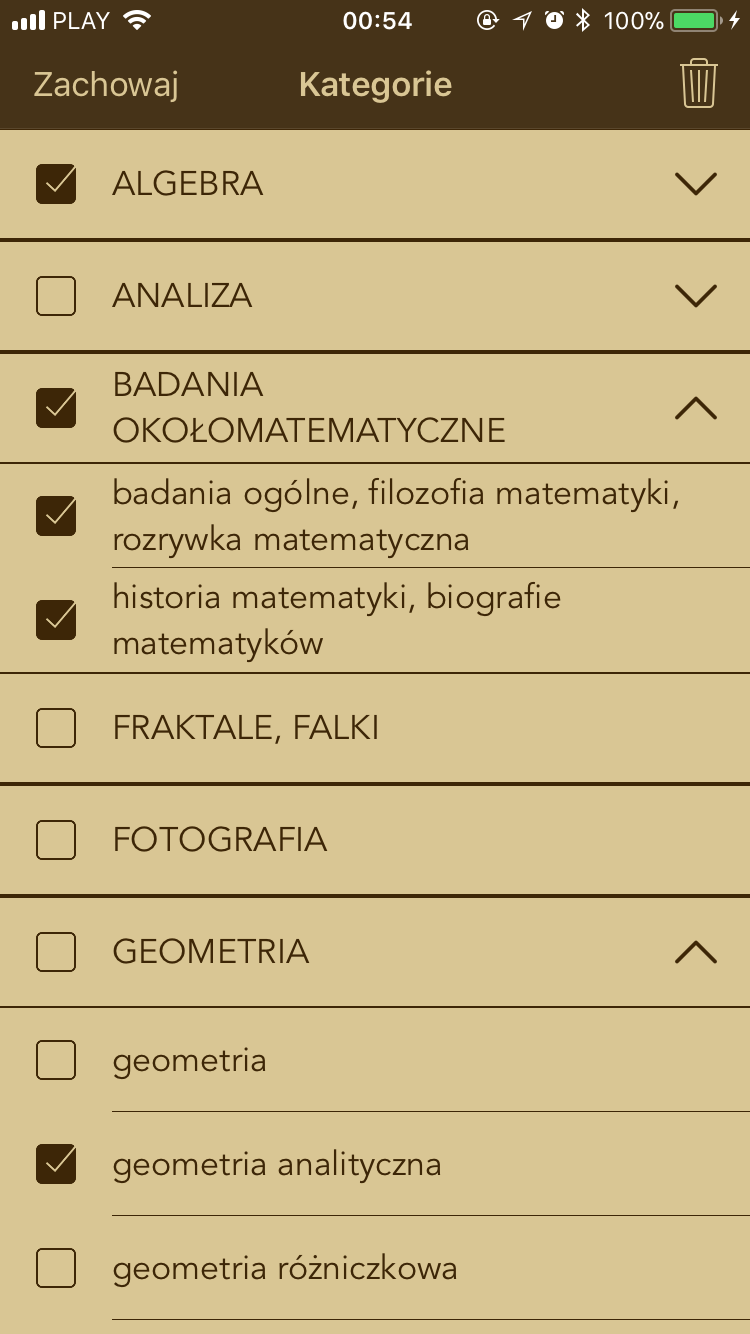
\includegraphics[width=0.4\linewidth]{img/iOS/ios2.png}
  \caption{Ekran wyboru kategorii}
  \label{fig:iosCategories}
\end{figure}

W lewym górnym rogu umiejscowiony jest przycisk zapisu wybranych kategorii. Jego wybór przenosi użytkownika z powrotem na ekran wyszukiwania. Po powrocie, przycisk do wyboru kategorii wyświetla ich konkretną ilość jaka została wybrana przez użytkownika. Zostało to przedstawione na rysunku \ref{fig:iosSearchFilled}.


\subsubsection{Wyniki wyszukiwania}

Na ekranie wyszukiwania, wybór przycisku odpowiadającego za szukanie, przekierowuje użytkownika do ekranu Wyników wyszukiwania. W przypadku nie znalezienia żadnej pozycji pasującej do zapytania, wyświetlany jest ekran znajdujący się na rysunku \ref{fig:iosResultsEmpty}. Ekran z rysunku numer \ref{fig:iosResults}, przedstawia listę z poprawnie znalezionymi pozycjami. Składa się on z wierszy przedstawiających tytuły oraz autorów wyszukanych pozycji. Ilość wyszukanych książek jest równa 20 lub mniejsza. W przypadku, gdy jest ona maksymalna, użytkownik może przejść do dołu listy w celu doładowania i wyświetlenia kolejnych rekordów na widoku.

\begin{figure}
\centering
\begin{minipage}{.5\textwidth}
    \centering
    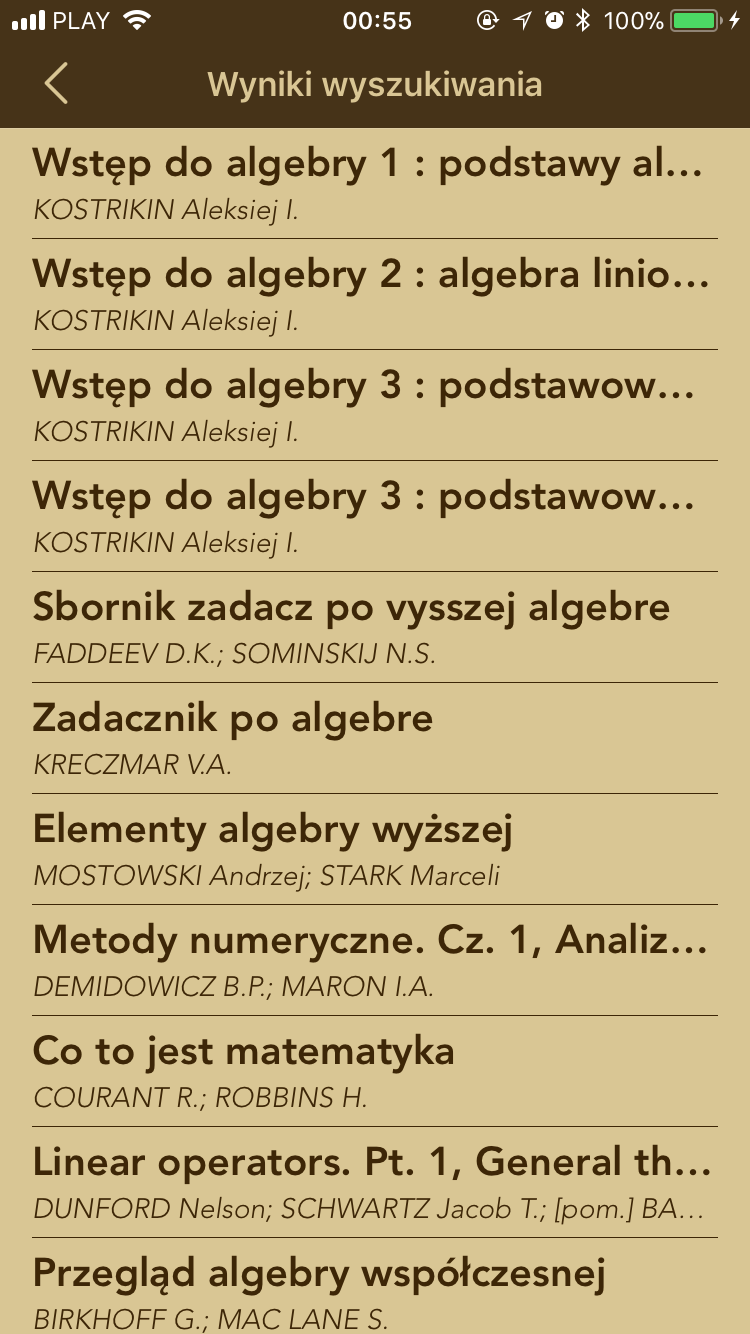
\includegraphics[width=0.8\linewidth]{img/iOS/ios4.png}
    \caption{Ekran wyników wyszukiwania}
    \label{fig:iosResults}
\end{minipage}%
\begin{minipage}{.5\textwidth}
    \centering
    
\includegraphics[width=0.8\linewidth]{img/iOS/ios5.png}
    \caption{Pusty ekran wyników}
    \label{fig:iosResultsEmpty}
\end{minipage}
\end{figure}

Użytkownik w celu przejścia dalej ma do wyboru dwie akcje:
\begin{enumerate}
\item Mocniejsze dociśnięcie ekranu w miejscu interesującej go pozycji.
\item Wybór interesującego go wiersza.
\end{enumerate}

\begin{figure}[h]
  \centering
  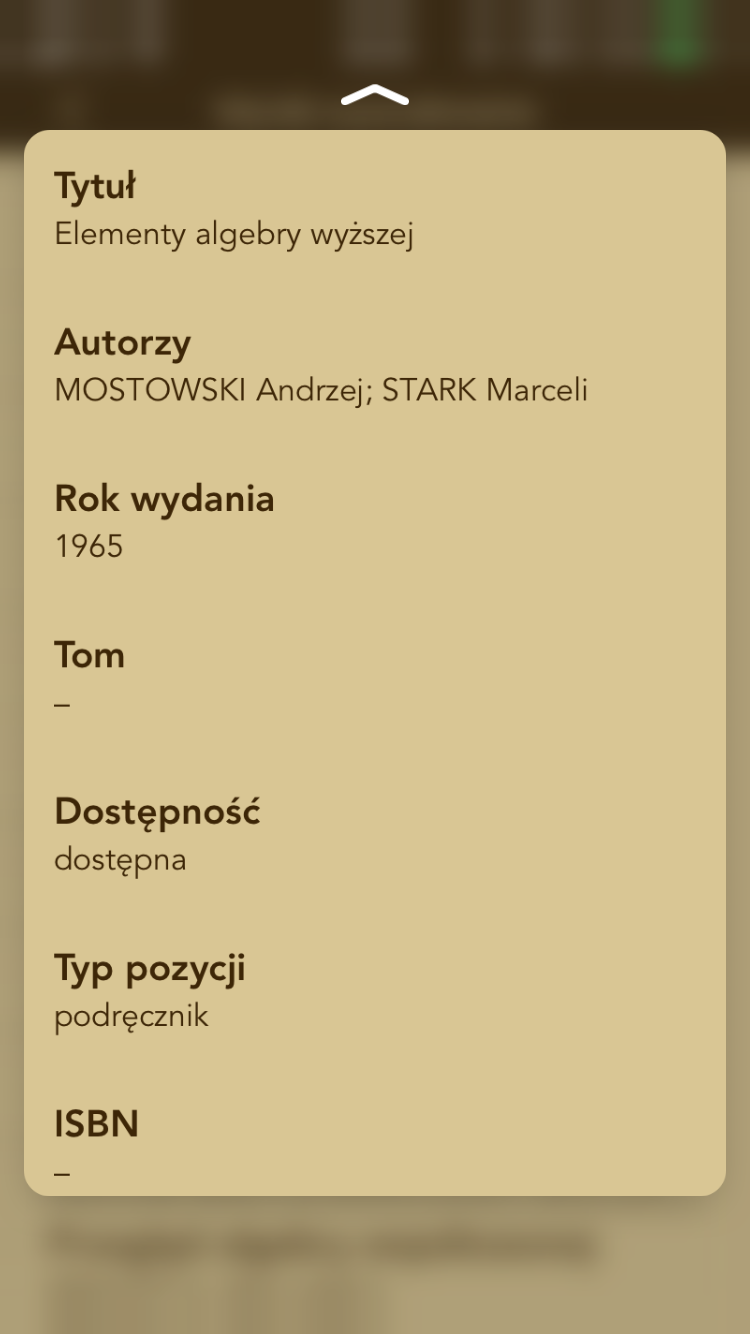
\includegraphics[width=0.4\linewidth]{img/iOS/ios6.png}
  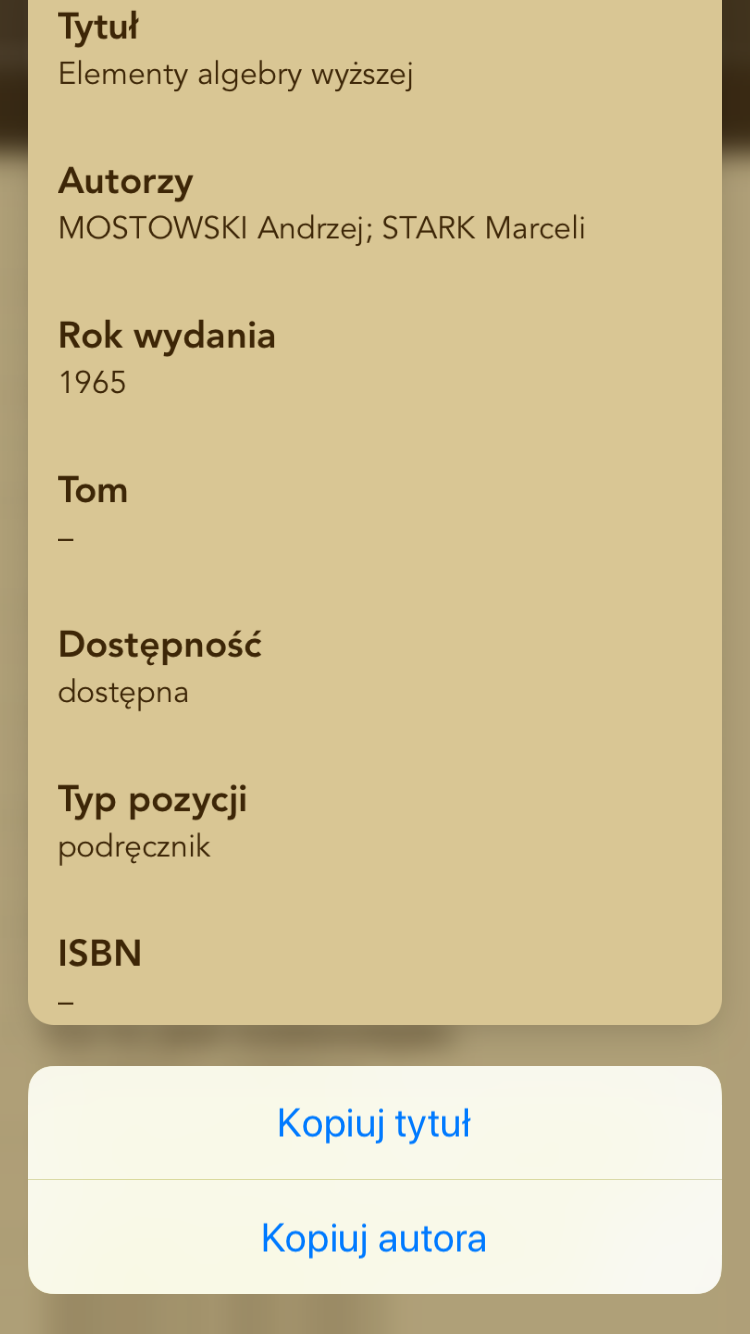
\includegraphics[width=0.4\linewidth]{img/iOS/ios7.png}
  \caption{Ekrany obsługujące akcje \textit{3D Touch}}
  \label{fig:3DTouch}
\end{figure}

Pierwsza opcja jest dostępna jedynie dla telefonów z opcją \textit{3D Touch} wbudowaną w ekran. W przypadku opcji 1., użytkownik otrzymuje na ekranie podgląd szczegółów książki, który przedstawiono na rysunku \ref{fig:3DTouch}. Przesunięcie go ku górze, spowoduje wyświetlenie się u dołu dodatkowych opcji. Będą to opcje umożliwiające skopiowanie tytułu bądź autora do schowka. Przeciągnięcie widoku podglądu w dół, spowoduje jego ukrycie. W przypadku jego jeszcze mocniejszego dociśnięcia, użytkownik zostanie przekierowany do ekranu. Analogiczna sytuacja ma miejsce podczas wyboru opcji numer 2., czyli zwykłego wyboru wiersza z książką.

W celu powrotu i rozpoczęcia szukania książki od początku, użytkownik może wybrać przycisk w lewym górnym rogu. Kliknięcie go, spowoduje powrót do ekranu wyszukiwania.

\subsubsection{Szczegóły książki}

Jest to ekran przedstawiony na rysunku \ref{fig:bookDetails}. Jest on prezentowany użytkownikowi od spodu, po wyborze jednej z komórek opisujących książkę. Przedstawia prostą przesuwaną listę elementów dotyczących wybranej książki. Przycisk w prawej górnej części ekranu pozwala schować widok i wrócić do poprzedniego ekranu wszystkich wyszukanych pozycji.

\begin{figure}[h]
  \centering
  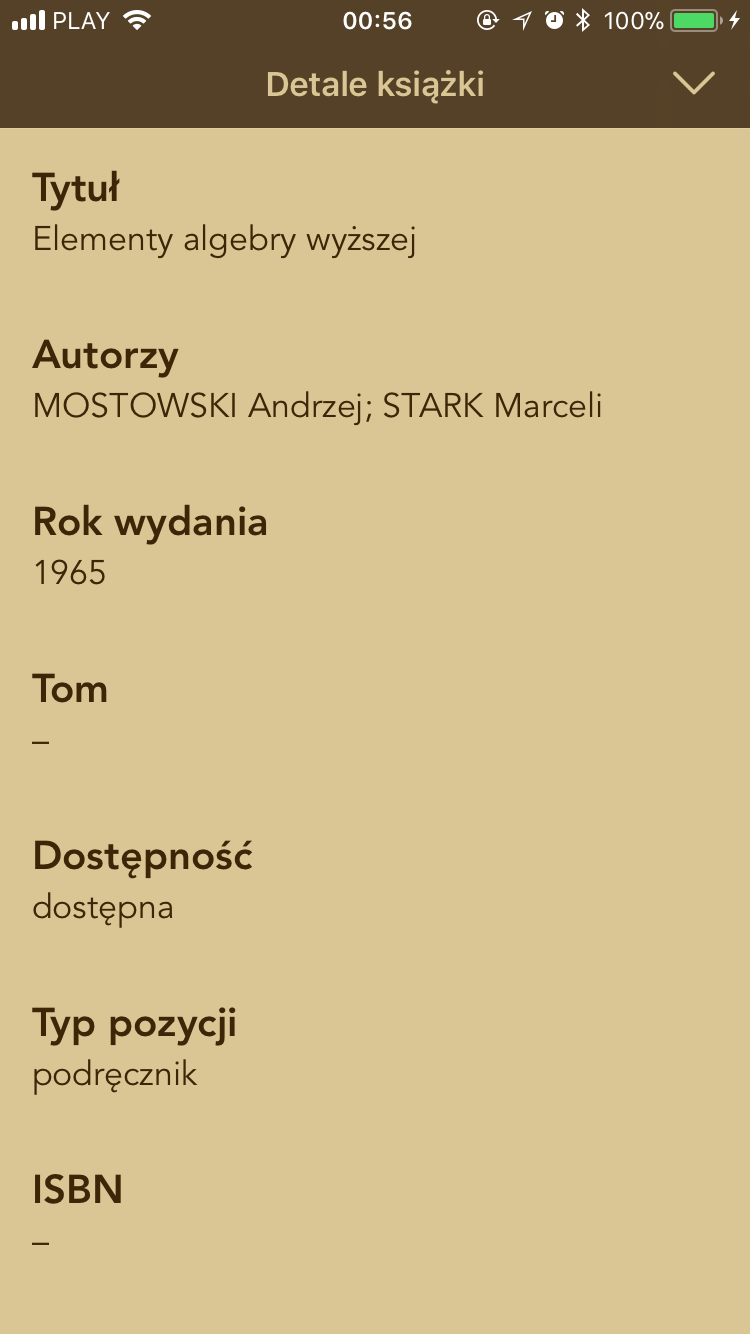
\includegraphics[width=0.4\linewidth]{img/iOS/ios8.png}
  \caption{Szczegóły książki}
  \label{fig:bookDetails}
\end{figure}


\section{Zakończenie}

Tworząc aplikację serwerową w tak małej grupie dla całego wydziału, mogliśmy znacznie poszerzyć swoją wiedzę jednocześnie rozwijając się w~zakresie pracy zespołowej. Dodatkowo w celu lepszego porozumienia się z wieloma osobami, z którymi pracowaliśmy i dyskutowaliśmy podczas wytwarzania tej aplikacji, musieliśmy poszerzyć swoje zdolności interpersonalne. Bez ich pomocy byłoby nam ciężko dopracować wiele spraw związanych z dostosowaniem obsługi, a także wyglądem aplikacji dla klienta.

Cały projekt aplikacji mobilnych jak i aplikacji webowej został omówiony i wielokrotnie prezentowany oraz testowany z Panią mgr inż. Martyną Maciaszczyk, która była osobą zatwierdzającą wszystkie postanowienia oraz zmiany w widoku wszystkich aplikacji. Proces ten przebiegał stosunkowo długo, jednak był bardzo pouczający.

Interfejs graficzny był jednym z problemów wytworzenia takiego systemu. Bardzo trudne jest dostosowanie do siebie wszystkich aplikacji pod względem wyglądu. Strona internetowa zawsze będzie nieco inna od aplikacji mobilnej, ponieważ istnieje wiele różnic dotyczących założeń działania, obsługi, czy też przyzwyczajeń i wymagań użytkownika od danego systemu. Z tego powodu aplikacja internetowa dla administratora różni się od aplikacji mobilnych przeznaczonych przede wszystkim dla studentów. Największym problemem było dostosowanie do siebie obu aplikacji mobilnych na systemy Android i iOS. Każdą z nich pisała inna osoba, więc założenia dotyczące projektu musiały być dokładnie ustalone, a każda późniejsza edycja ponosiła za sobą modyfikacje na obu platformach, co przekładało się na dwukrotnie zwiększony czas potrzebny do realizacji danej zmiany. Dodatkowo każda z platform ma inne natywne narzędzia używane do tworzenia aplikacji. Systemy różnią się od siebie również wyglądem, co przyzwyczaja użytkowników do swoich rozwiązań. Z tego powodu aplikacje na dwa różne systemy nigdy nie mogą być identyczne jeśli chcą być intuicyjne dla ich grupy docelowej odbiorców.

Aplikacja serwerowa dla biblioteki została napisana w sposób łatwy do rozszerzenia. Jej wygodne i proste w obsłudze możliwości dodawania nowych książek do bazy, mogą być wykorzystywane w przyszłości w celu powiększania ilości zbiorów dostępnych w bibliotece. Dodatkowo, warto byłoby dodać możliwość rezerwacji książki online, bezpośrednio z poziomu aplikacji mobilnej. Ciekawą opcją na dalszą przyszłość (z powodu dużego nakładu pracy), byłaby możliwość wypożyczania danej pozycji książki w postaci pliku o rozszerzeniu .pdf. Pozwoliłoby to nie tylko na zmniejszenie kolejek w bibliotece, ale także na możliwość dostępu do wszystkich książek z~urządzenia przenośnego bez potrzeby noszenia dużej ich ilości przy sobie. Co więcej, ilość książek w tym wypadku byłaby nieograniczona. Każdy ze studentów miałby swój wirtualny egzemplarz. Niestety byłoby to możliwe do osiągnięcia jedynie przy dużym nakładzie pracy z powodu dużej ilości skanów do wykonania a także stworzenia nowej usługi pozwalającej na ściąganie i zapisywanie plików na urządzeniu przenośnym.

Celem naszego projektu było utworzenie systemu dla Biblioteki Wydziału Matematyki Stosowanej na Politechnice Śląskiej w Gliwicach. Cel ten udało nam się osiągnąć zgodnie ze wszystkimi założeniami jakie zostały przed nami postawione. Mamy nadzieję, że w przyszłości uda się wdrożyć nasz system do użytku, i że posłuży on gronu odbiorców w taki sposób, w jaki byśmy chcieli, aby służył nam, gdy faktycznie go potrzebowaliśmy.


\begin{thebibliography}{12}

\bibitem{raportBN} http://www.bn.org.pl/aktualnosci/1338-czytelnictwo-polakow-2016-\%E2\%80\%93-raport-biblioteki-narodowej.html [dostęp: 10 lutego 2018]

\bibitem{DjangoAuth} https://docs.djangoproject.com/en/2.0/ref/contrib/auth/ [dostęp: 10 lutego 2018]
\bibitem{DjangoORM} https://docs.djangoproject.com/en/2.0/topics/db/queries/ [dostęp: 10 lutego 2018]
\bibitem{DjangoAdmin} https://docs.djangoproject.com/en/2.0/ref/contrib/admin/ [dostęp: 10 lutego 2018]
\bibitem{DjangoRest} http://www.django-rest-framework.org/  [dostęp: 10 lutego 2018]
\bibitem{DjangoTranslation} https://docs.djangoproject.com/en/2.0/topics/i18n/translation/ [dostęp: 10 lutego 2018]
\bibitem{DjangoModel} https://docs.djangoproject.com/en/2.0/topics/db/models/ [dostęp: 10 lutego 2018]
\bibitem{DjangoOfficial} https://docs.djangoproject.com/pl/2.0/intro/overview/ [dostęp: 10 lutego 2018]
\bibitem{djangobook} A. Mele, ,,Django. Praktyczne tworzenie aplikacji sieciowych'' Helion, 2015.
\bibitem{linuxAdmin} E. Nemeth, G. Snyder, T. Hein, B. Whaley, ,,Unix i Linux. Przewodnik
administratora systemów.'', Wydanie IV, Helion, 2011.


\bibitem{clean_code}
Robert C. Martin. 
\textit{Czysty kod. Podręcznik dobrego programisty}. 
Wydawnictwo Helion, 2010, ISBN 978-83-283-1401-6.
\bibitem{Swift1} The Swift Programming Language (Swift 4.0.3)
\bibitem{Swift2} Using Swift with Cocoa and Objective-C (Swift 4.0.3)
\bibitem{iosStatistics} https://developer.apple.com/support/app-store/ [dostęp: 10 lutego 2018]
\bibitem{AppleDeveloper} https://developer.apple.com/documentation/ [dostęp: 10 lutego 2018]
\bibitem{Rswift} https://github.com/mac-cain13/R.swift [dostęp: 10 lutego 2018]
\bibitem{JGProgressHUD} https://github.com/JonasGessner/JGProgressHUD
\bibitem{UIEmptyState} https://github.com/luispadron/UIEmptyState [dostęp: 10 lutego 2018]

\bibitem{javaOracle} J. Gosling, B. Joy, G. Steele, G. Bracha, A. Buckley. \textit{The Java® Language Specification. Java SE 8 Edition}. Oracle America, 2015.
\bibitem{androidStudioDev} https://developer.android.com/studio/releases/index.html [dostęp: 10 lutego 2018]
\bibitem{androidStatistics} https://developer.android.com/about/dashboards/index.html [dostęp: 10 lutego 2018]
\bibitem{crashlytics} https://fabric.io/kits/android/crashlytics [dostęp: 10 lutego 2018]
\bibitem{butterknife} http://jakewharton.github.io/butterknife/ [dostęp: 10 lutego 2018]
\bibitem{PPPAndroida} S. Madej, \textit{Przybornik Pragmatycznego Programisty
Androida}. Wydanie Pierwsze, 2015.
\bibitem{mvpBook} P. Mainkar, \textit{Expert Android Programming}. Packt Publishing, 2017, ISBN 9781786468956.
\bibitem{dagger2} https://github.com/codepath/android$\_$guides/wiki/Dependency-Injection-with-Dagger-2 [dostęp: 10 lutego 2018]
\bibitem{retrofit} http://square.github.io/retrofit/ [dostęp: 10 lutego 2018]
\bibitem{rxjava2} https://github.com/ReactiveX/RxJava [dostęp: 10 lutego 2018]
\bibitem{constraintLayout} https://developer.android.com/reference/android/support/constraint/ConstraintLayout.html [dostęp: 10 lutego 2018]
\bibitem{textInputEditText} https://developer.android.com/reference/android/support/design/widget/TextInputEditText.html [dostęp: 10 lutego 2018]

\end{thebibliography}
\end{document}
